\documentclass[../Head/report.tex]{subfiles}
\begin{document}
\section{Results}
\label{sec:results}

\subsection{Simulation}

\subsubsection{GPS to vision ArUco pose estimation}

\begin{figure}[H]
    \centering
    \begin{subfigure}[t]{.337\textwidth}
        \centering
        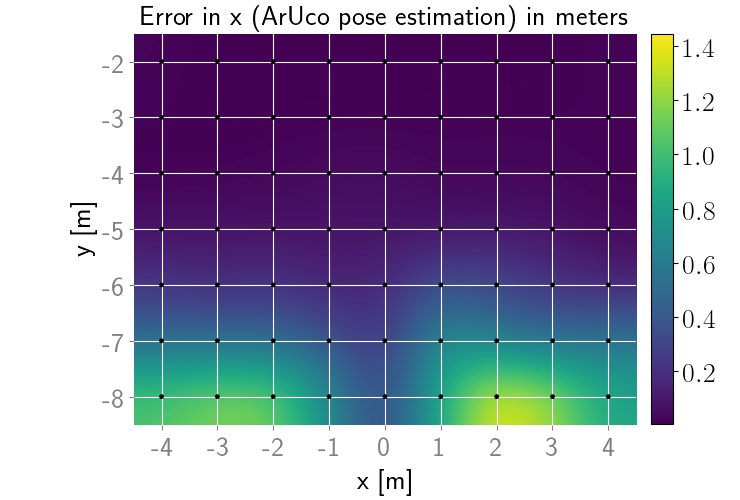
\includegraphics[width=\textwidth]{../Figures/GPS2Vision_pose_estimation_test/test1_aruco_board_width_0.2_space_0.1/aruco_pose_estimation_error_x.png}
        \caption{}
        \label{fig:GPS2Vision_pose_estimation_test1_error_x}
    \end{subfigure}
    \hspace{-0.9em}
    \begin{subfigure}[t]{.337\textwidth}
        \centering
        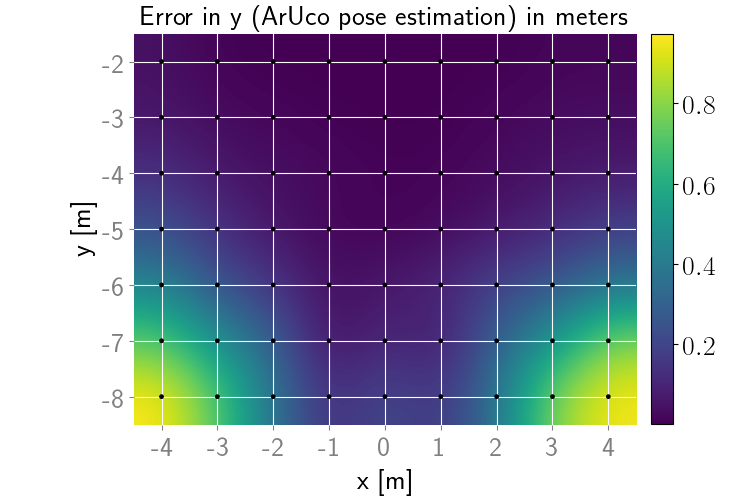
\includegraphics[width=\textwidth]{../Figures/GPS2Vision_pose_estimation_test/test1_aruco_board_width_0.2_space_0.1/aruco_pose_estimation_error_y.png}
        \caption{}
        \label{fig:GPS2Vision_pose_estimation_test1_error_y}
    \end{subfigure}
    \hspace{-0.9em}
    \begin{subfigure}[t]{.337\textwidth}
        \centering
        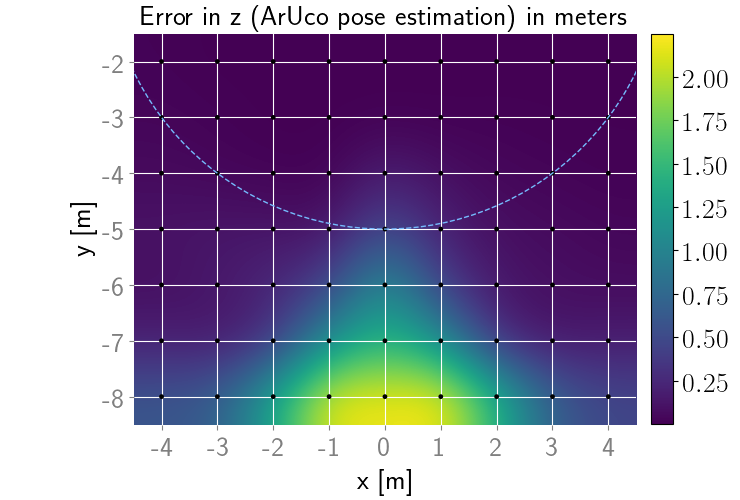
\includegraphics[width=\textwidth]{../Figures/GPS2Vision_pose_estimation_test/test1_aruco_board_width_0.2_space_0.1/aruco_pose_estimation_error_z.png}
        \caption{}
        \label{fig:GPS2Vision_pose_estimation_test1_error_z}
    \end{subfigure}
    \caption{}
    \label{fig:GPS2Vision_pose_estimation_test1_error_pos}
\end{figure}

\begin{figure}[H]
    \centering
    \begin{subfigure}[t]{.337\textwidth}
        \centering
        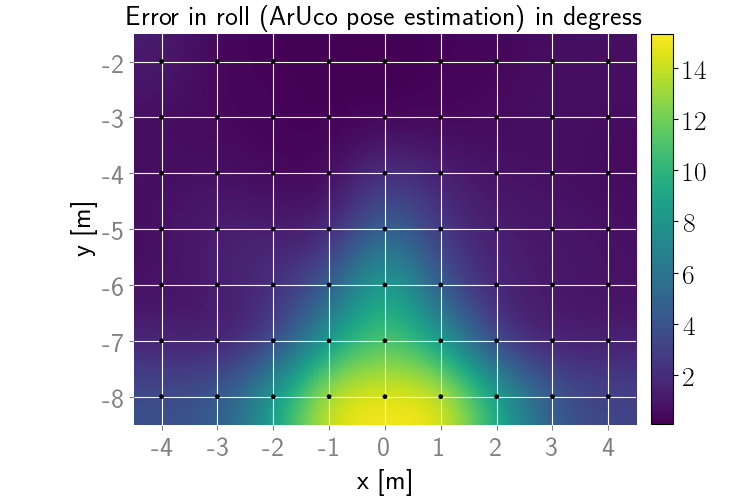
\includegraphics[width=\textwidth]{../Figures/GPS2Vision_pose_estimation_test/test1_aruco_board_width_0.2_space_0.1/aruco_pose_estimation_error_roll.png}
        \caption{}
        \label{fig:GPS2Vision_pose_estimation_test1_error_roll}
    \end{subfigure}
    \hspace{-0.9em}
    \begin{subfigure}[t]{.337\textwidth}
        \centering
        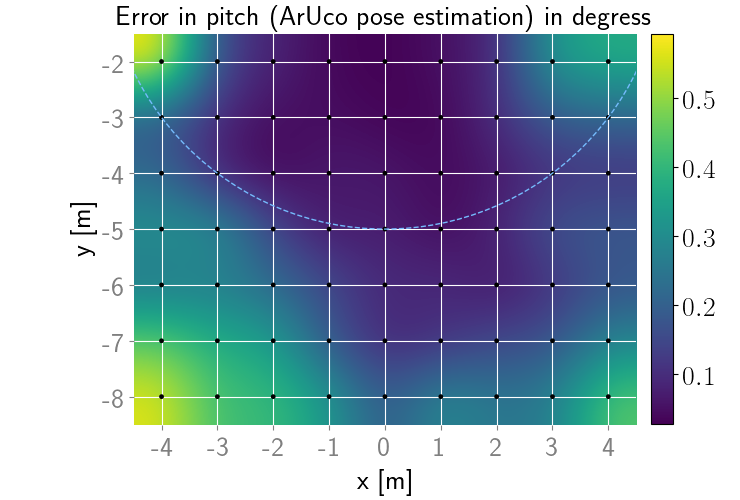
\includegraphics[width=\textwidth]{../Figures/GPS2Vision_pose_estimation_test/test1_aruco_board_width_0.2_space_0.1/aruco_pose_estimation_error_pitch.png}
        \caption{}
        \label{fig:GPS2Vision_pose_estimation_test1_error_pitch}
    \end{subfigure}
    \hspace{-0.9em}
    \begin{subfigure}[t]{.337\textwidth}
        \centering
        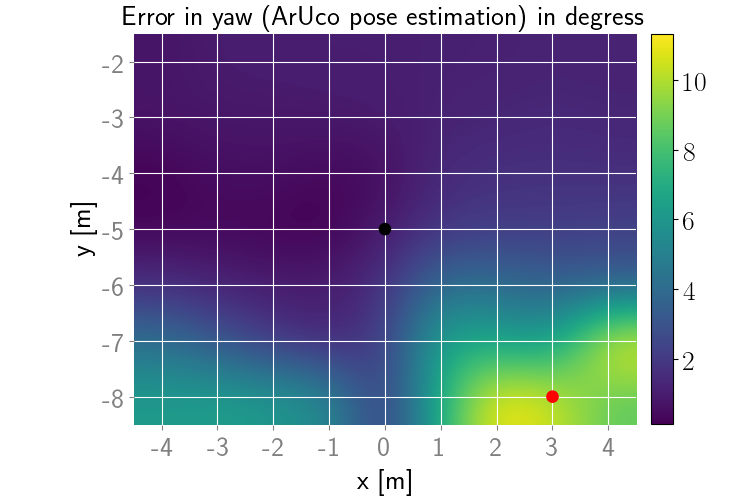
\includegraphics[width=\textwidth]{../Figures/GPS2Vision_pose_estimation_test/test1_aruco_board_width_0.2_space_0.1/aruco_pose_estimation_error_yaw.png}
        \caption{}
        \label{fig:GPS2Vision_pose_estimation_test1_error_yaw}
    \end{subfigure}
    \caption{}
    \label{fig:GPS2Vision_pose_estimation_test1_error_ori}
\end{figure}

\begin{figure}[H]
    \centering
    \begin{subfigure}[t]{.337\textwidth}
        \centering
        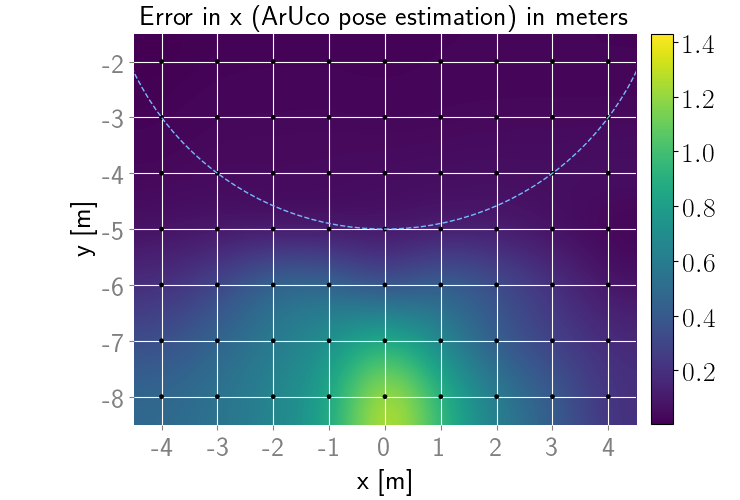
\includegraphics[width=\textwidth]{../Figures/GPS2Vision_pose_estimation_test/test2_aruco_board_width_0.3_space_0.15/aruco_pose_estimation_error_x.png}
        \caption{}
        \label{fig:GPS2Vision_pose_estimation_test2_error_x}
    \end{subfigure}
    \hspace{-0.9em}
    \begin{subfigure}[t]{.337\textwidth}
        \centering
        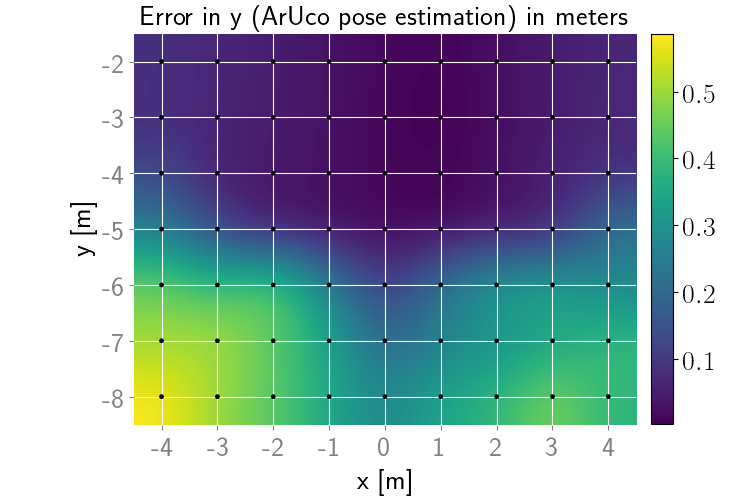
\includegraphics[width=\textwidth]{../Figures/GPS2Vision_pose_estimation_test/test2_aruco_board_width_0.3_space_0.15/aruco_pose_estimation_error_y.png}
        \caption{}
        \label{fig:GPS2Vision_pose_estimation_test2_error_y}
    \end{subfigure}
    \hspace{-0.9em}
    \begin{subfigure}[t]{.337\textwidth}
        \centering
        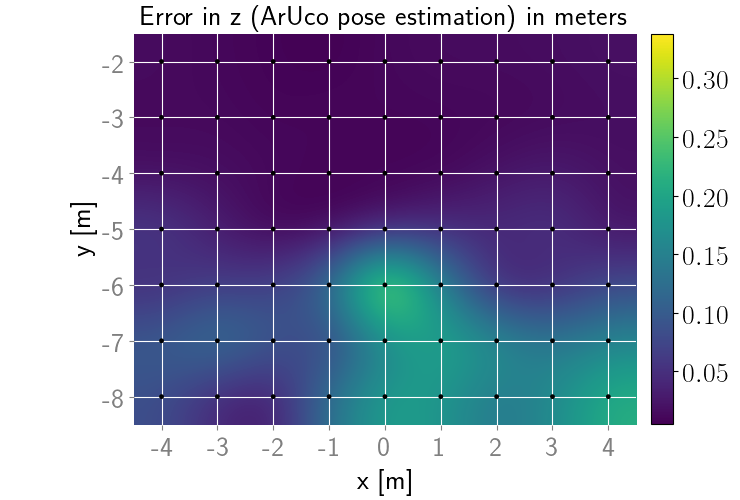
\includegraphics[width=\textwidth]{../Figures/GPS2Vision_pose_estimation_test/test2_aruco_board_width_0.3_space_0.15/aruco_pose_estimation_error_z.png}
        \caption{}
        \label{fig:GPS2Vision_pose_estimation_test1_error_z}
    \end{subfigure}
    \caption{}
    \label{fig:GPS2Vision_pose_estimation_test2_error_pos}
\end{figure}

\begin{figure}[H]
    \centering
    \begin{subfigure}[t]{.337\textwidth}
        \centering
        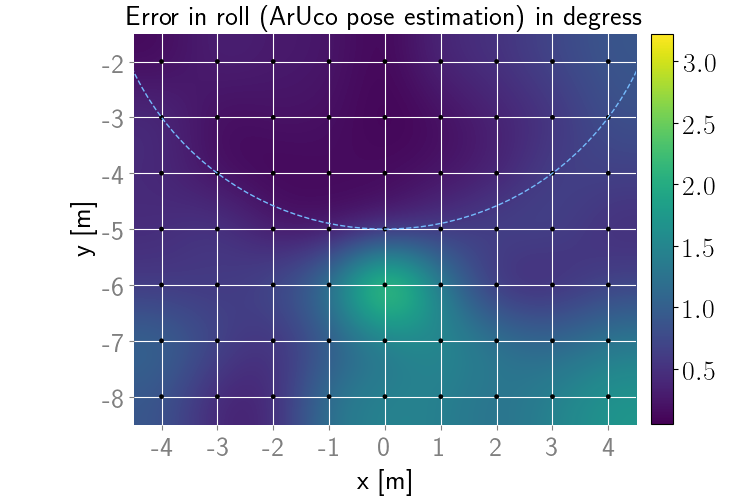
\includegraphics[width=\textwidth]{../Figures/GPS2Vision_pose_estimation_test/test2_aruco_board_width_0.3_space_0.15/aruco_pose_estimation_error_roll.png}
        \caption{}
        \label{fig:GPS2Vision_pose_estimation_test2_roll}
    \end{subfigure}
    \hspace{-0.9em}
    \begin{subfigure}[t]{.337\textwidth}
        \centering
        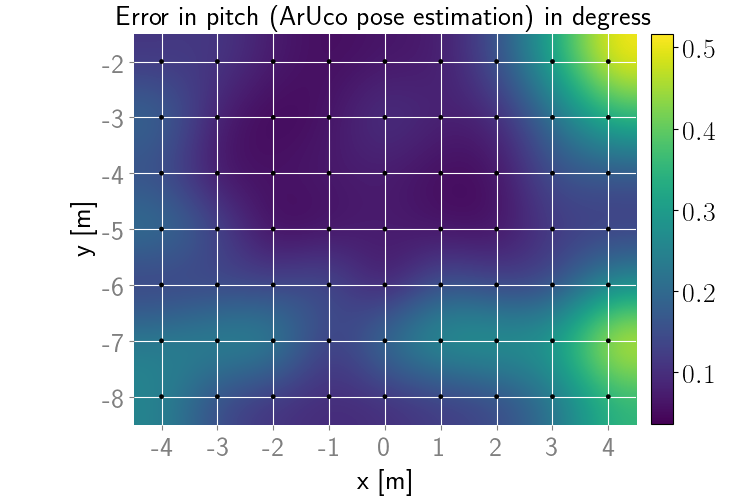
\includegraphics[width=\textwidth]{../Figures/GPS2Vision_pose_estimation_test/test2_aruco_board_width_0.3_space_0.15/aruco_pose_estimation_error_pitch.png}
        \caption{}
        \label{fig:GPS2Vision_pose_estimation_test2_pitch}
    \end{subfigure}
    \hspace{-0.9em}
    \begin{subfigure}[t]{.337\textwidth}
        \centering
        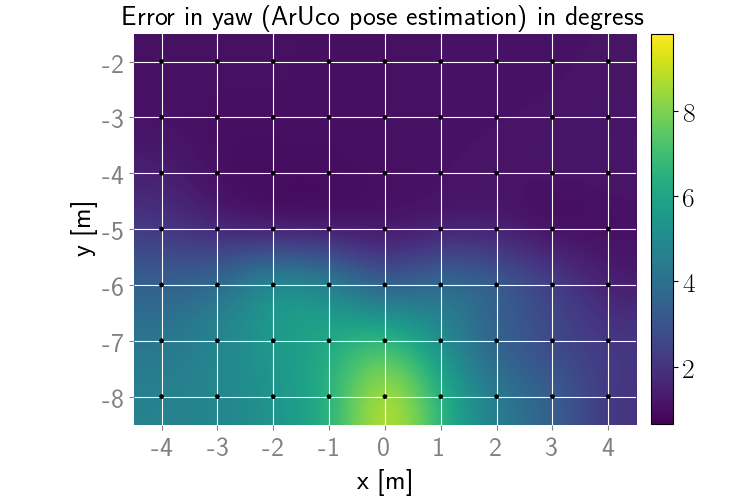
\includegraphics[width=\textwidth]{../Figures/GPS2Vision_pose_estimation_test/test2_aruco_board_width_0.3_space_0.15/aruco_pose_estimation_error_yaw.png}
        \caption{}
        \label{fig:GPS2Vision_pose_estimation_test2_error_yaw}
    \end{subfigure}
    \caption{}
    \label{fig:GPS2Vision_pose_estimation_test2_error_ori}
\end{figure}

\begin{figure}[H]
    \centering
    \begin{subfigure}[t]{.47\textwidth}
        \centering
        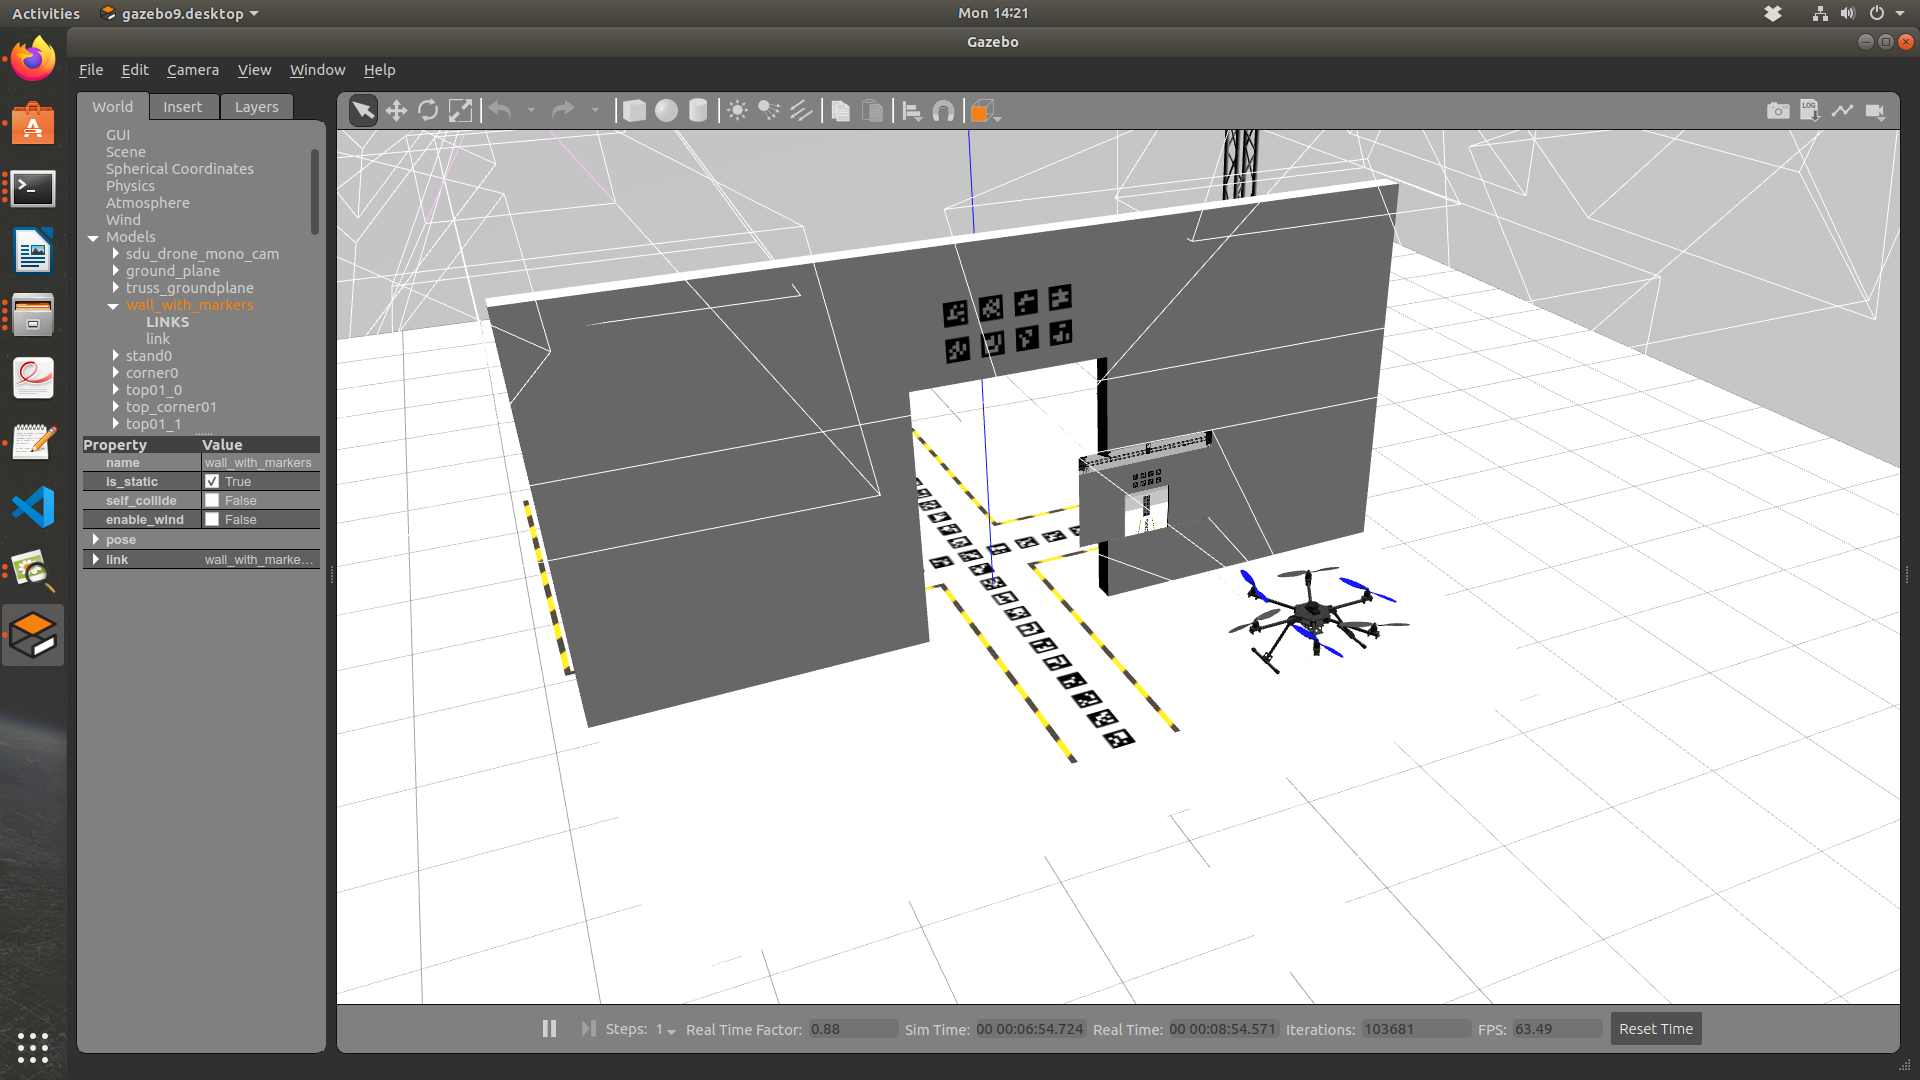
\includegraphics[width=\textwidth]{../Figures/analyse_rolling_average/optimal_pose.png}
        \caption{}
        \label{fig:GPS2Vision_pose_estimation_test2_roll}
    \end{subfigure}
    \hspace{0.5em}
    \begin{subfigure}[t]{.47\textwidth}
        \centering
        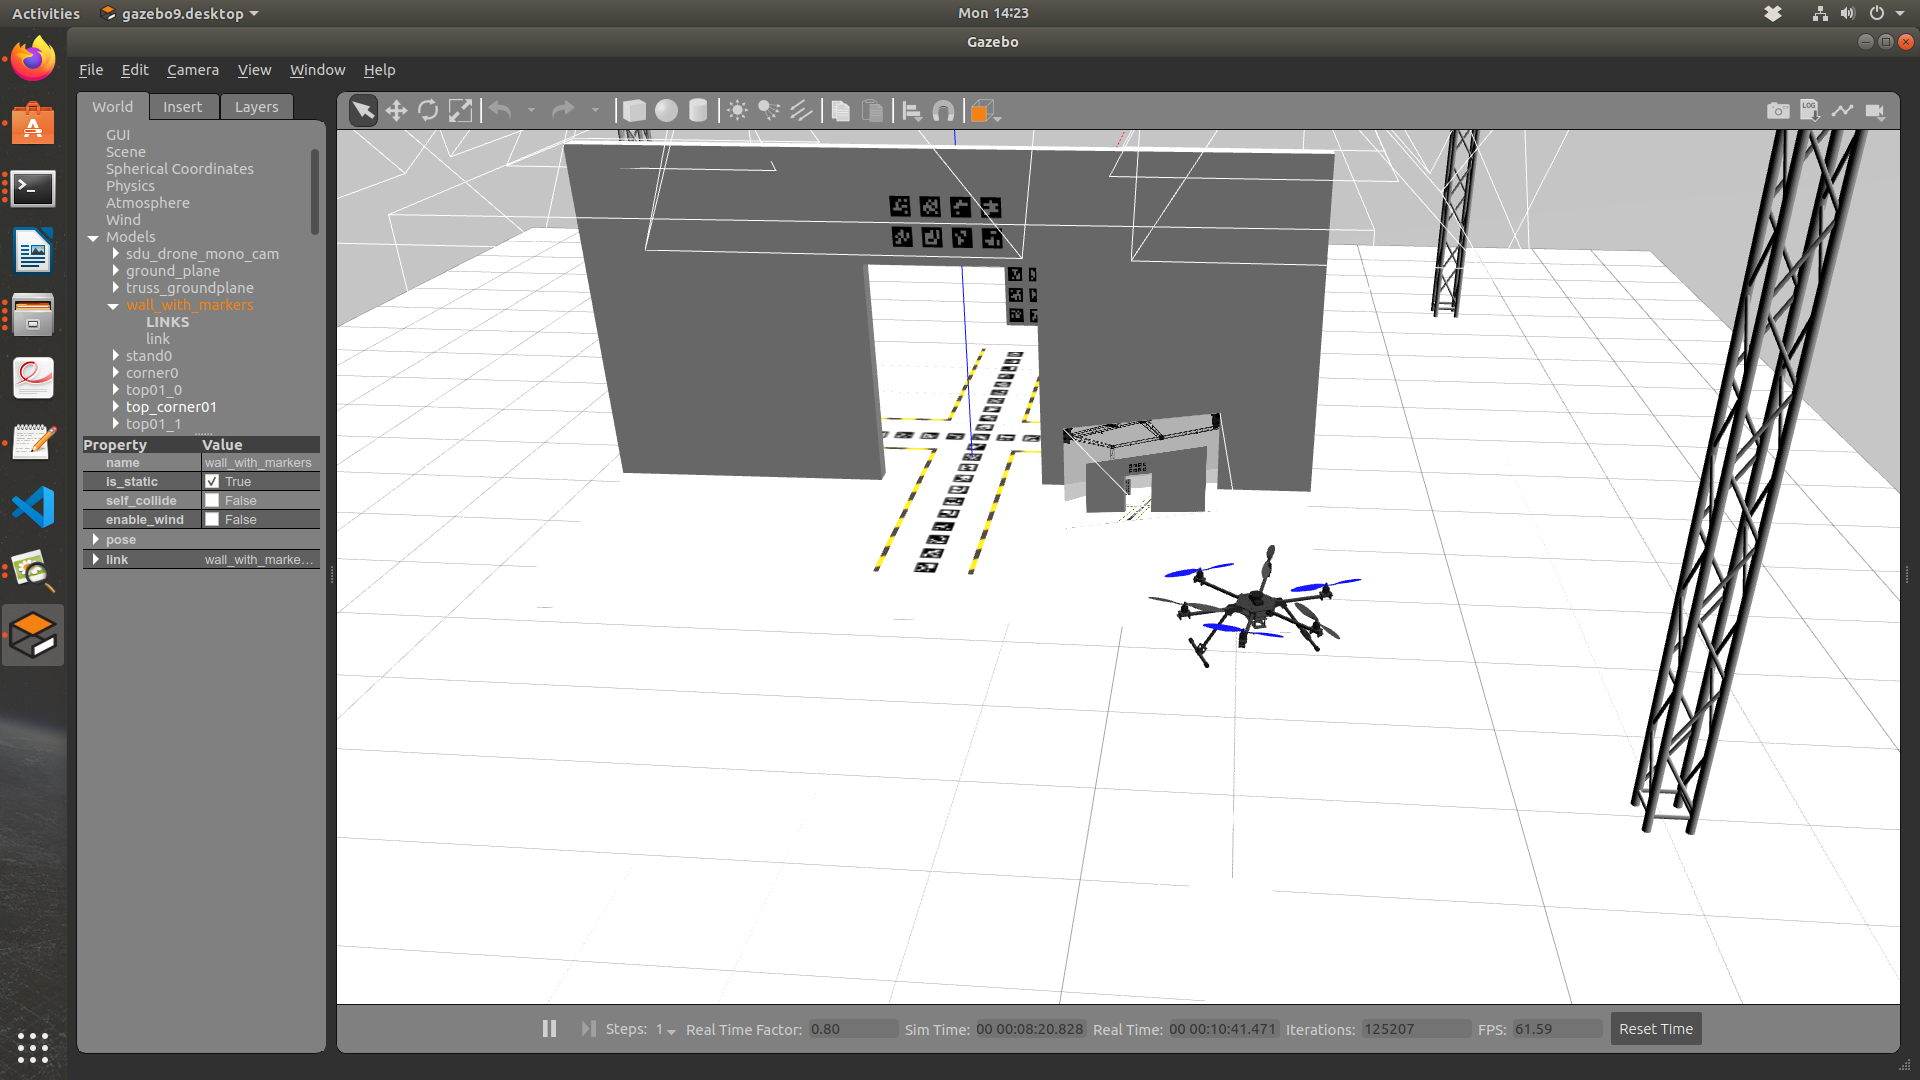
\includegraphics[width=\textwidth]{../Figures/analyse_rolling_average/bad_pose.png}
        \caption{}
        \label{fig:GPS2Vision_pose_estimation_test2_pitch}
    \end{subfigure}
    \caption{}
    \label{fig:GPS2Vision_pose_estimation_test2_error_ori}
\end{figure}

\begin{figure}[H]
    \centering
    \begin{subfigure}[t]{.30\textwidth}
        \centering
        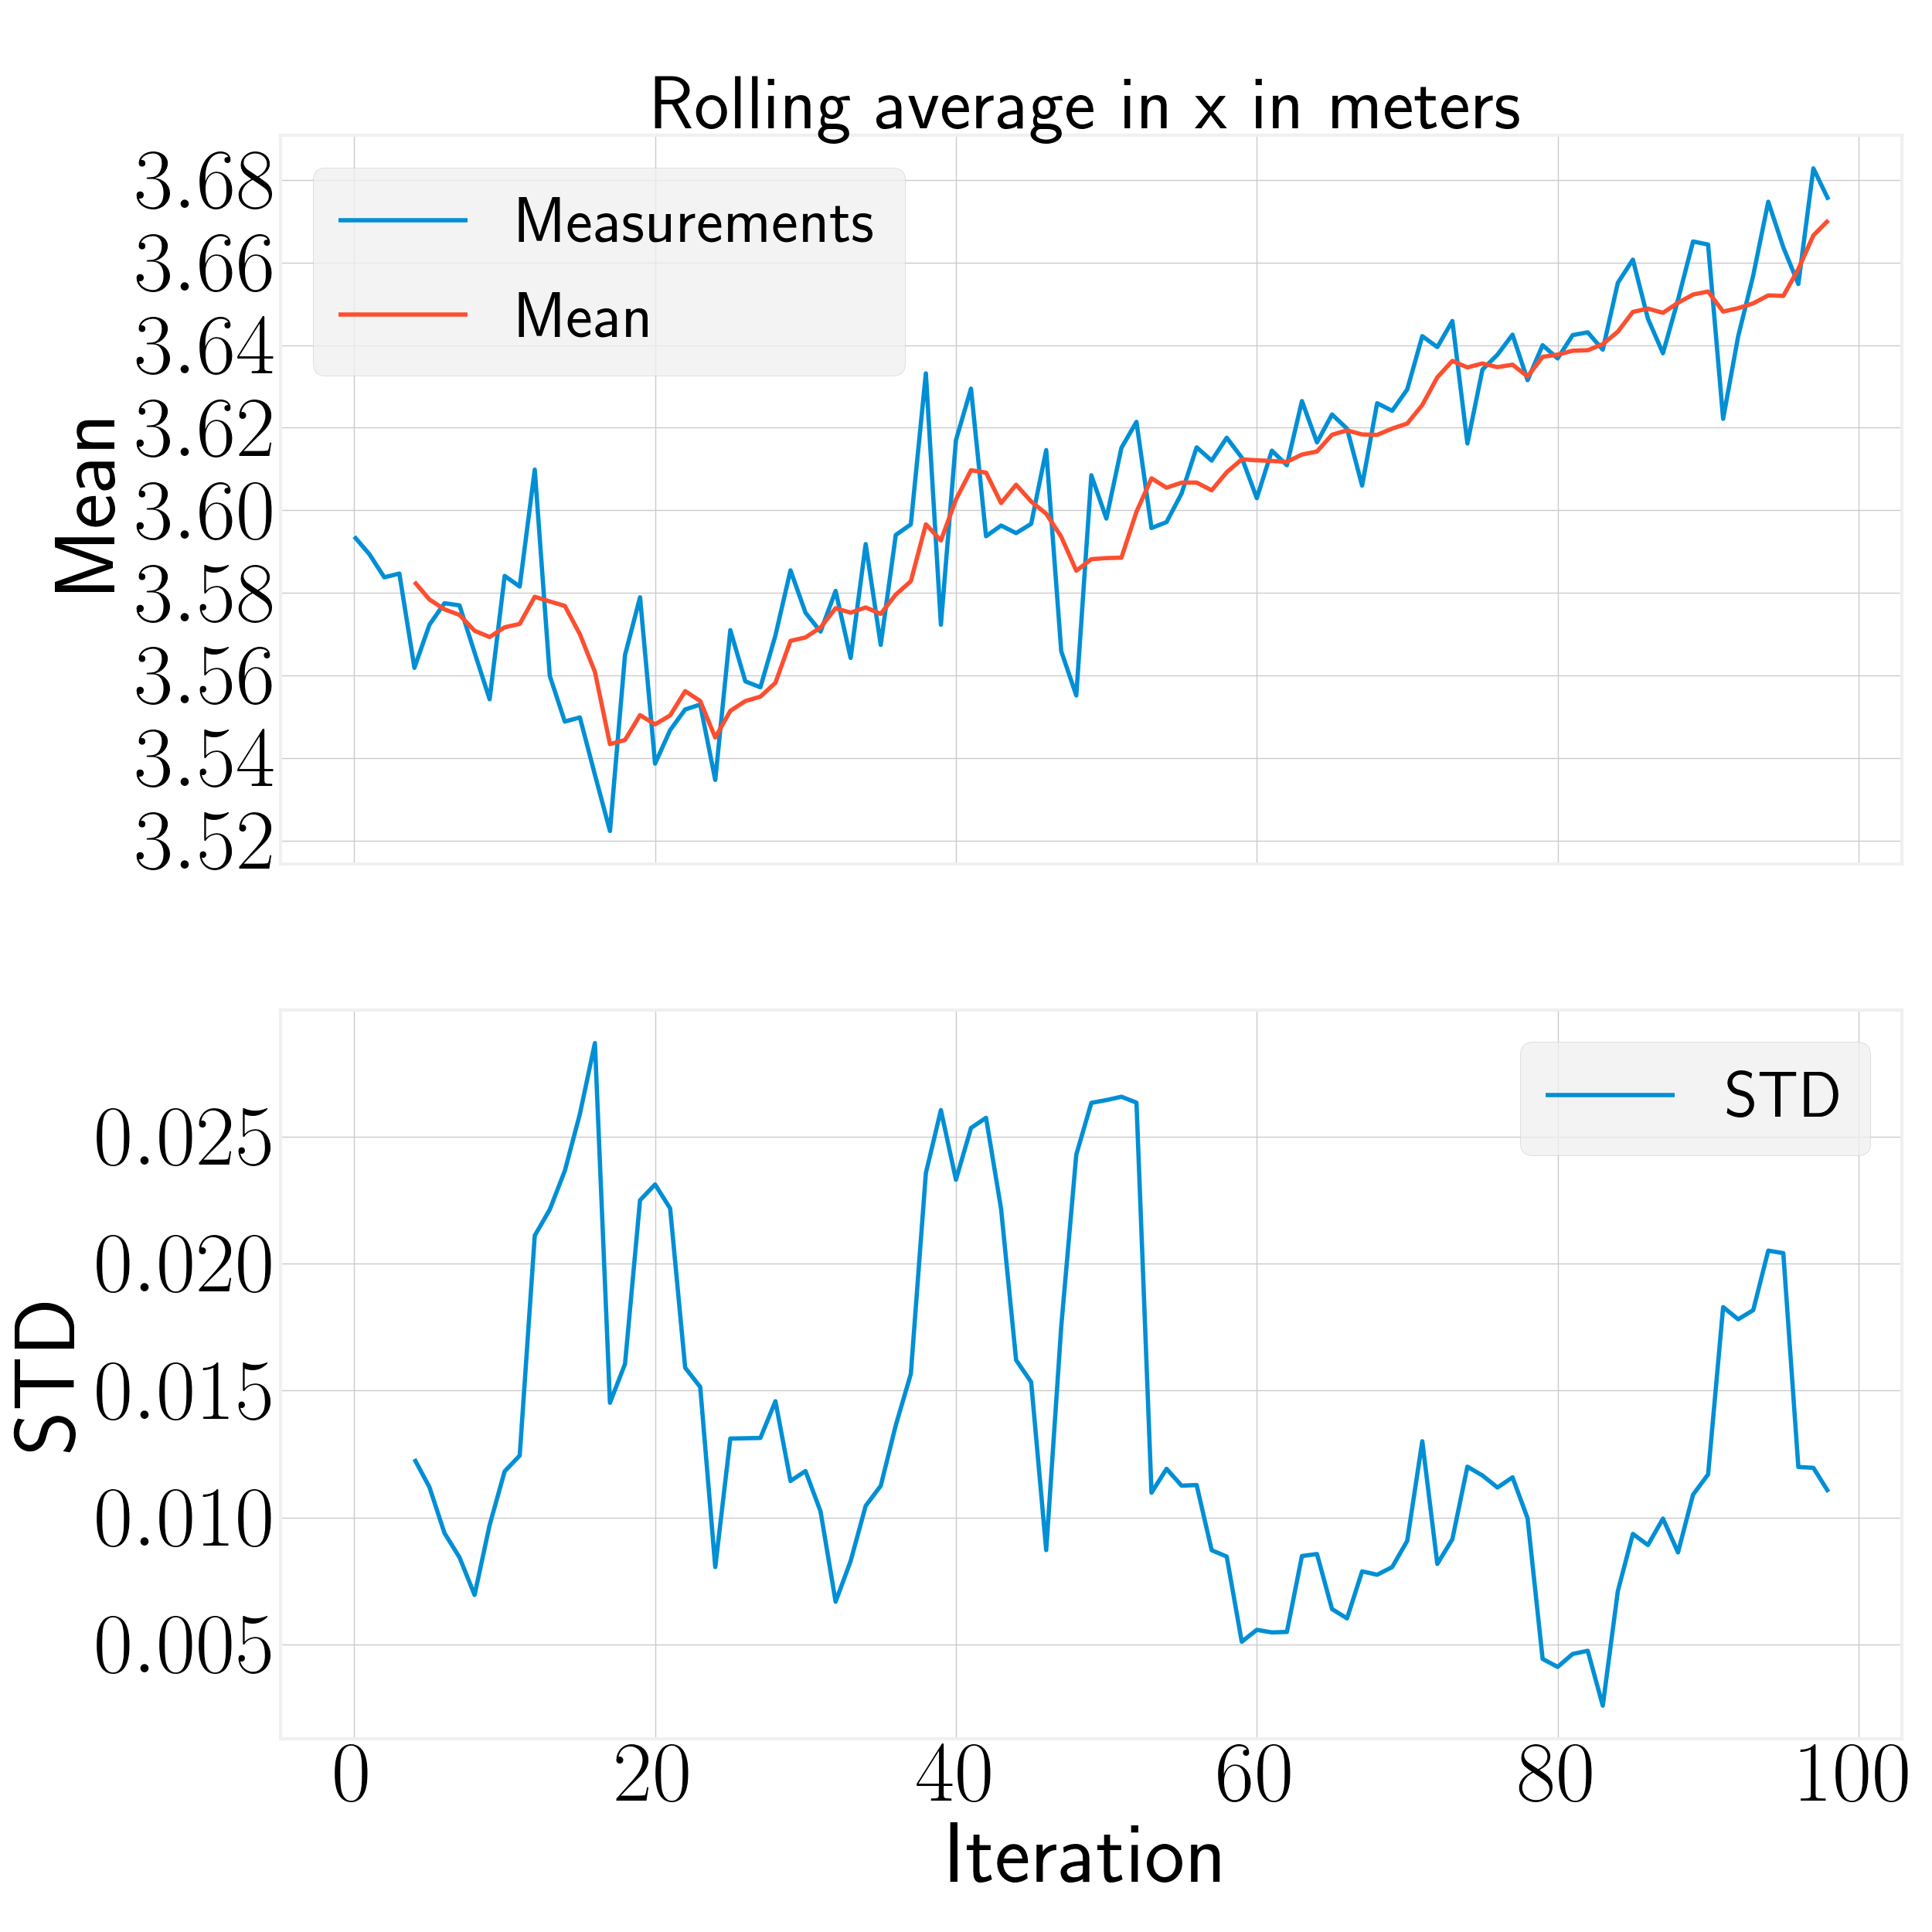
\includegraphics[width=\textwidth]{../Figures/analyse_rolling_average/test1/Calculated_rolling_average_in_x_with_mean_and_STD.png}
        \caption{}
        \label{fig:rolling_average_in_x_test1}
    \end{subfigure}
     \hspace{0.2em}
    \begin{subfigure}[t]{.30\textwidth}
        \centering
        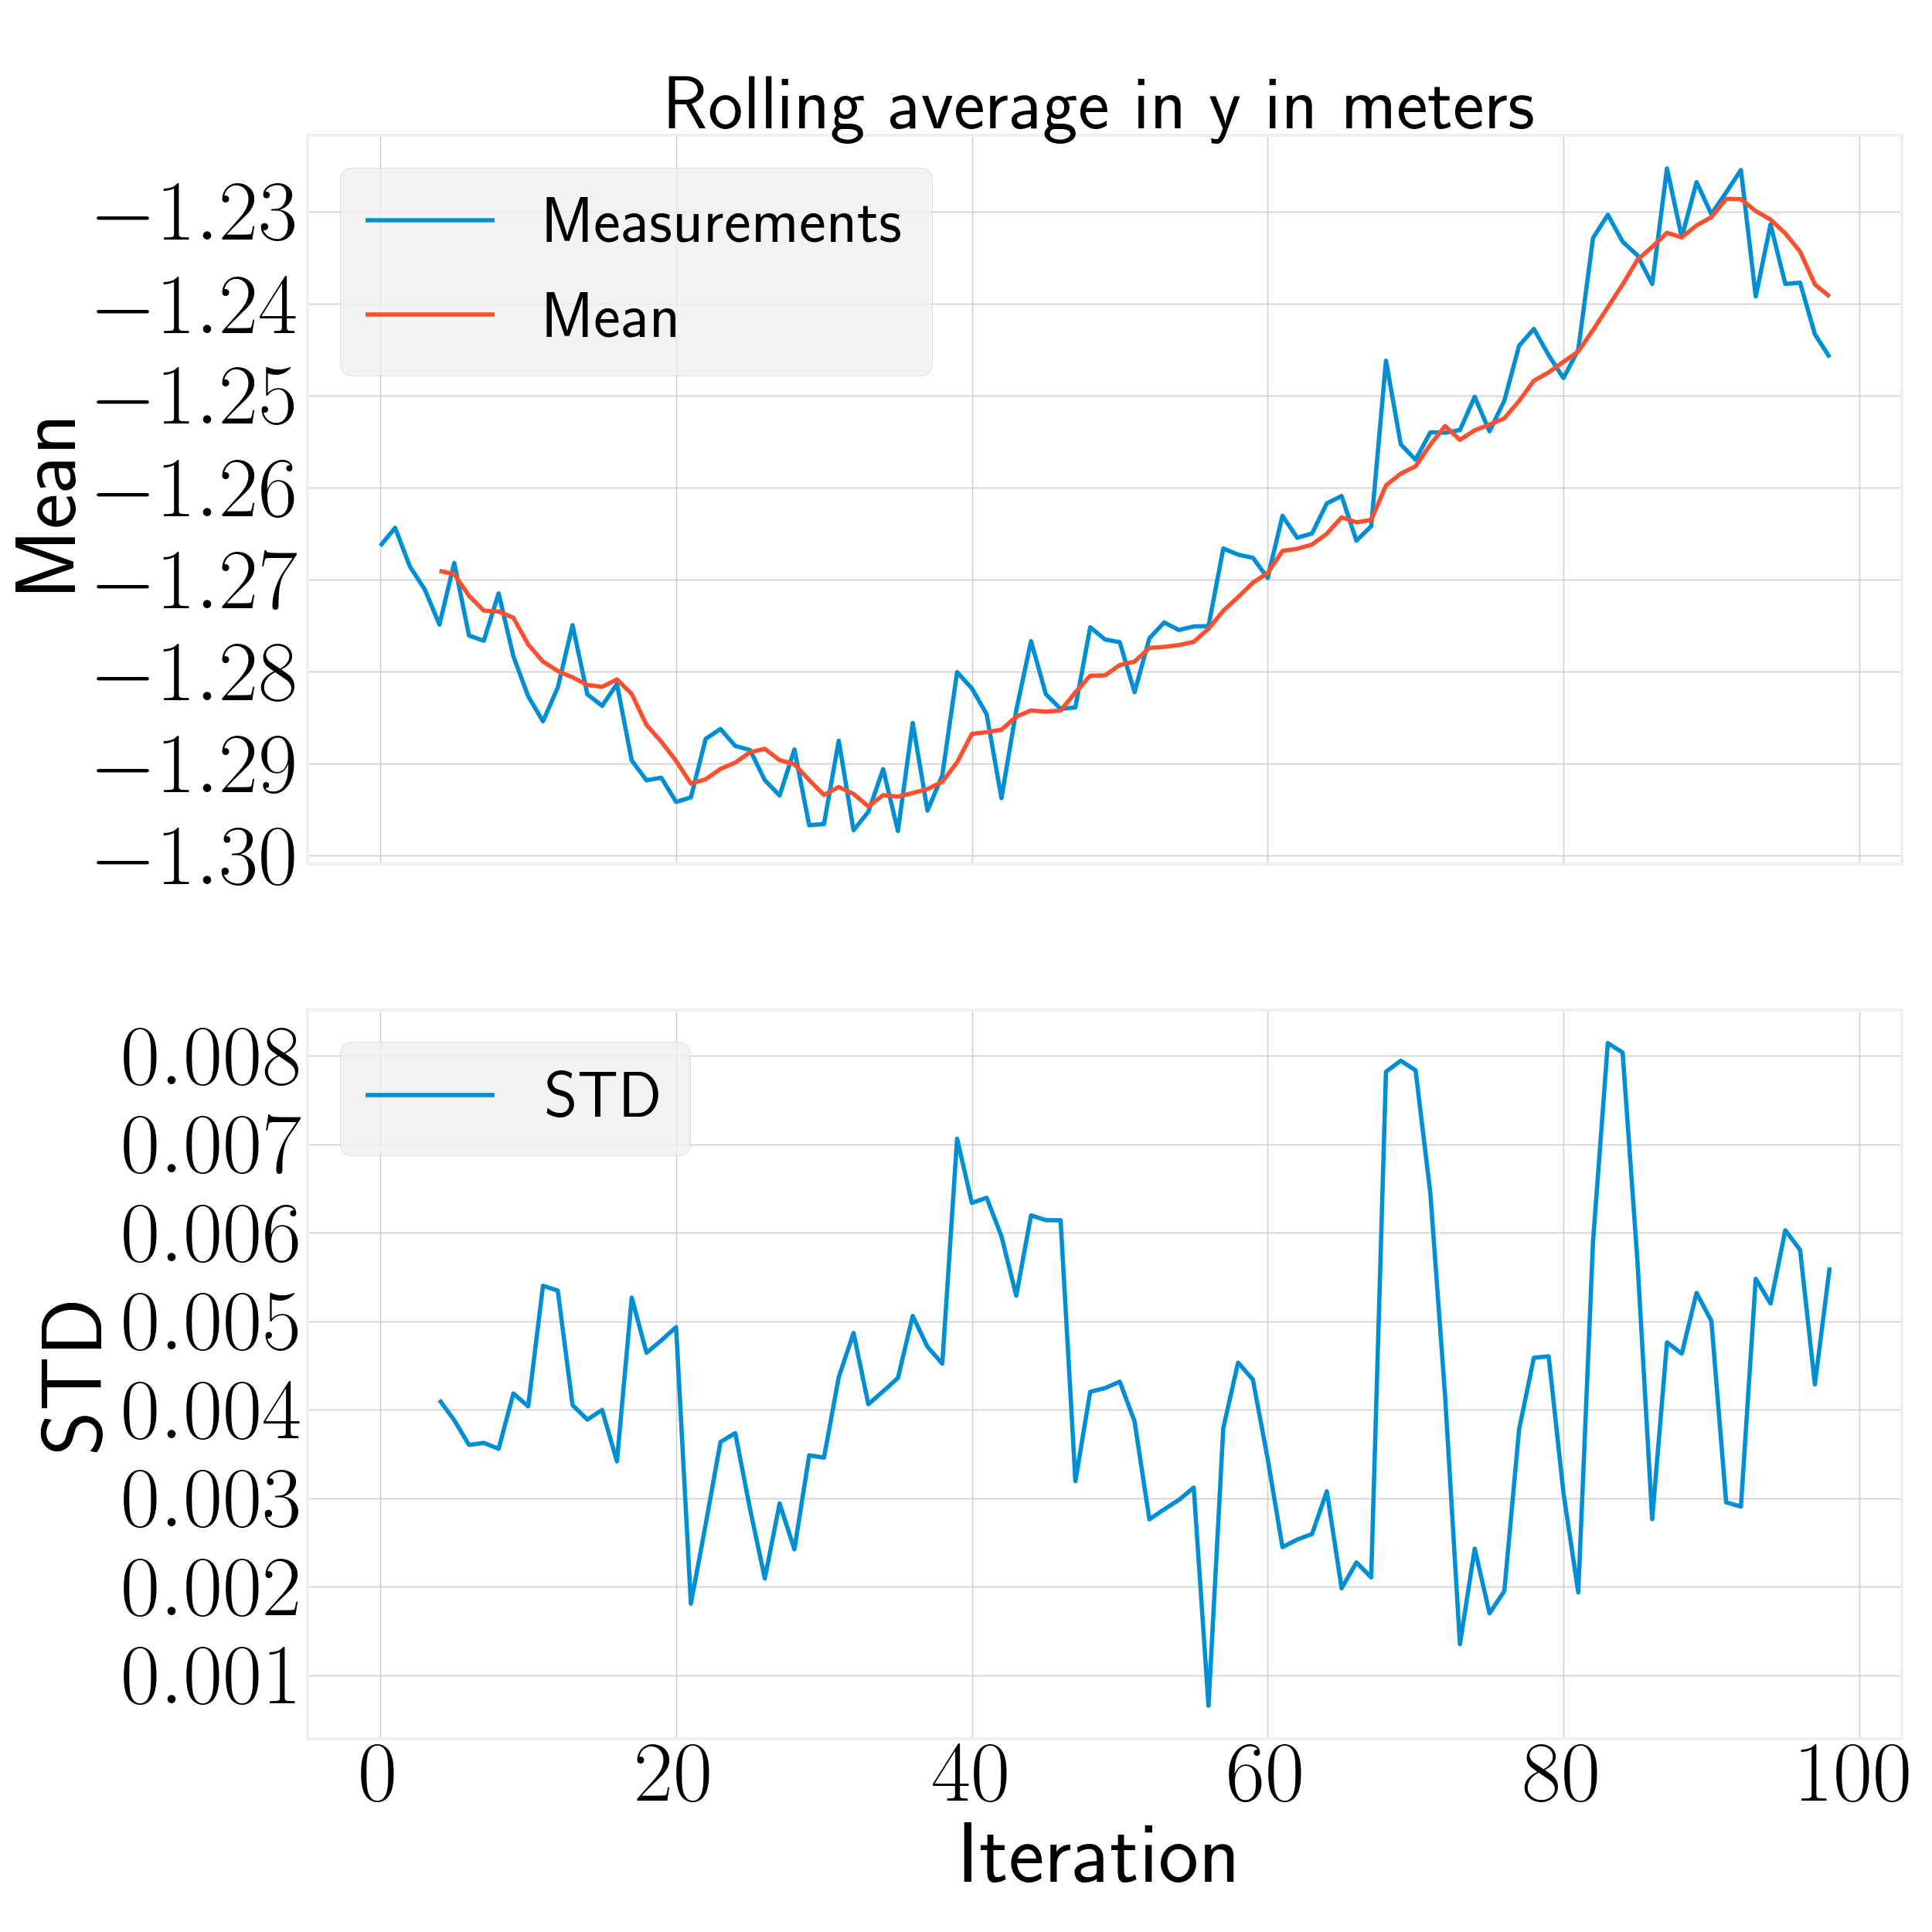
\includegraphics[width=\textwidth]{../Figures/analyse_rolling_average/test1/Calculated_rolling_average_in_y_with_mean_and_STD.png}
        \caption{}
        \label{fig:rolling_average_in_y_test1}
    \end{subfigure}
     \hspace{0.2em}
    \begin{subfigure}[t]{.30\textwidth}
        \centering
        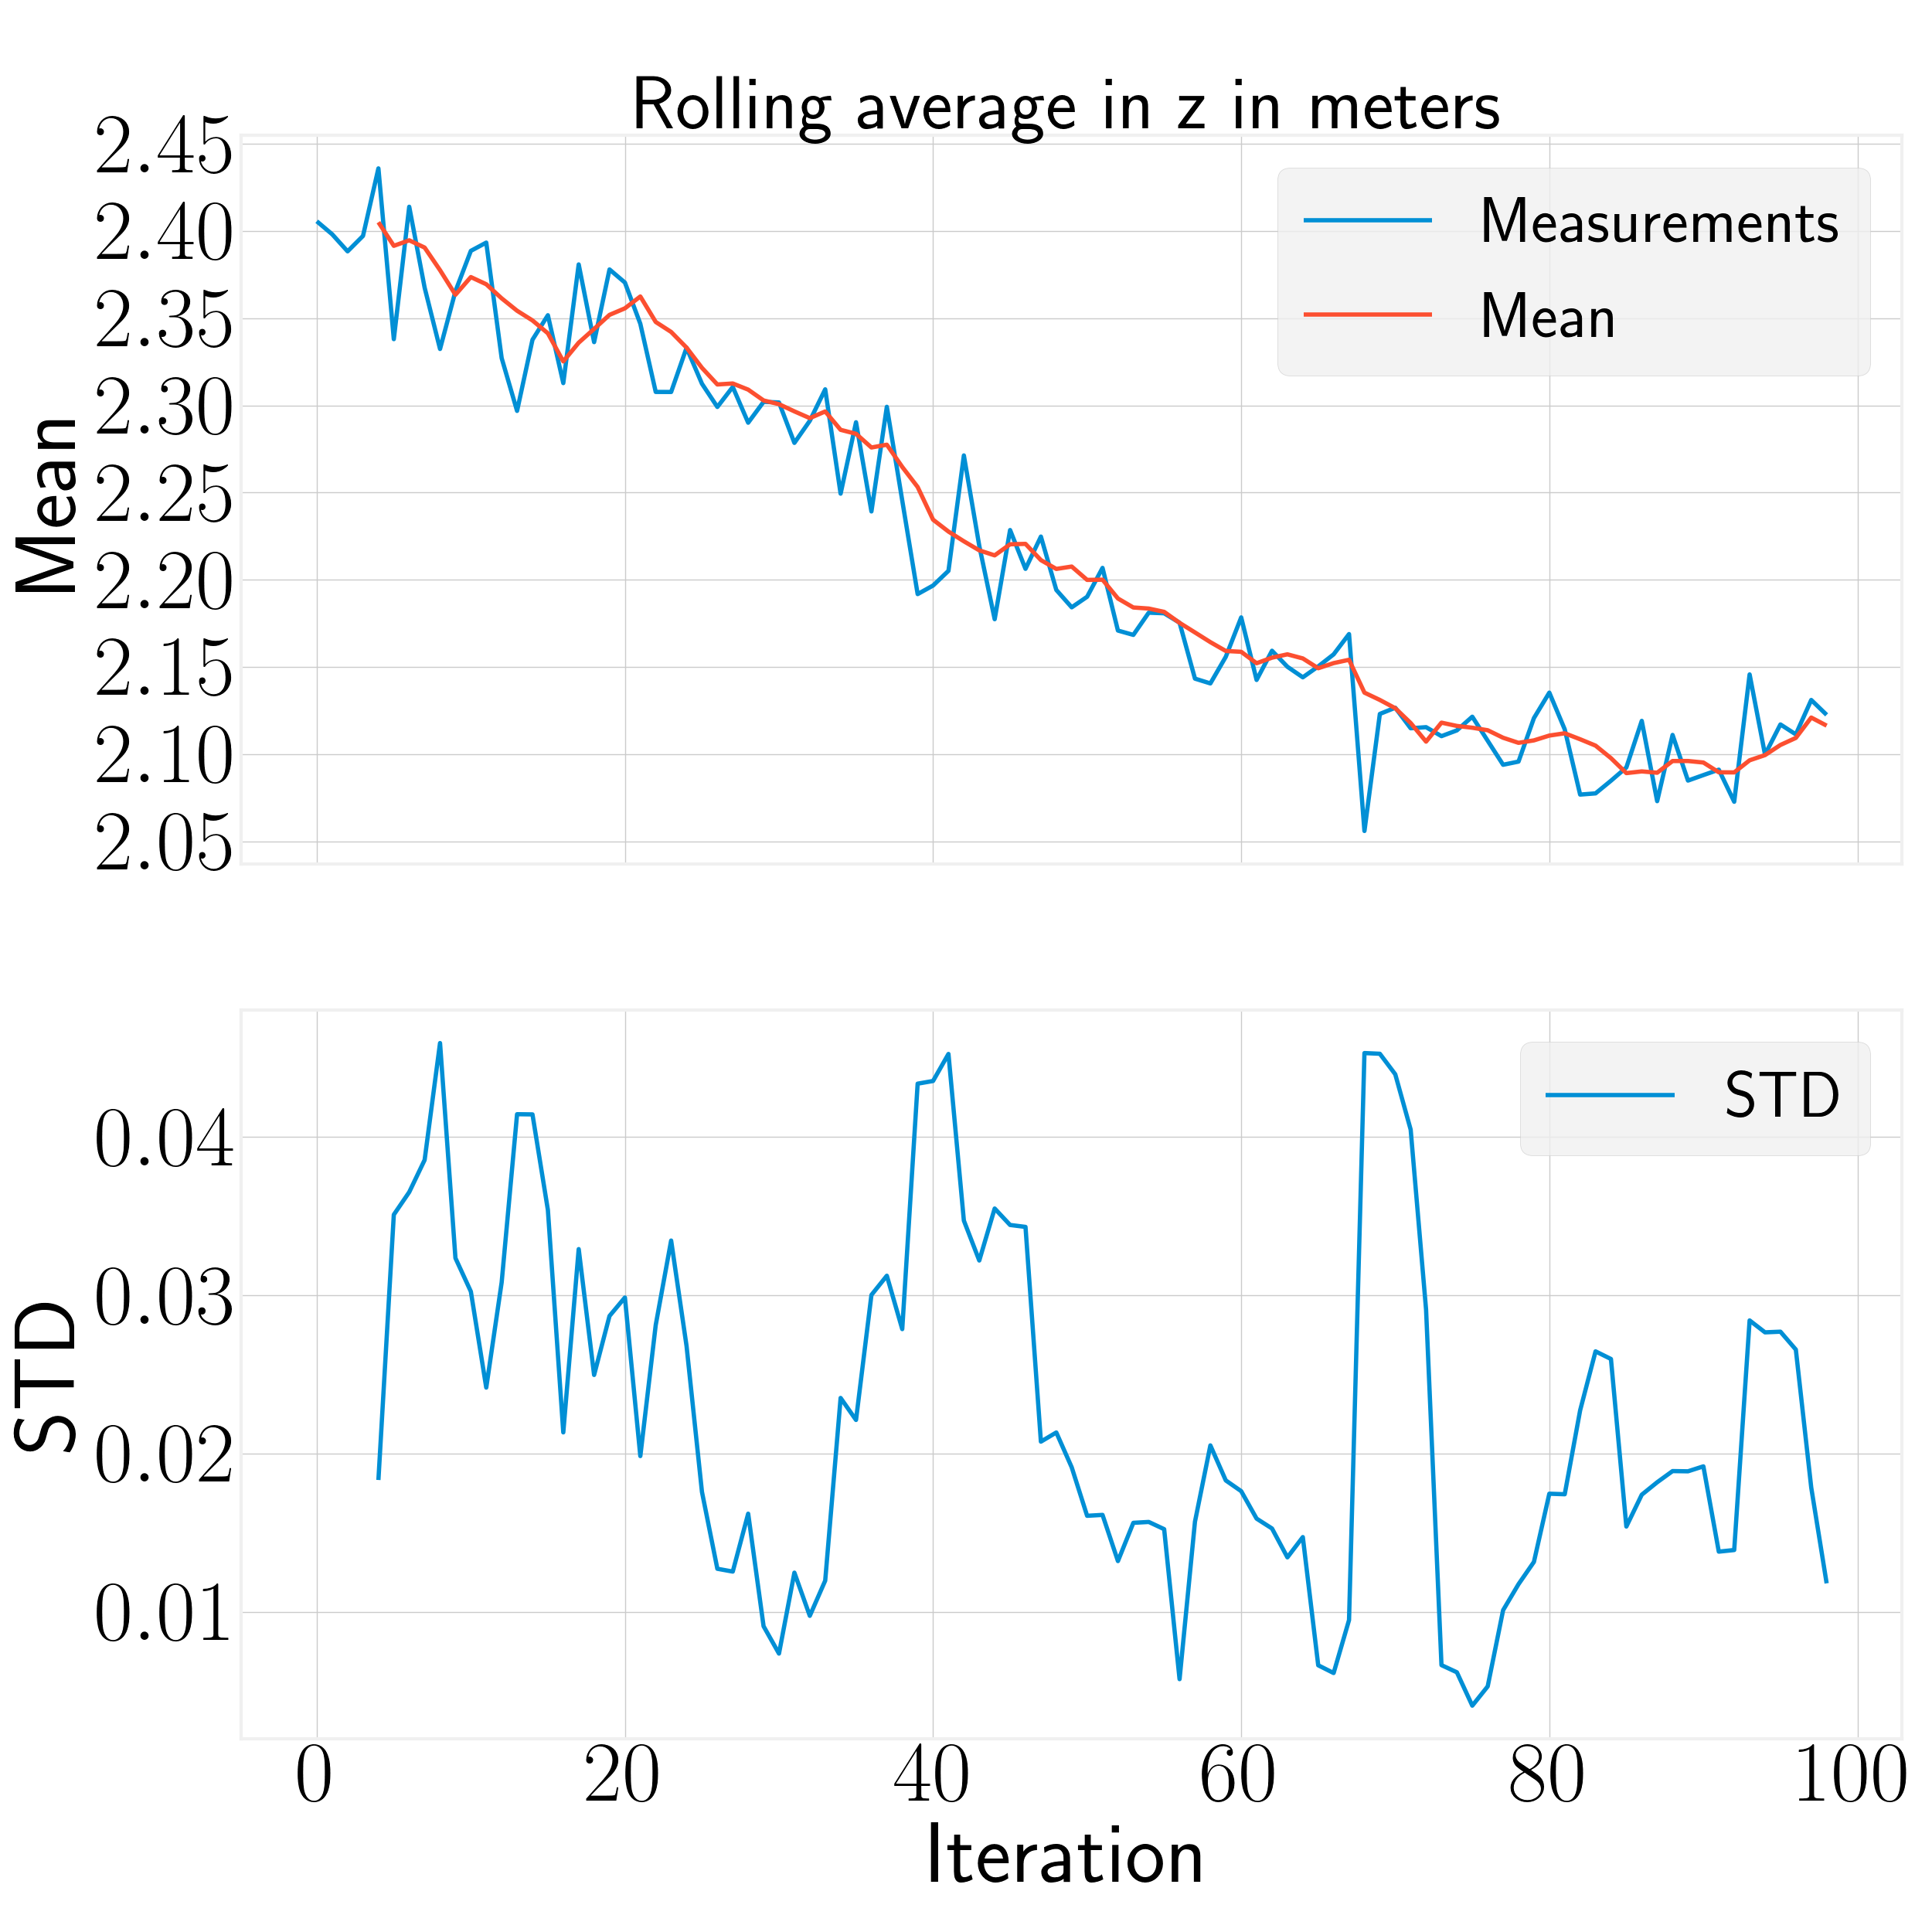
\includegraphics[width=\textwidth]{../Figures/analyse_rolling_average/test1/Calculated_rolling_average_in_z_with_mean_and_STD.png}
        \caption{}
        \label{fig:rolling_average_in_z_test1}
    \end{subfigure}
    \caption{}
    \label{fig:rolling_average_pos_test1}
\end{figure}

\begin{figure}[H]
    \centering
    \begin{subfigure}[t]{.30\textwidth}
        \centering
        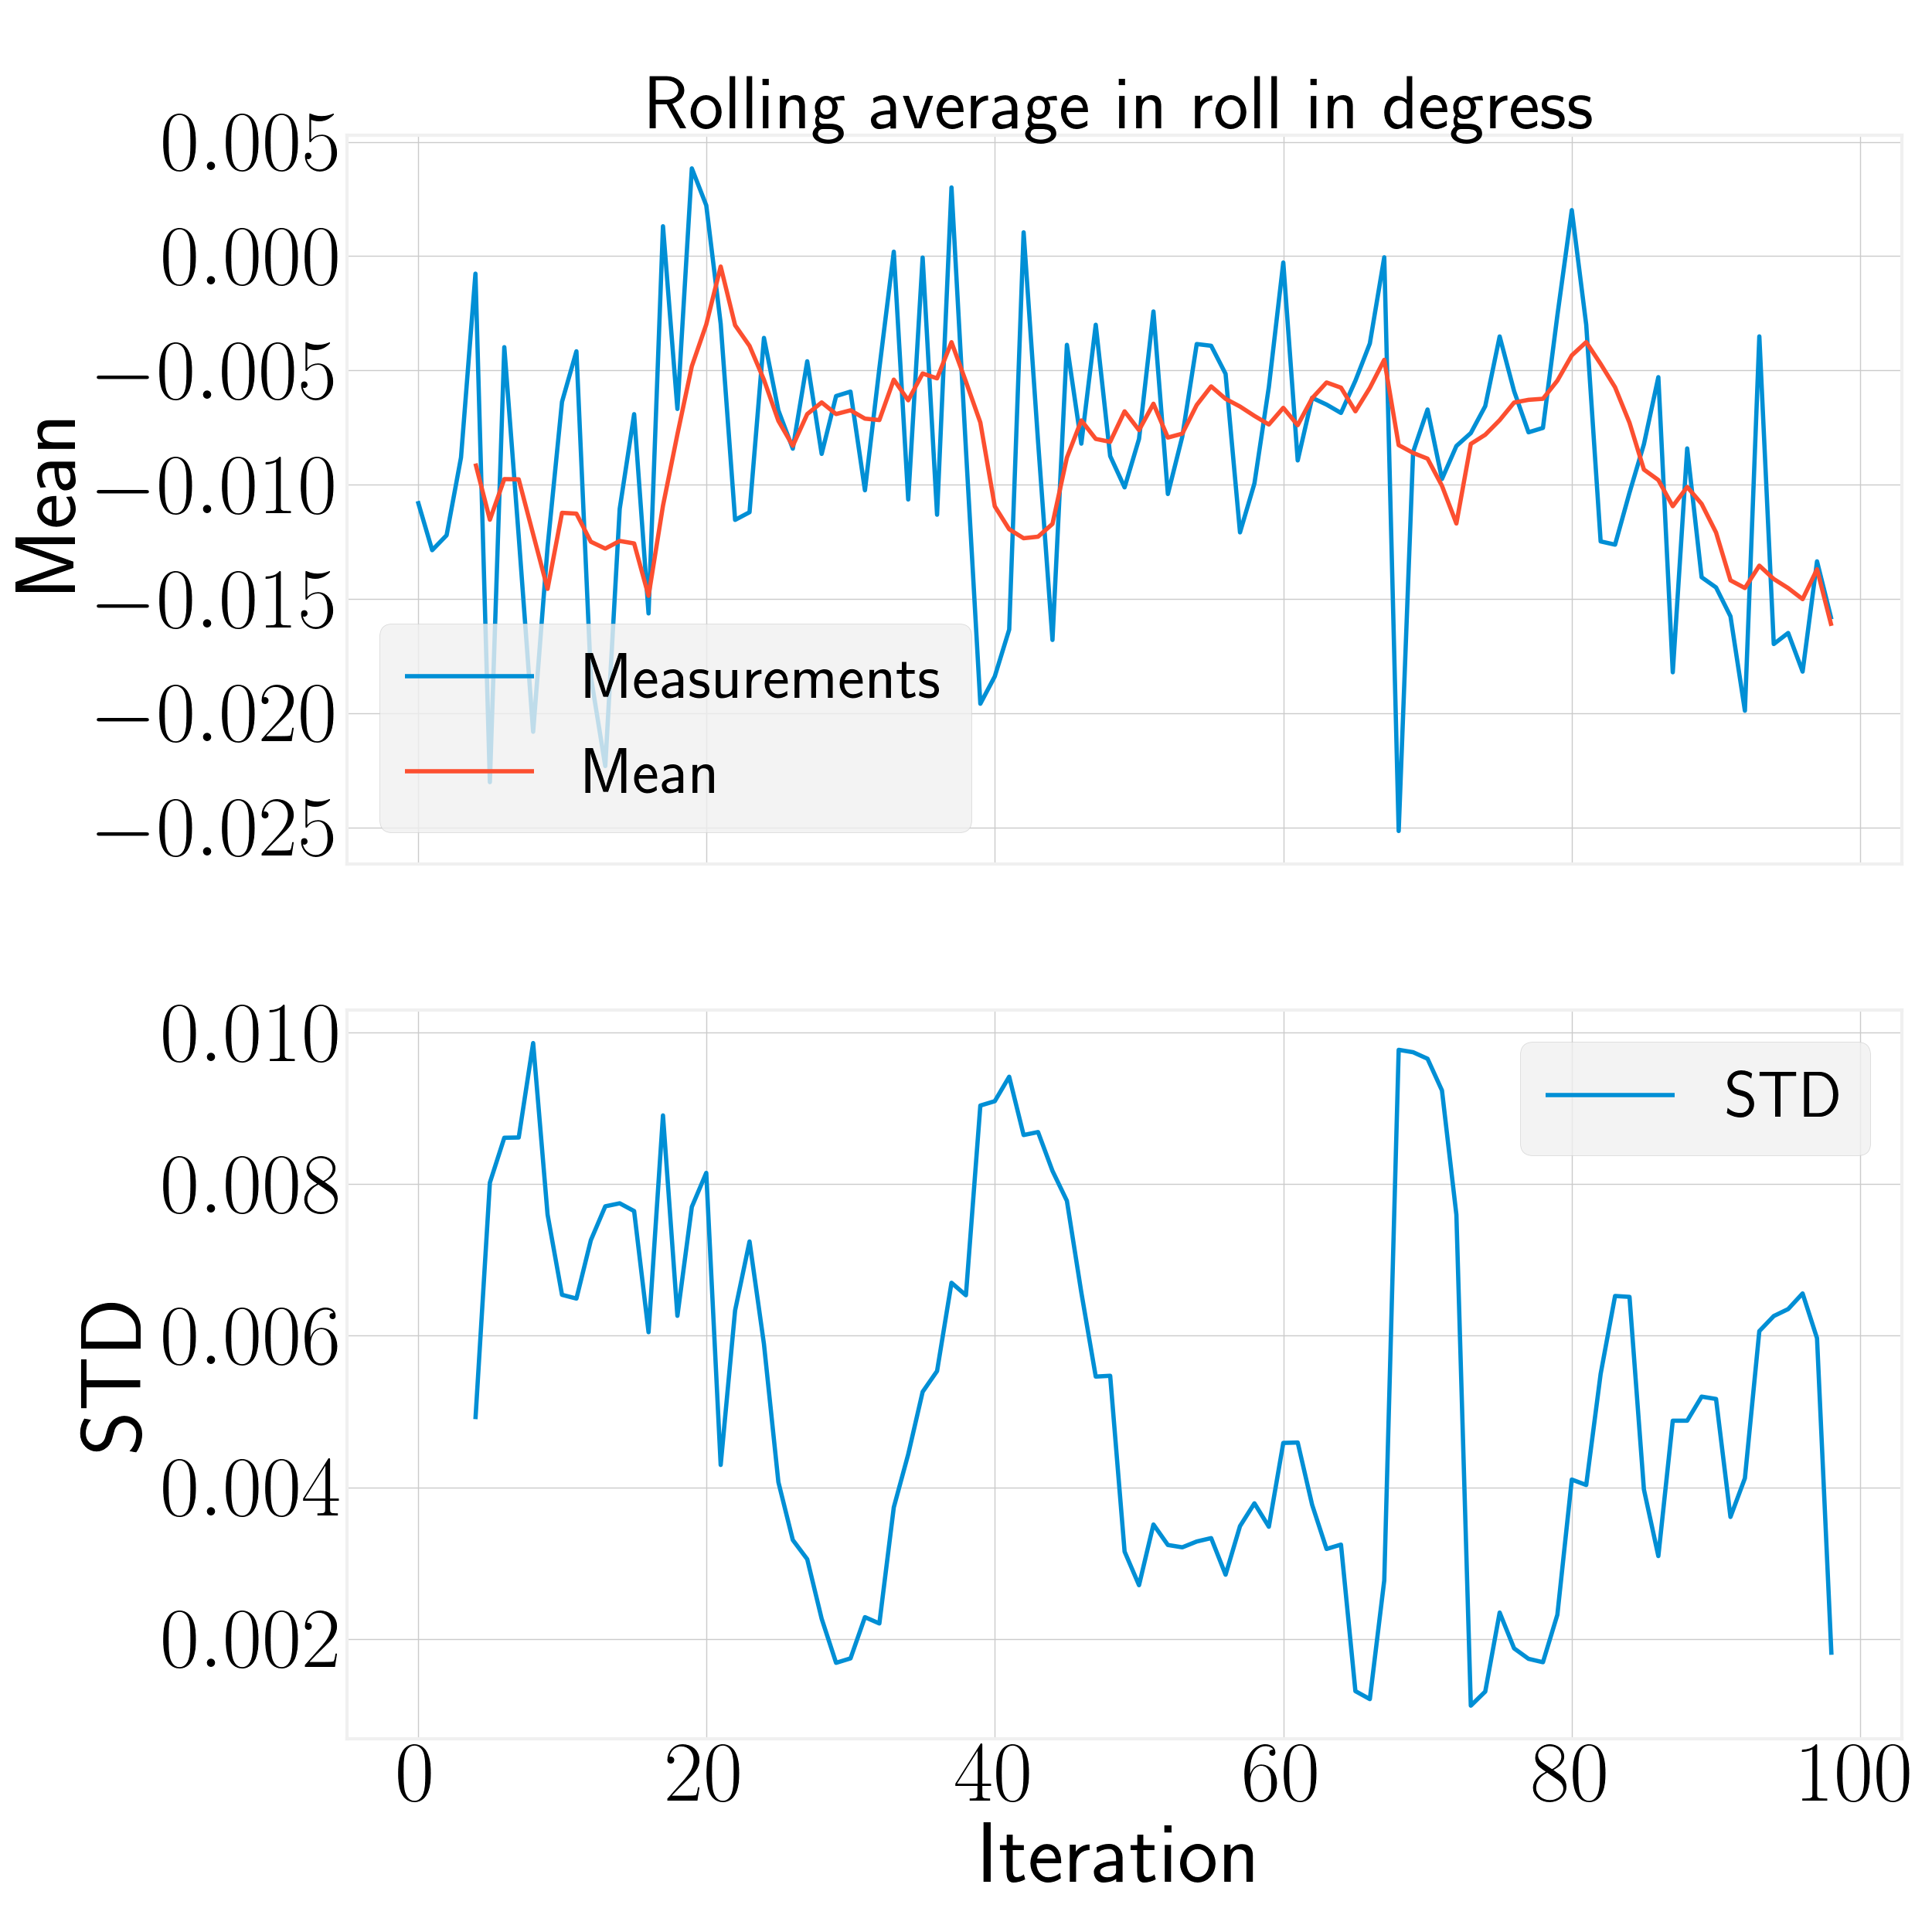
\includegraphics[width=\textwidth]{../Figures/analyse_rolling_average/test1/Calculated_rolling_average_in_roll_with_mean_and_STD.png}
        \caption{}
        \label{fig:rolling_average_in_roll_test1}
    \end{subfigure}
     \hspace{0.2em}
    \begin{subfigure}[t]{.30\textwidth}
        \centering
        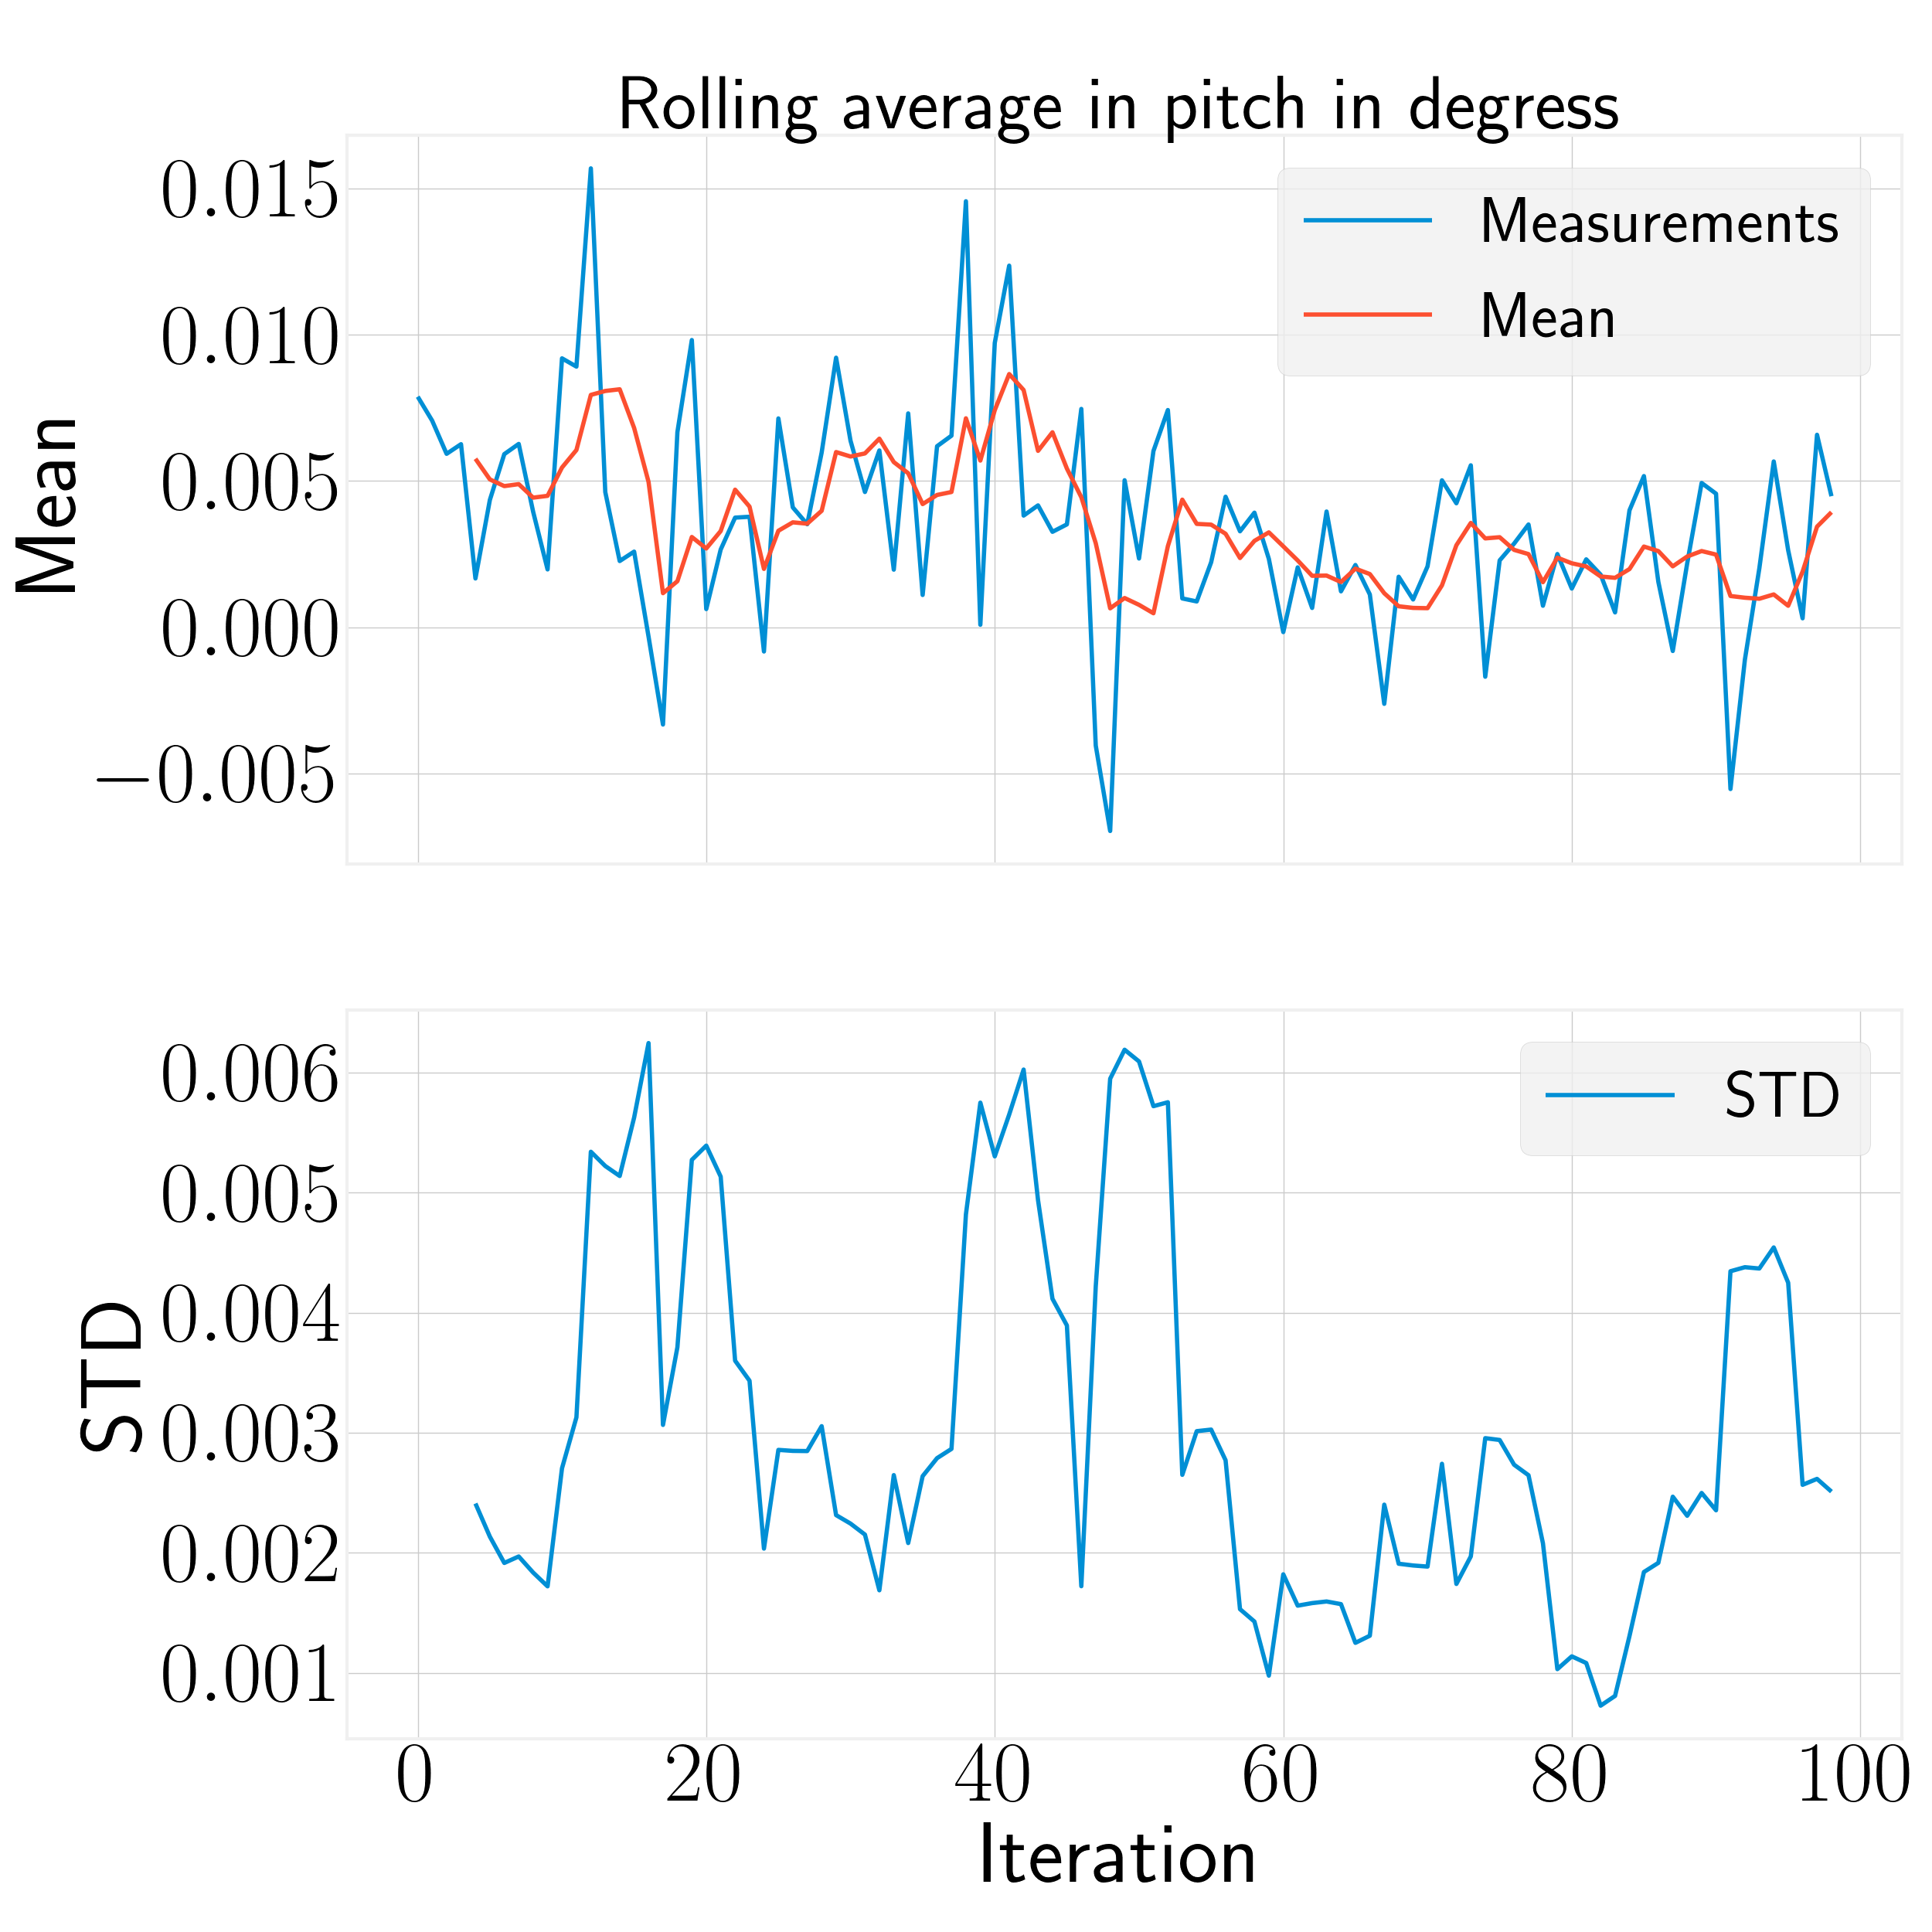
\includegraphics[width=\textwidth]{../Figures/analyse_rolling_average/test1/Calculated_rolling_average_in_pitch_with_mean_and_STD.png}
        \caption{}
        \label{fig:rolling_average_in_pitch_test1}
    \end{subfigure}
     \hspace{0.2em}
    \begin{subfigure}[t]{.30\textwidth}
        \centering
        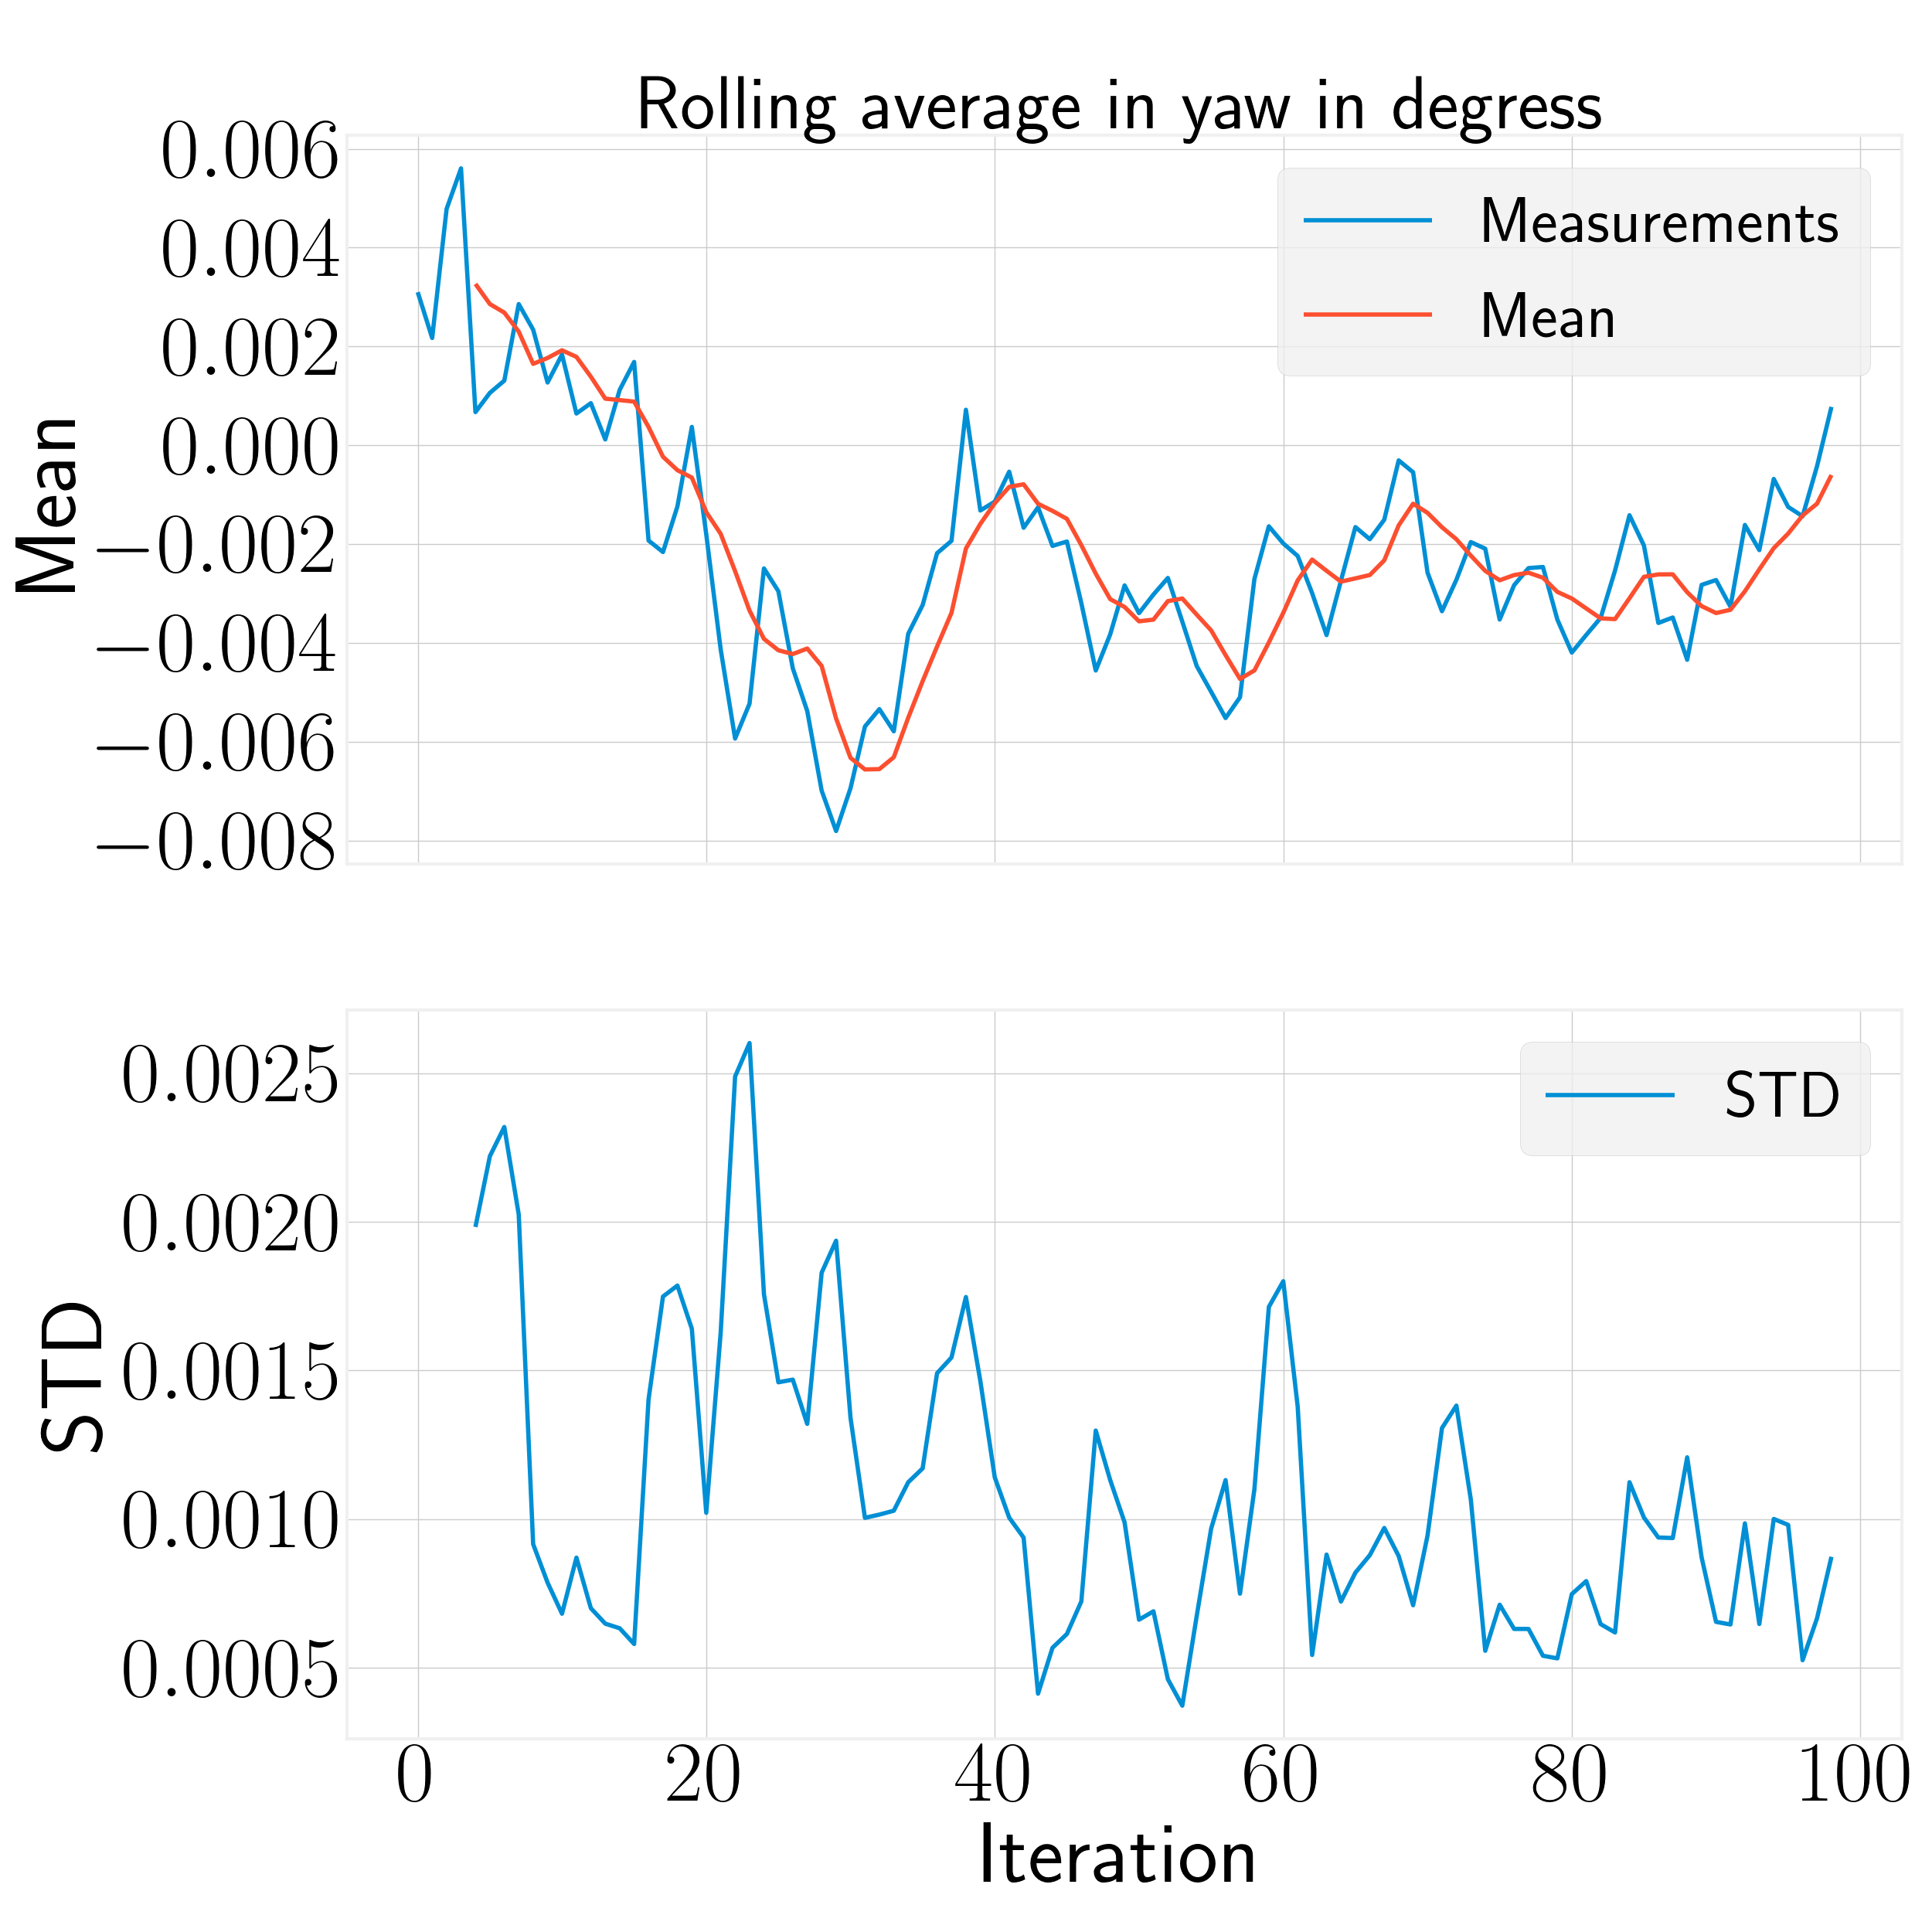
\includegraphics[width=\textwidth]{../Figures/analyse_rolling_average/test1/Calculated_rolling_average_in_yaw_with_mean_and_STD.png}
        \caption{}
        \label{fig:rolling_average_in_yaw_test1}
    \end{subfigure}
    \caption{}
    \label{fig:rolling_average_angle_test1}
\end{figure}

\begin{figure}[H]
    \centering
    \begin{subfigure}[t]{.30\textwidth}
        \centering
        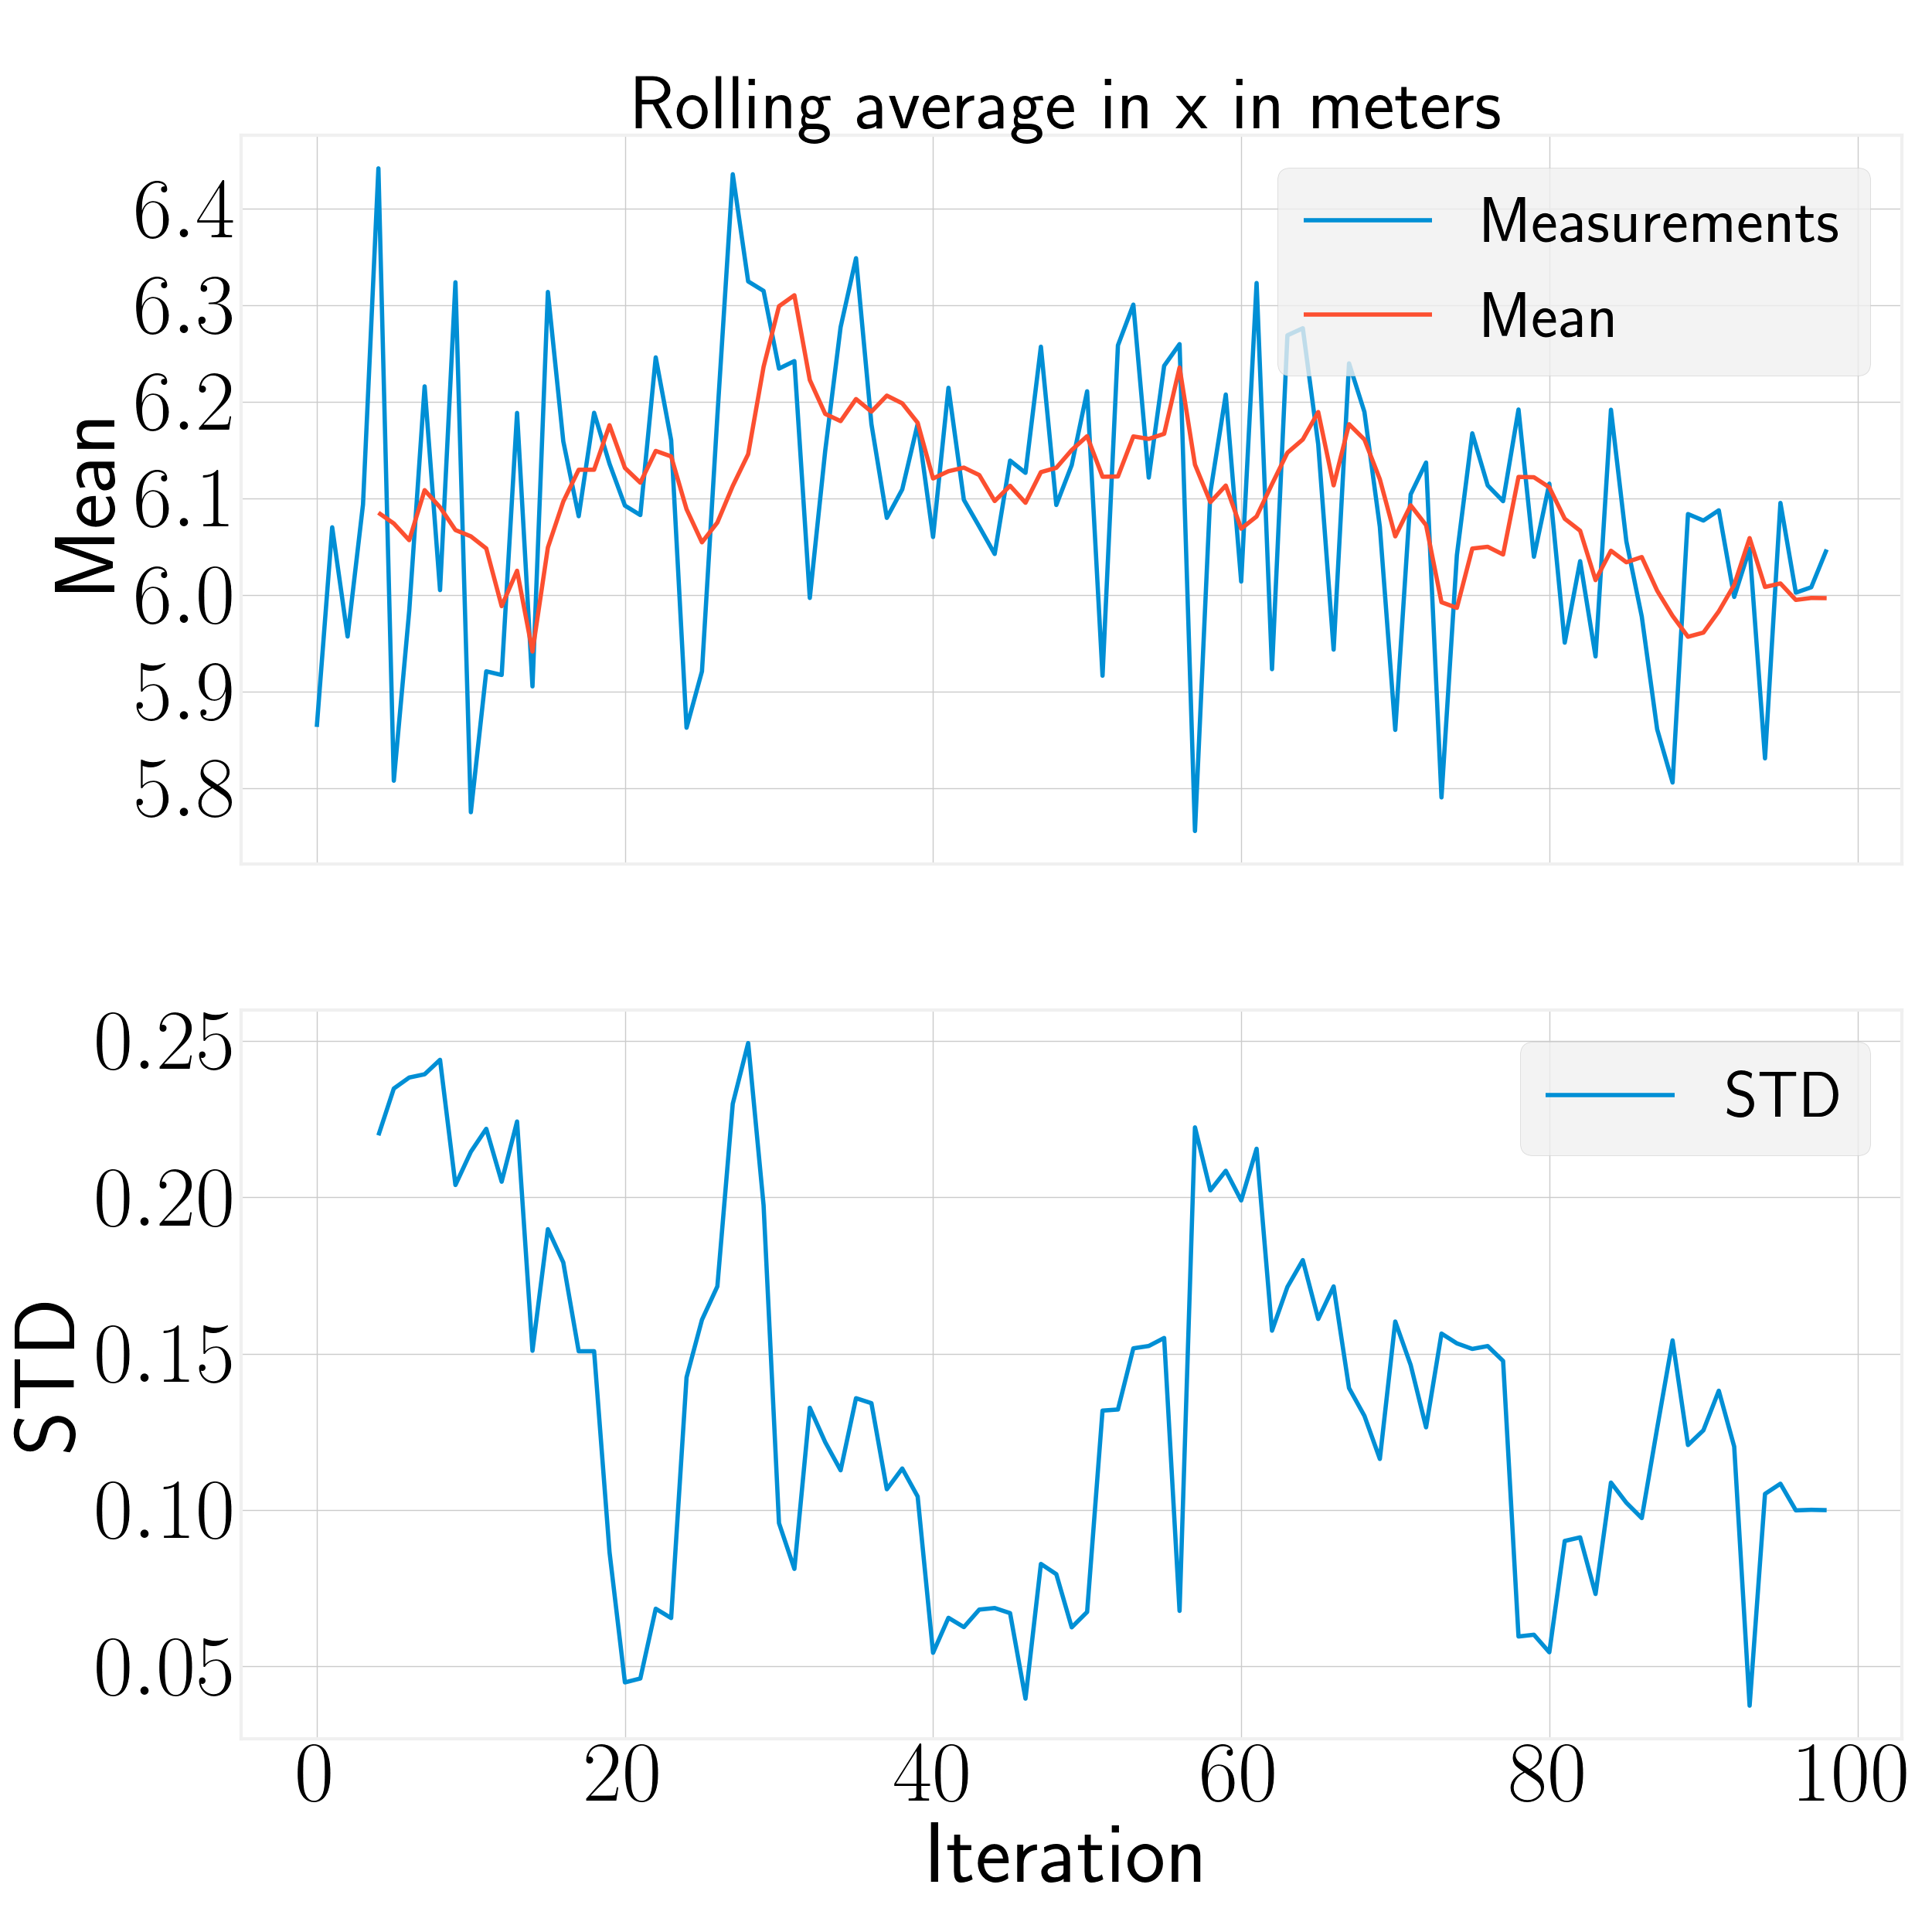
\includegraphics[width=\textwidth]{../Figures/analyse_rolling_average/test2/Calculated_rolling_average_in_x_with_mean_and_STD.png}
        \caption{}
        \label{fig:rolling_average_in_x_test2}
    \end{subfigure}
     \hspace{0.2em}
    \begin{subfigure}[t]{.30\textwidth}
        \centering
        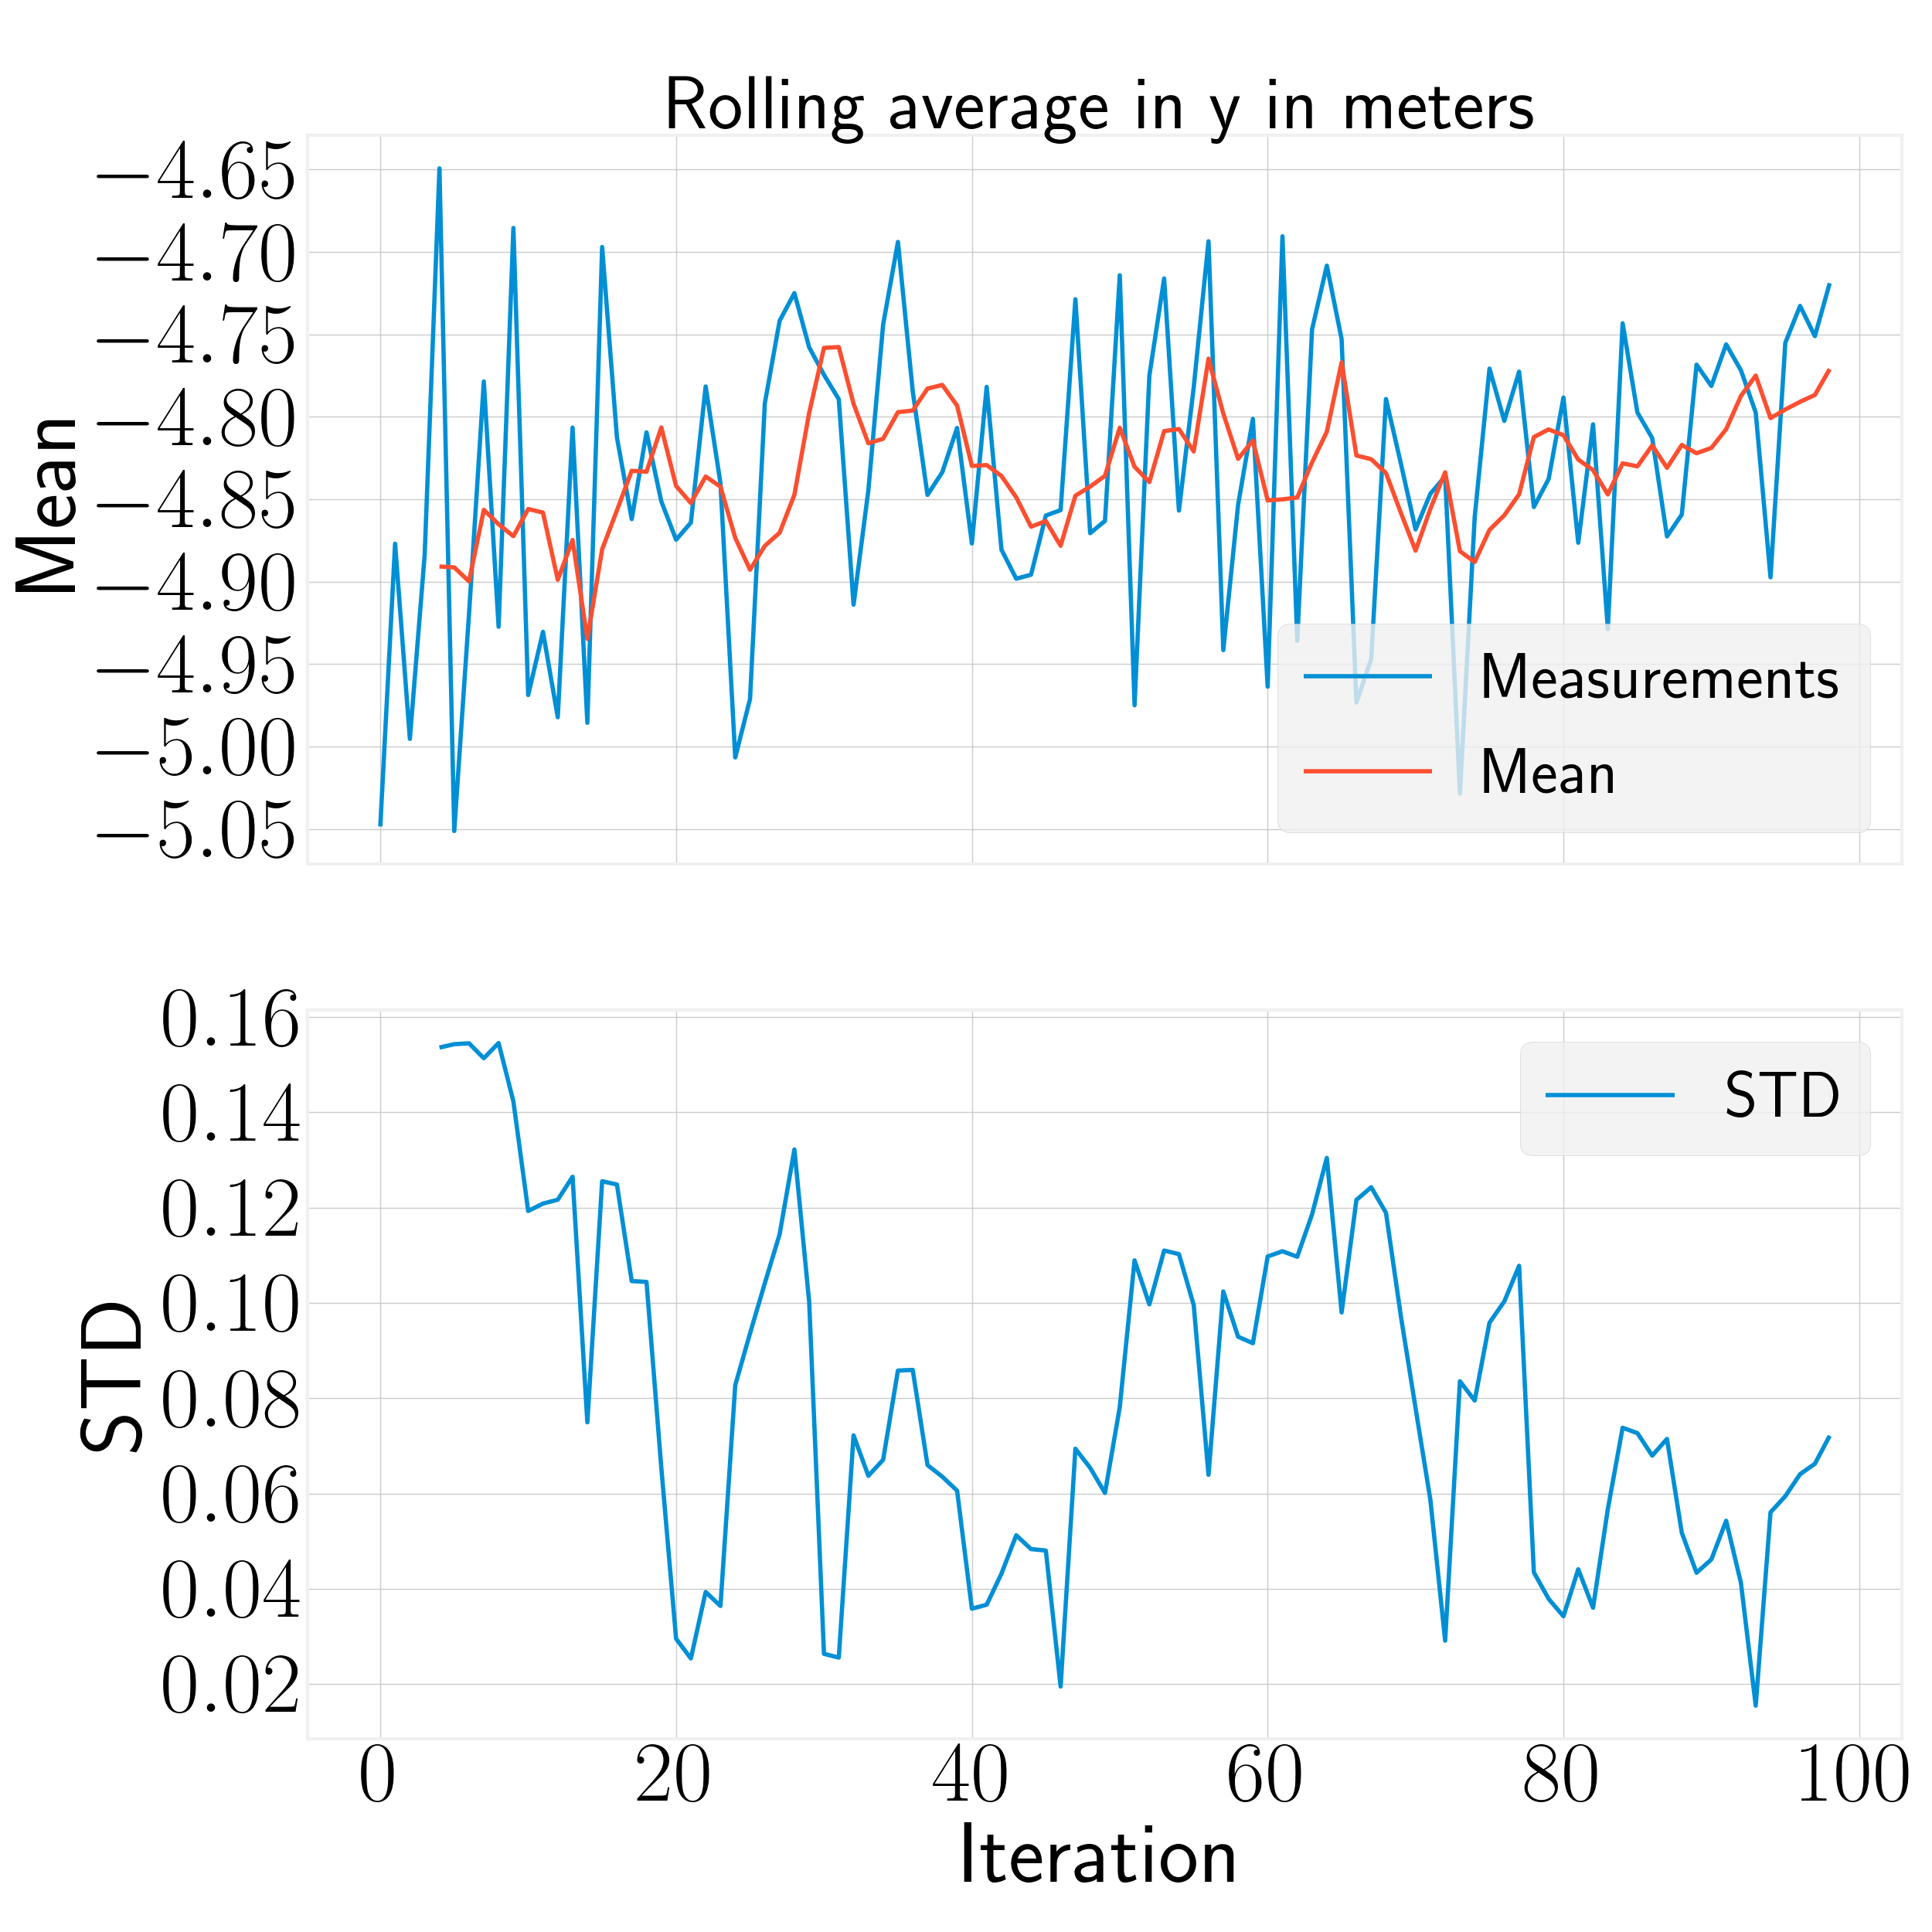
\includegraphics[width=\textwidth]{../Figures/analyse_rolling_average/test2/Calculated_rolling_average_in_y_with_mean_and_STD.png}
        \caption{}
        \label{fig:rolling_average_in_y_test2}
    \end{subfigure}
     \hspace{0.2em}
    \begin{subfigure}[t]{.30\textwidth}
        \centering
        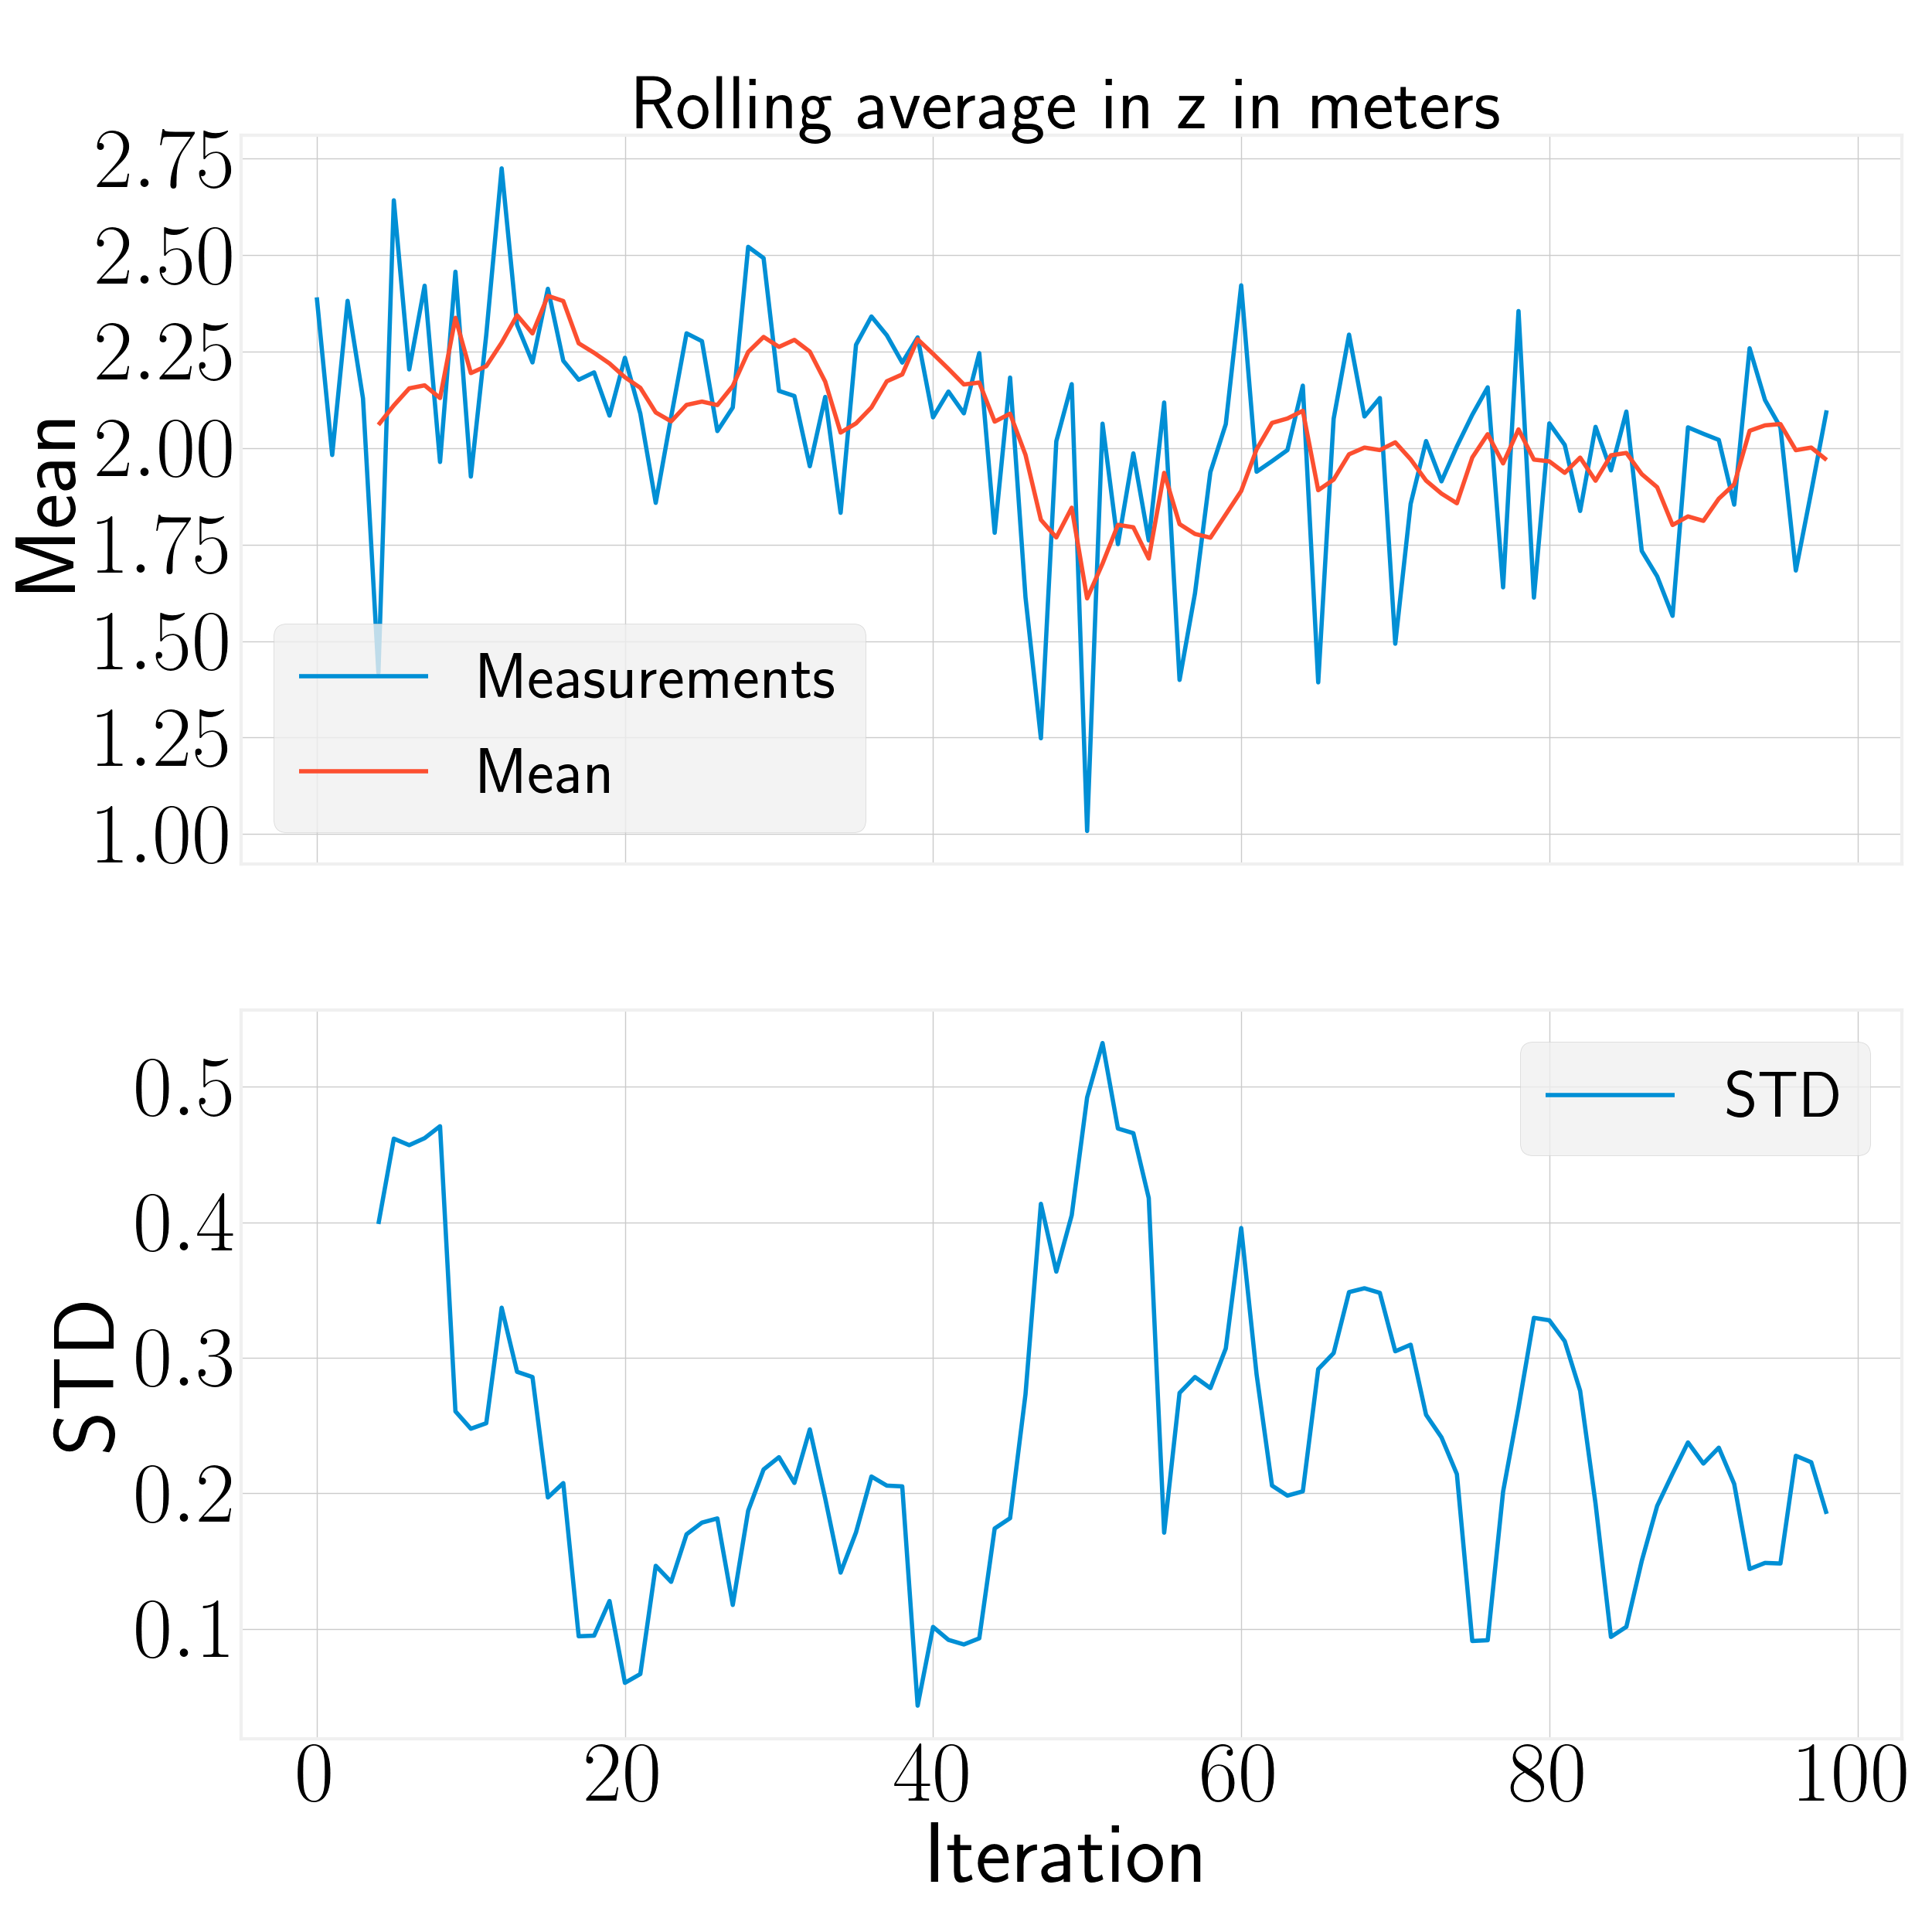
\includegraphics[width=\textwidth]{../Figures/analyse_rolling_average/test2/Calculated_rolling_average_in_z_with_mean_and_STD.png}
        \caption{}
        \label{fig:rolling_average_in_z_test2}
    \end{subfigure}
    \caption{}
    \label{fig:rolling_average_pos_test2}
\end{figure}

\begin{figure}[H]
    \centering
    \begin{subfigure}[t]{.30\textwidth}
        \centering
        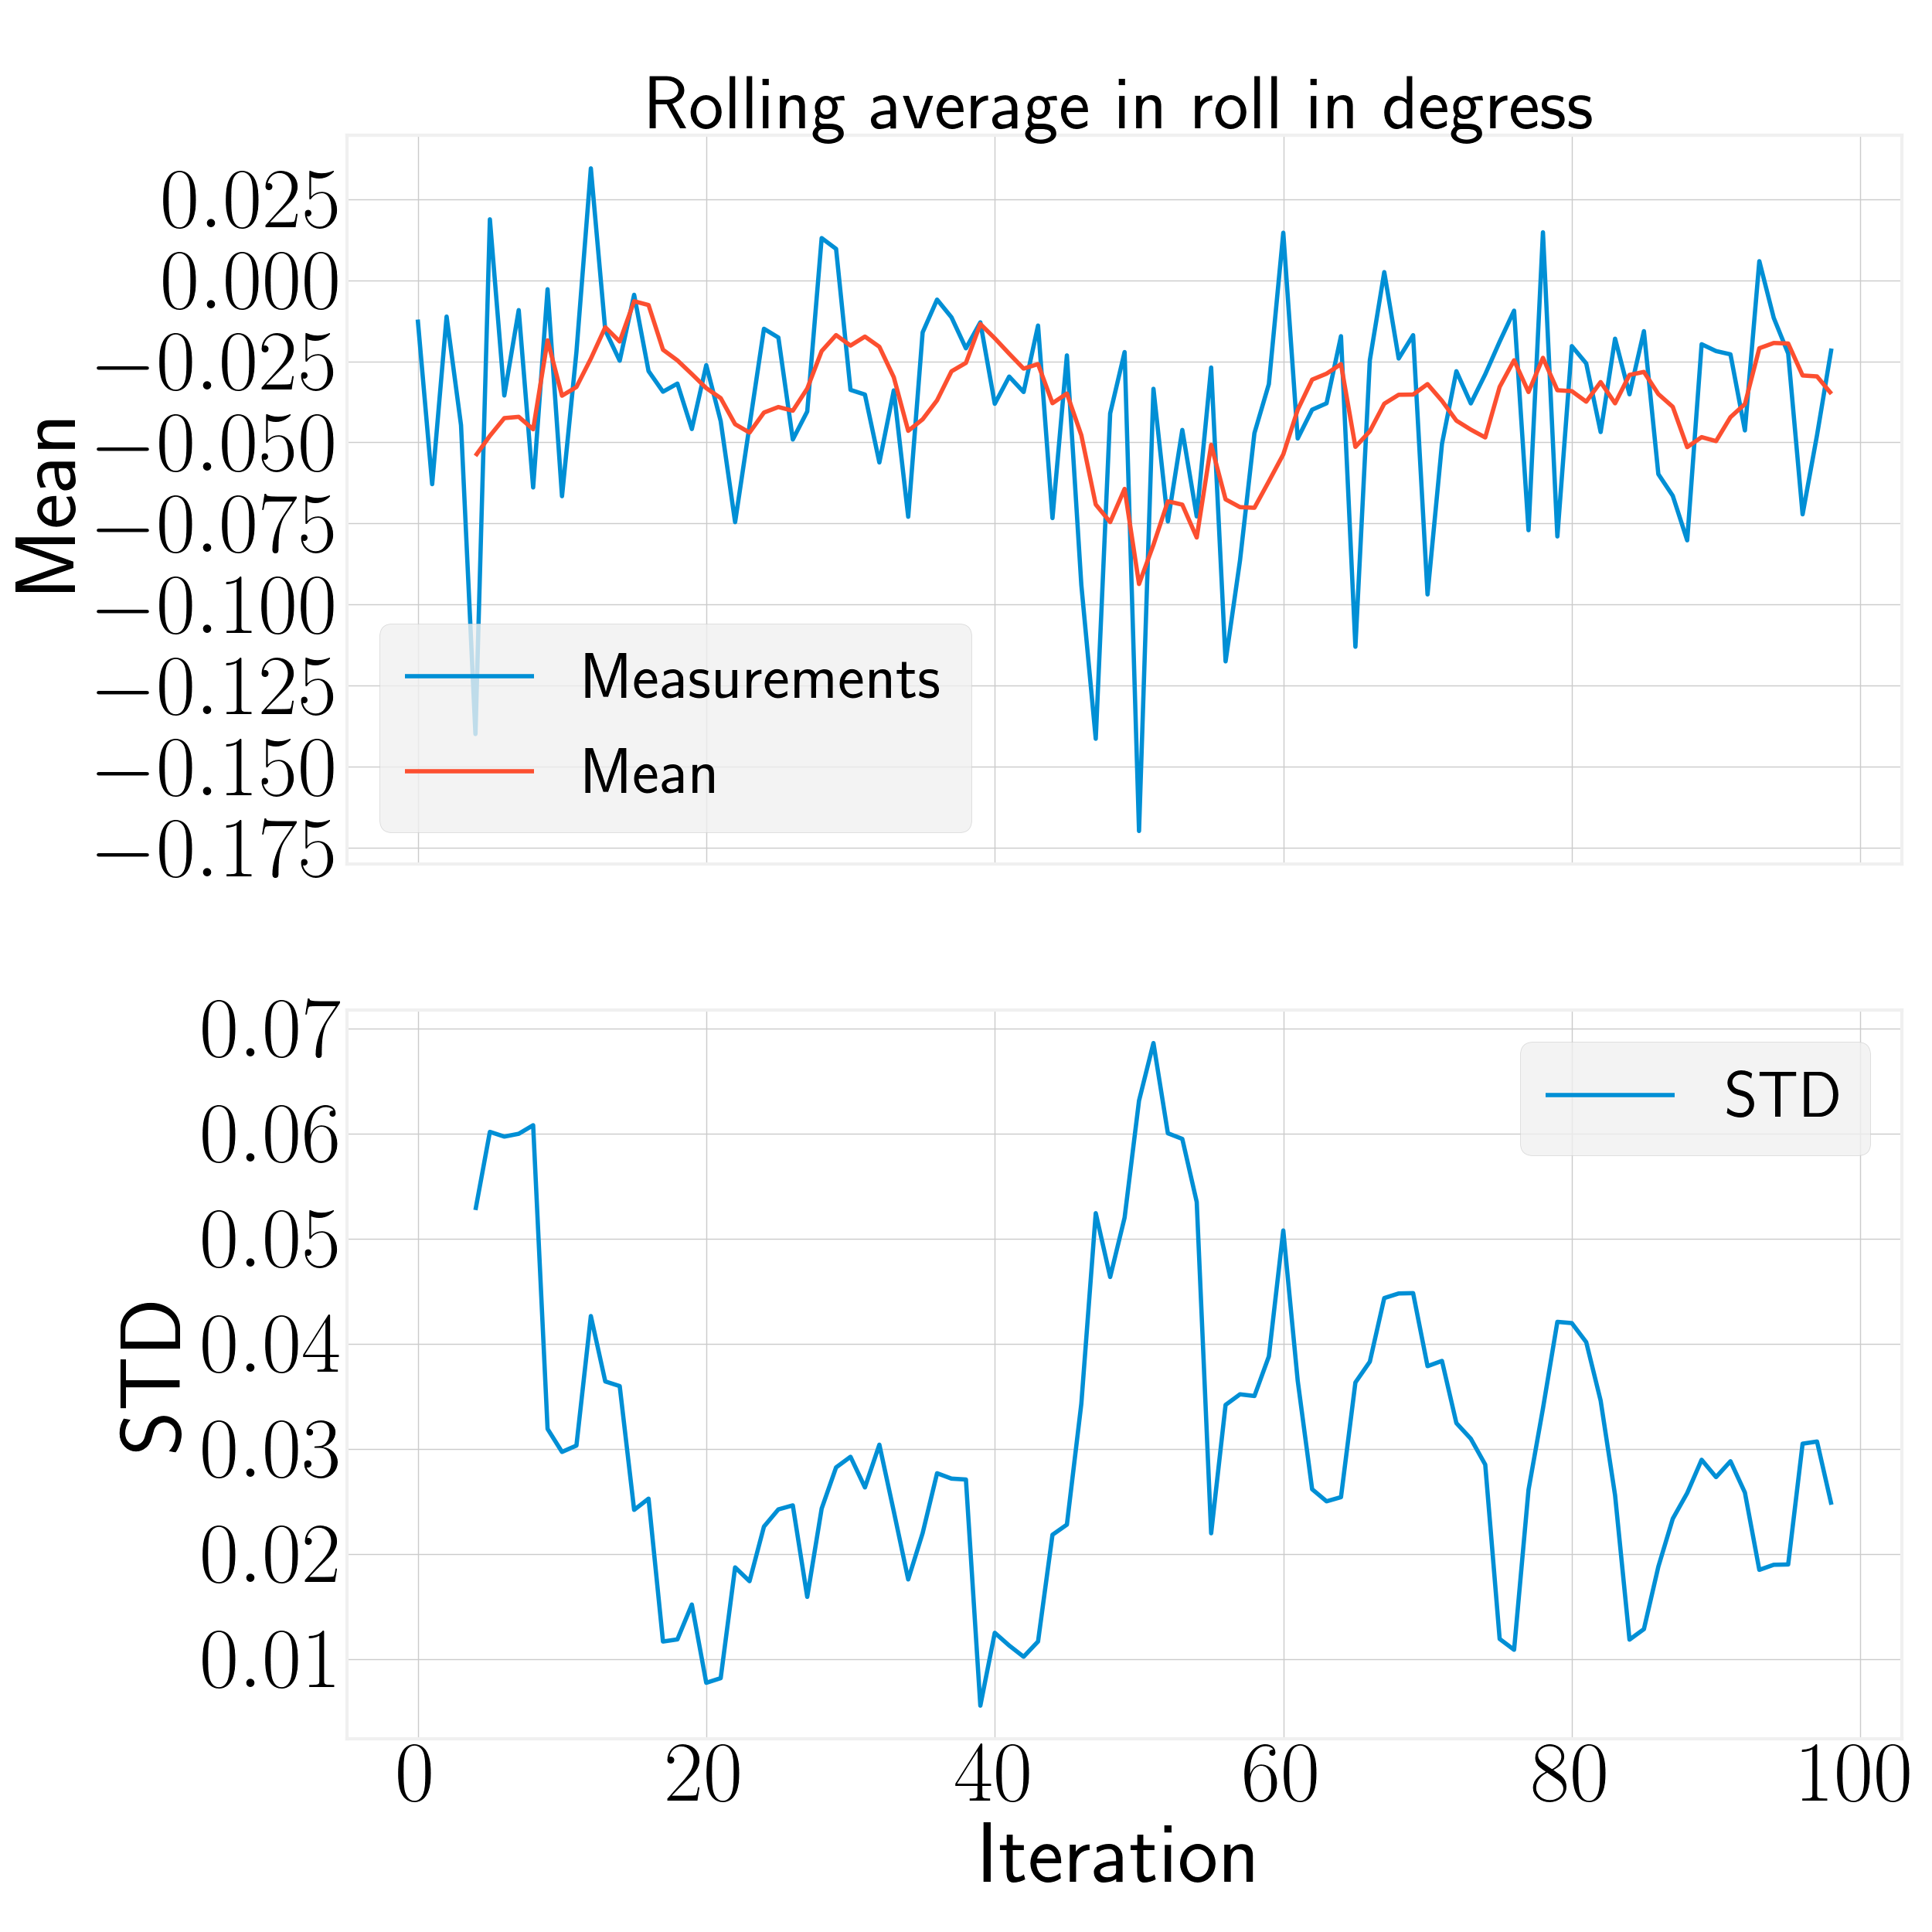
\includegraphics[width=\textwidth]{../Figures/analyse_rolling_average/test2/Calculated_rolling_average_in_roll_with_mean_and_STD.png}
        \caption{}
        \label{fig:rolling_average_in_roll_test2}
    \end{subfigure}
     \hspace{0.2em}
    \begin{subfigure}[t]{.30\textwidth}
        \centering
        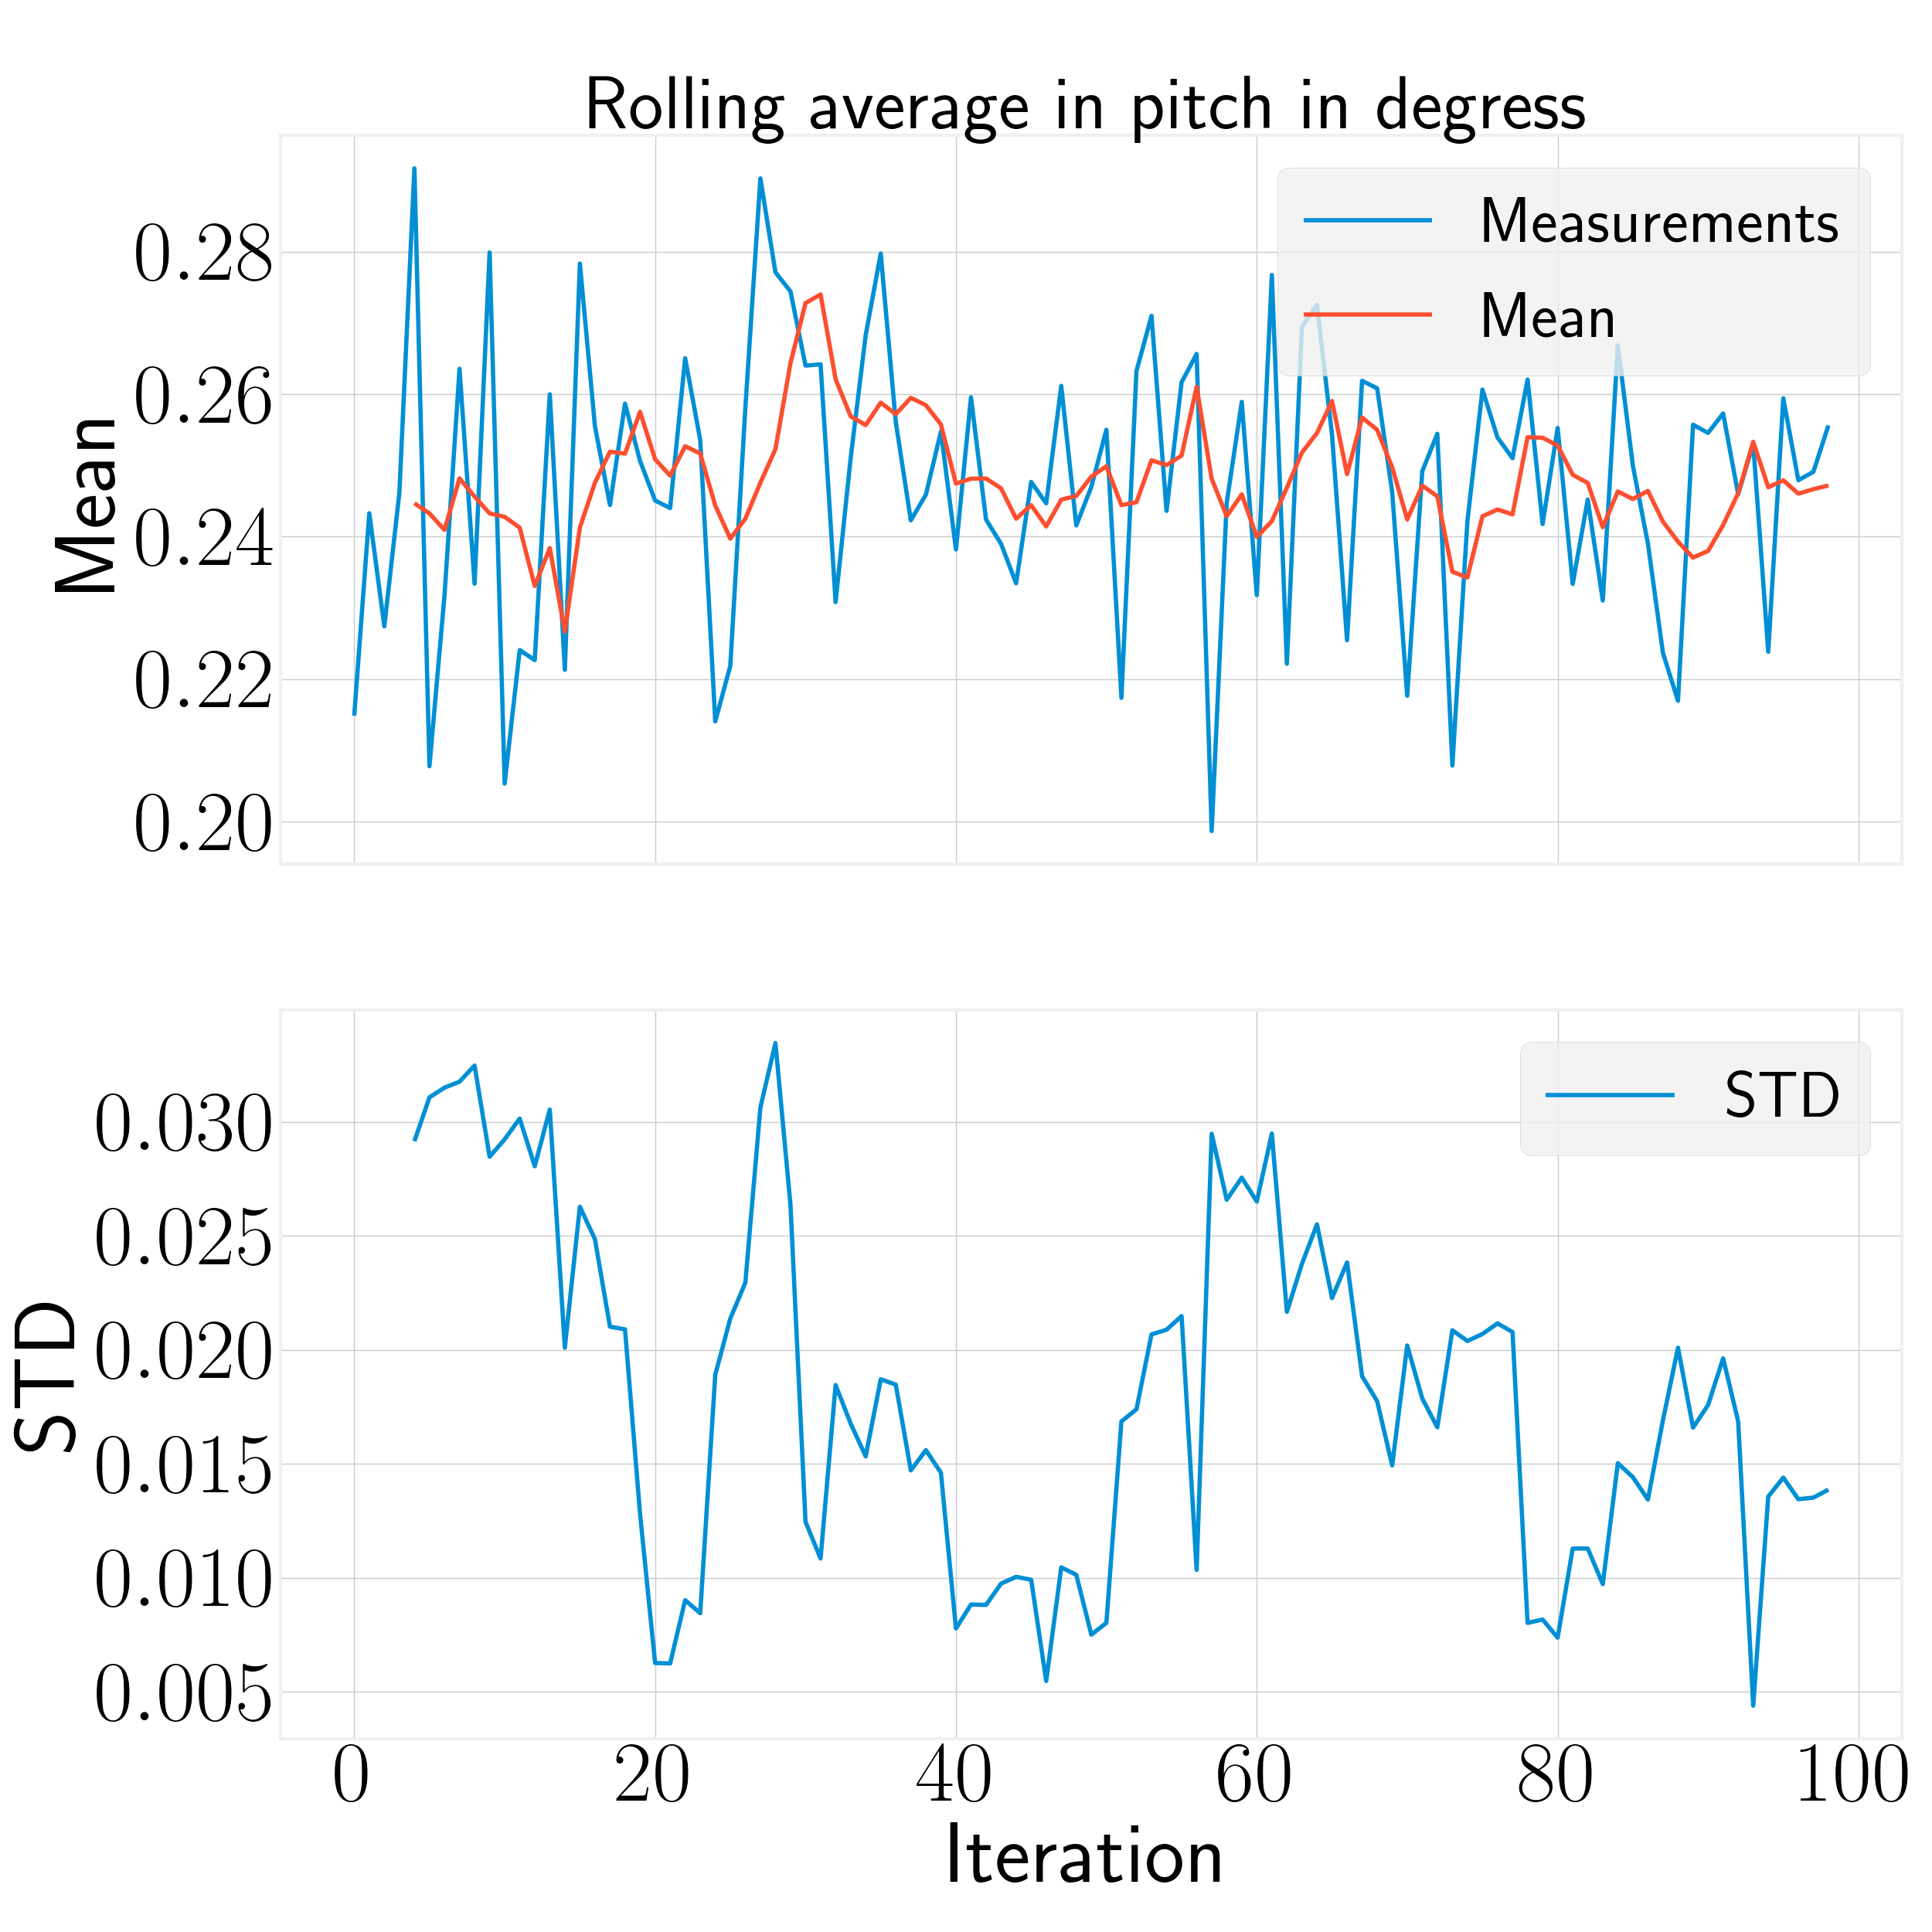
\includegraphics[width=\textwidth]{../Figures/analyse_rolling_average/test2/Calculated_rolling_average_in_pitch_with_mean_and_STD.png}
        \caption{}
        \label{fig:rolling_average_in_pitch_test2}
    \end{subfigure}
     \hspace{0.2em}
    \begin{subfigure}[t]{.30\textwidth}
        \centering
        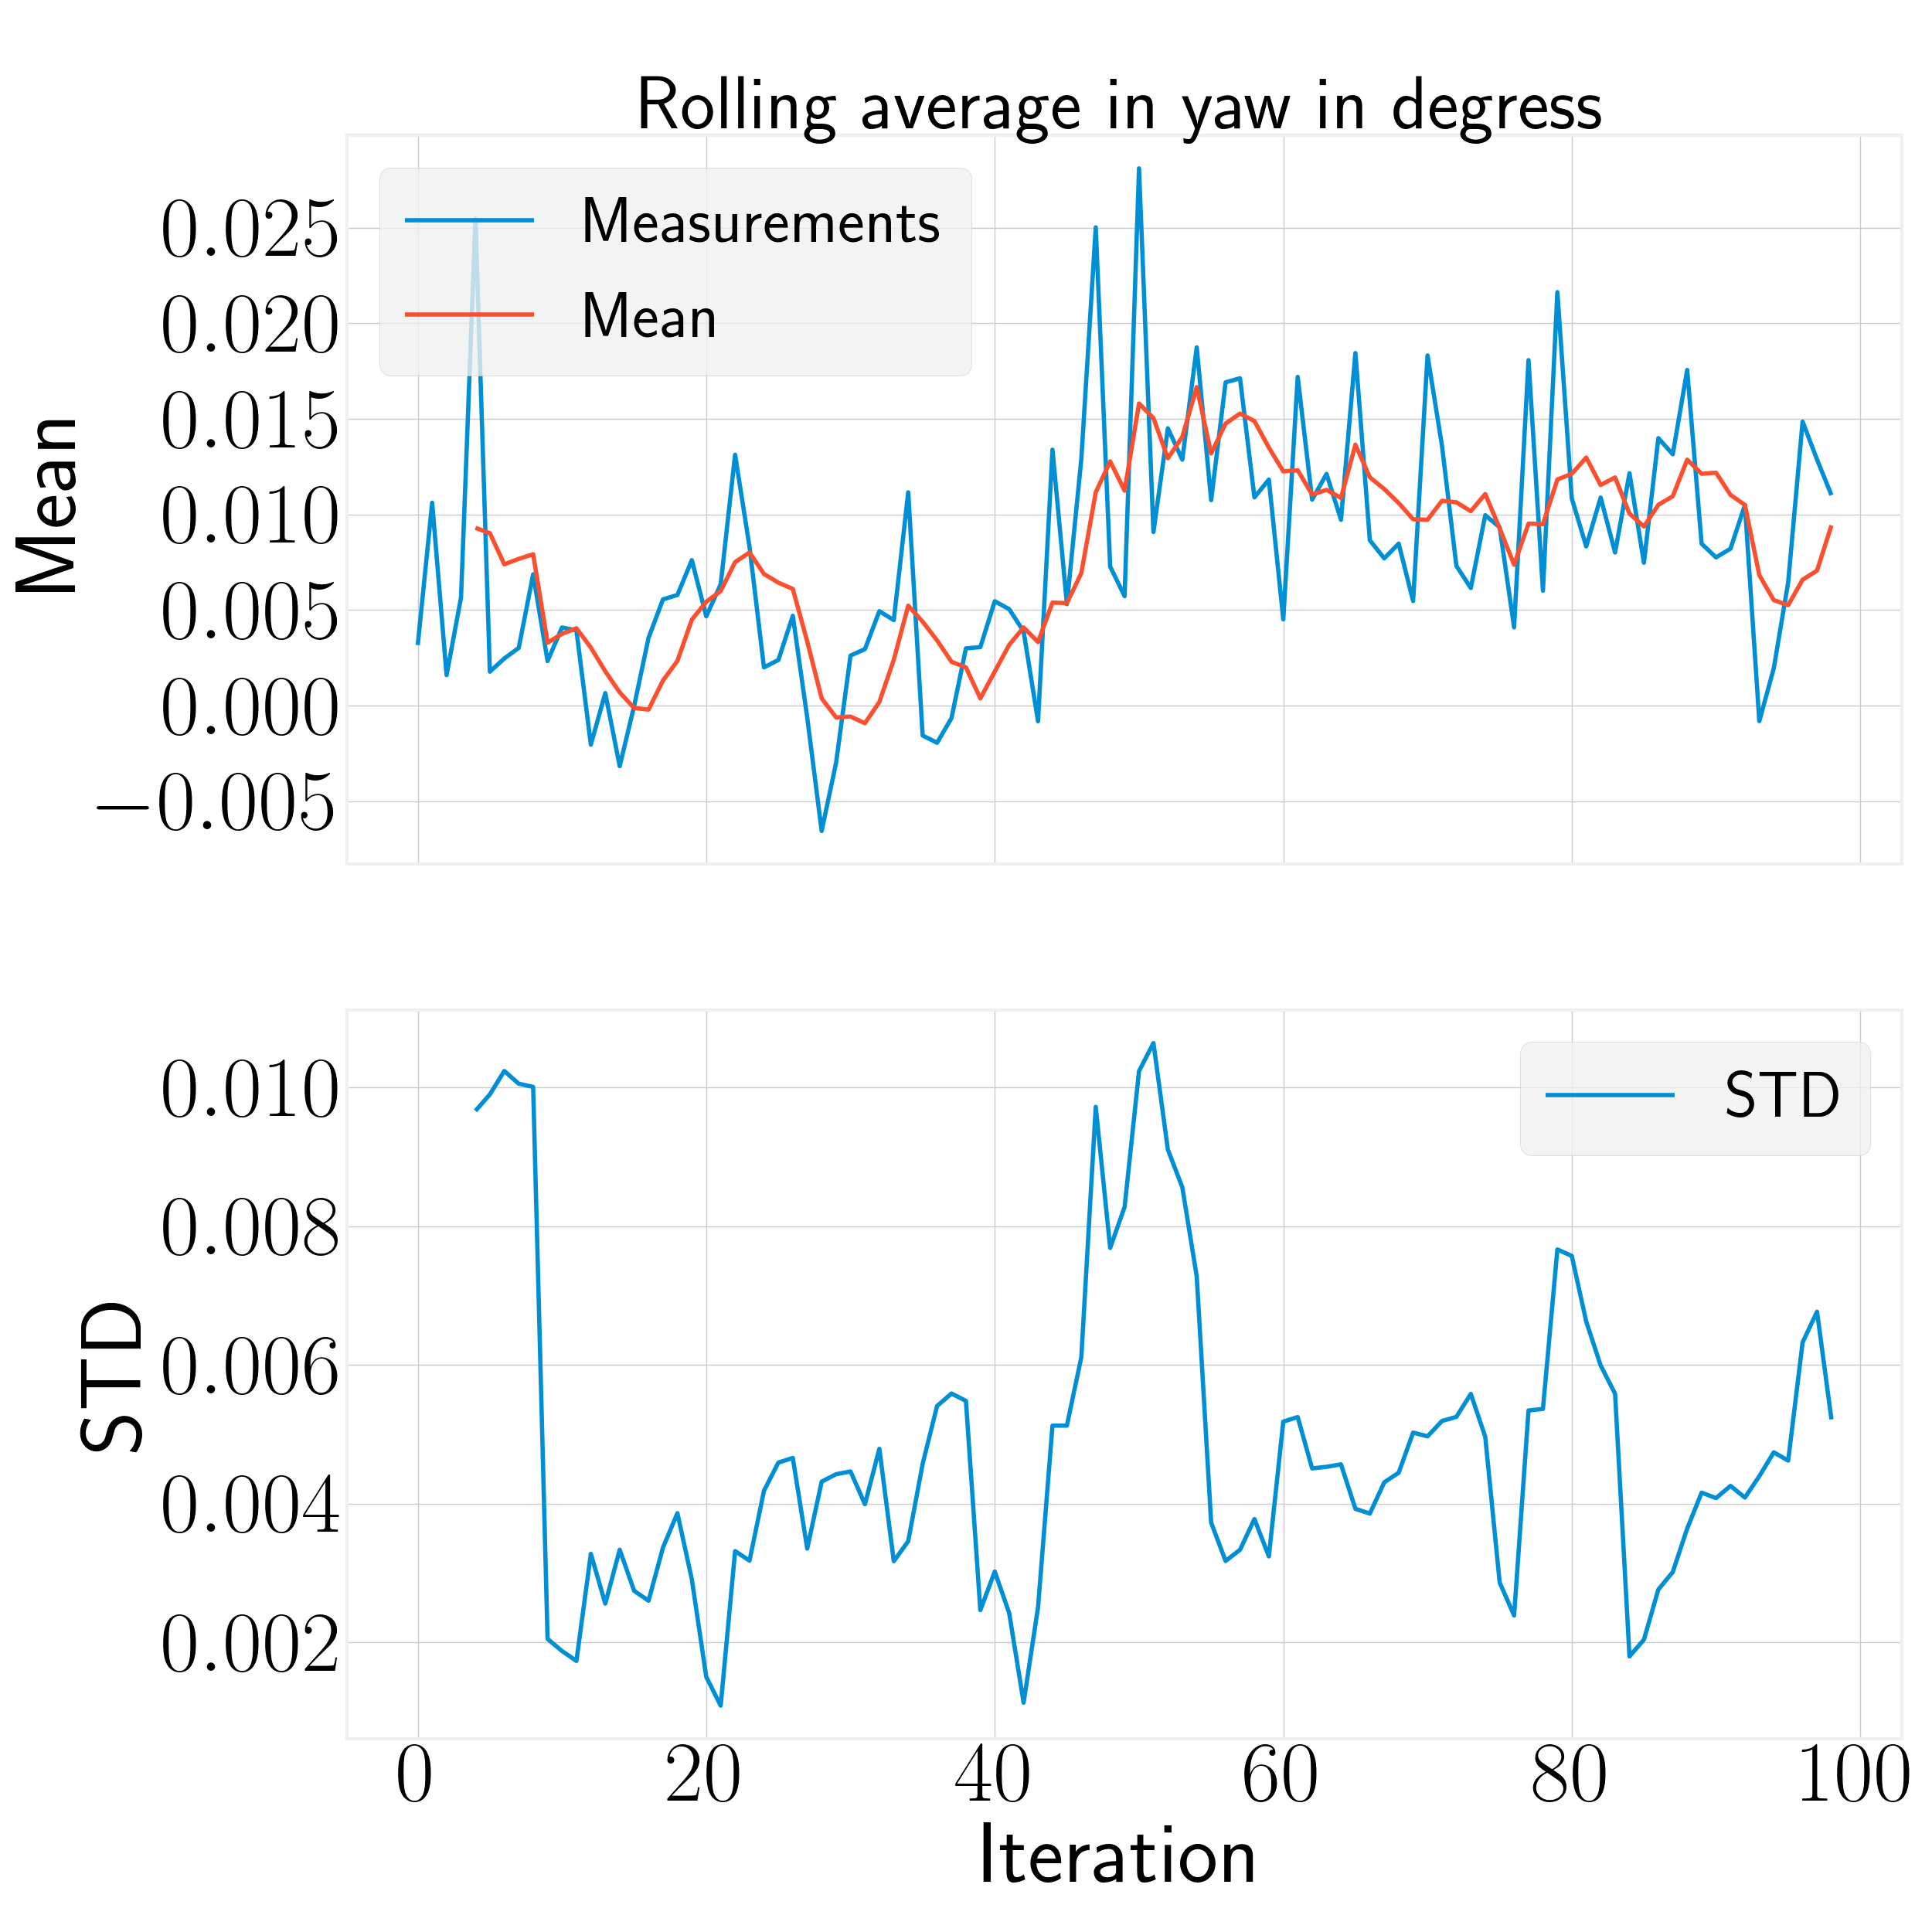
\includegraphics[width=\textwidth]{../Figures/analyse_rolling_average/test2/Calculated_rolling_average_in_yaw_with_mean_and_STD.png}
        \caption{}
        \label{fig:rolling_average_in_yaw_test2}
    \end{subfigure}
    \caption{}
    \label{fig:rolling_average_angle_test2}
\end{figure}


\subsubsection{Hold pose using ArUco pose estimation}

\begin{figure}[H]
    \centering
    \begin{subfigure}[t]{.30\textwidth}
        \centering
        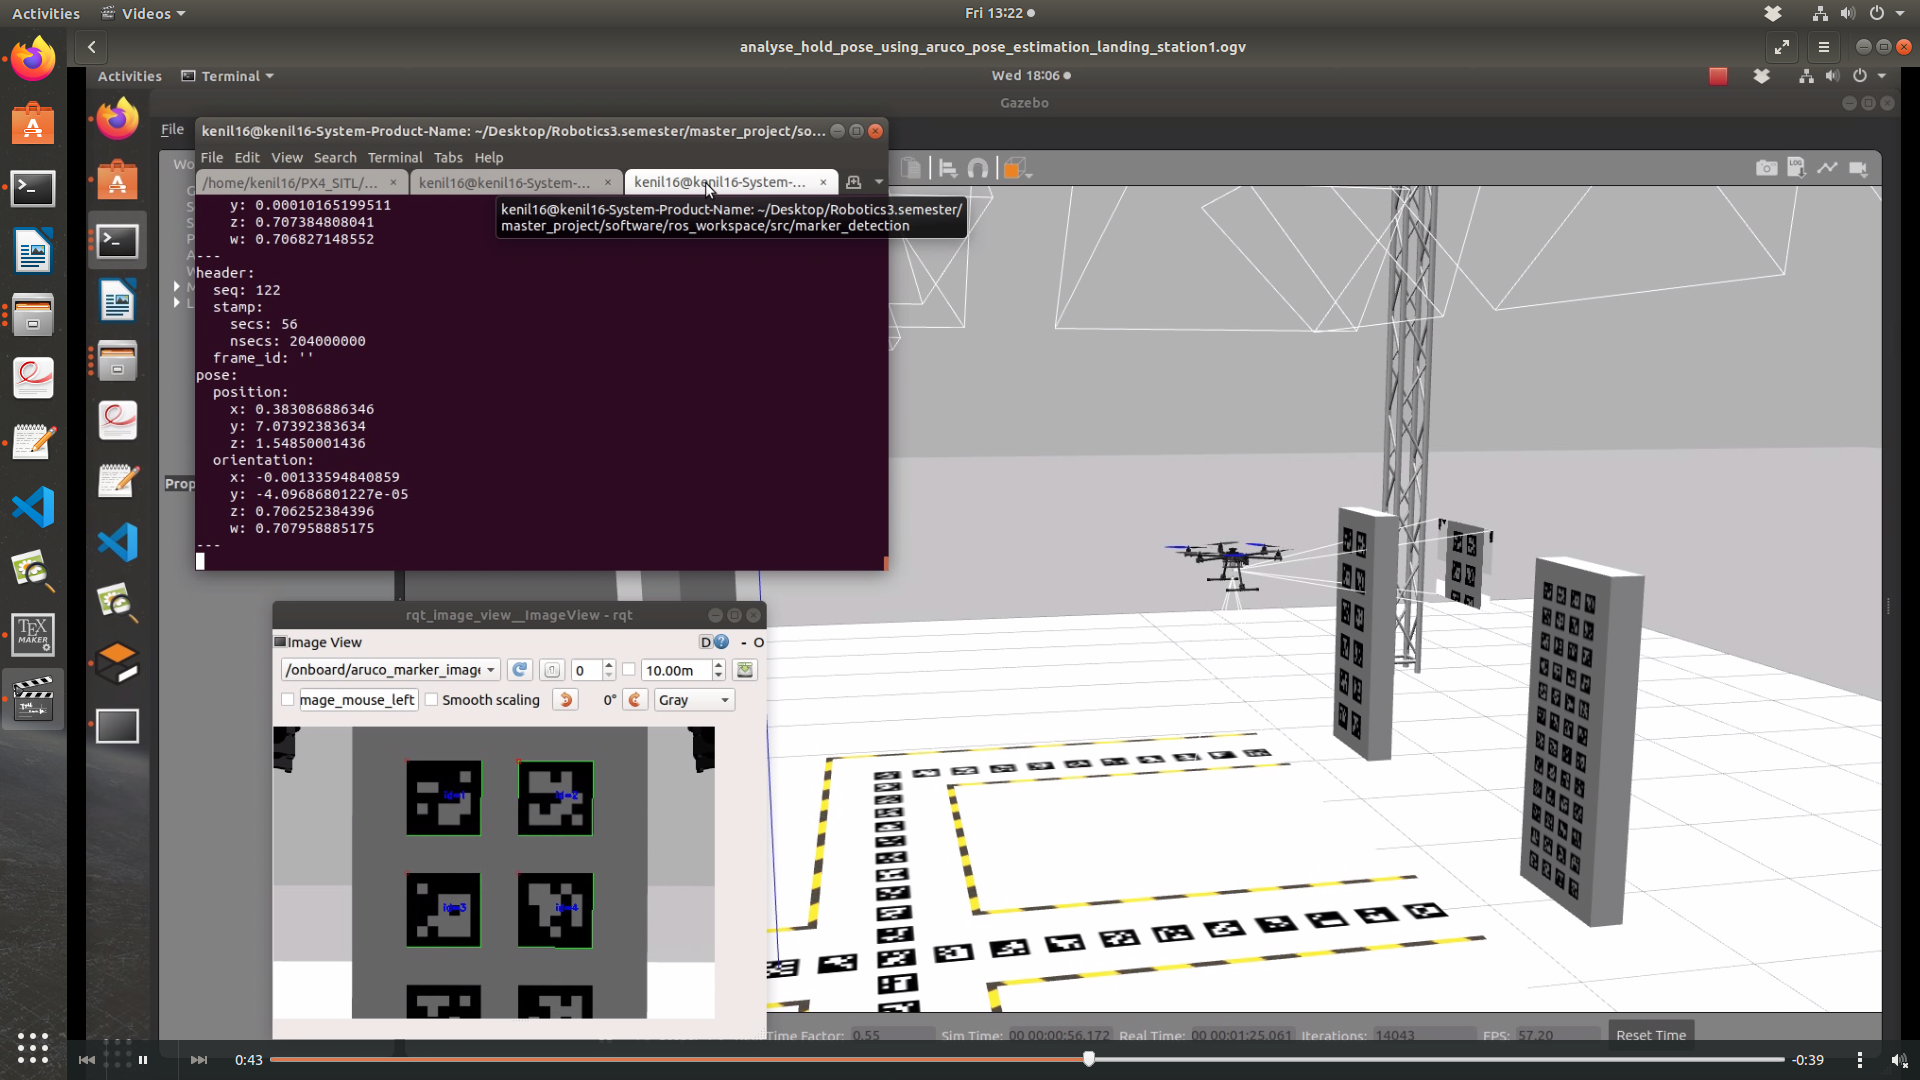
\includegraphics[width=\textwidth]{../Figures/hold_pose_using_aruco_pose_estimation/aruco_board_three.png}
        \caption{}
        \label{fig:hold_pose_aruco_board_three}
    \end{subfigure}
     \hspace{0.2em}
    \begin{subfigure}[t]{.30\textwidth}
        \centering
        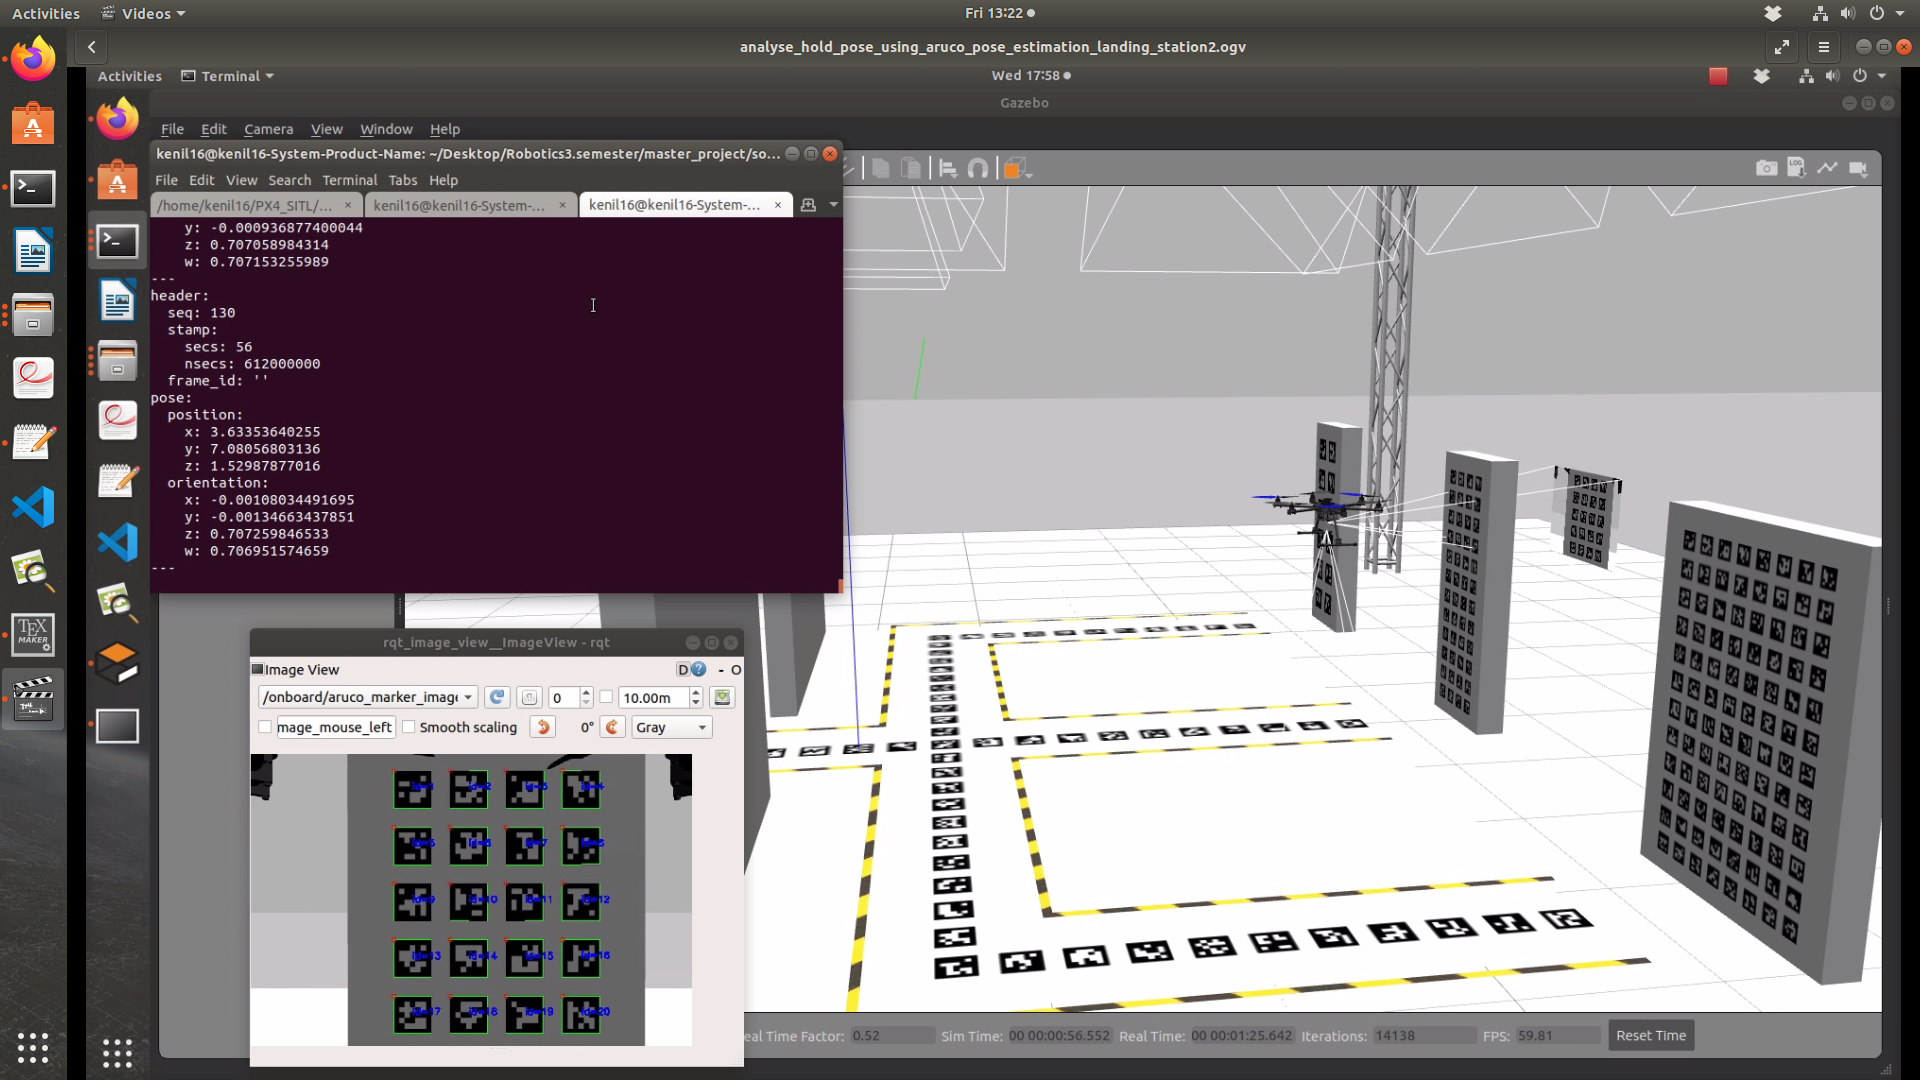
\includegraphics[width=\textwidth]{../Figures/hold_pose_using_aruco_pose_estimation/aruco_board_four.png}
        \caption{}
        \label{fig:hold_pose_aruco_board_four}
    \end{subfigure}
     \hspace{0.2em}
    \begin{subfigure}[t]{.30\textwidth}
        \centering
        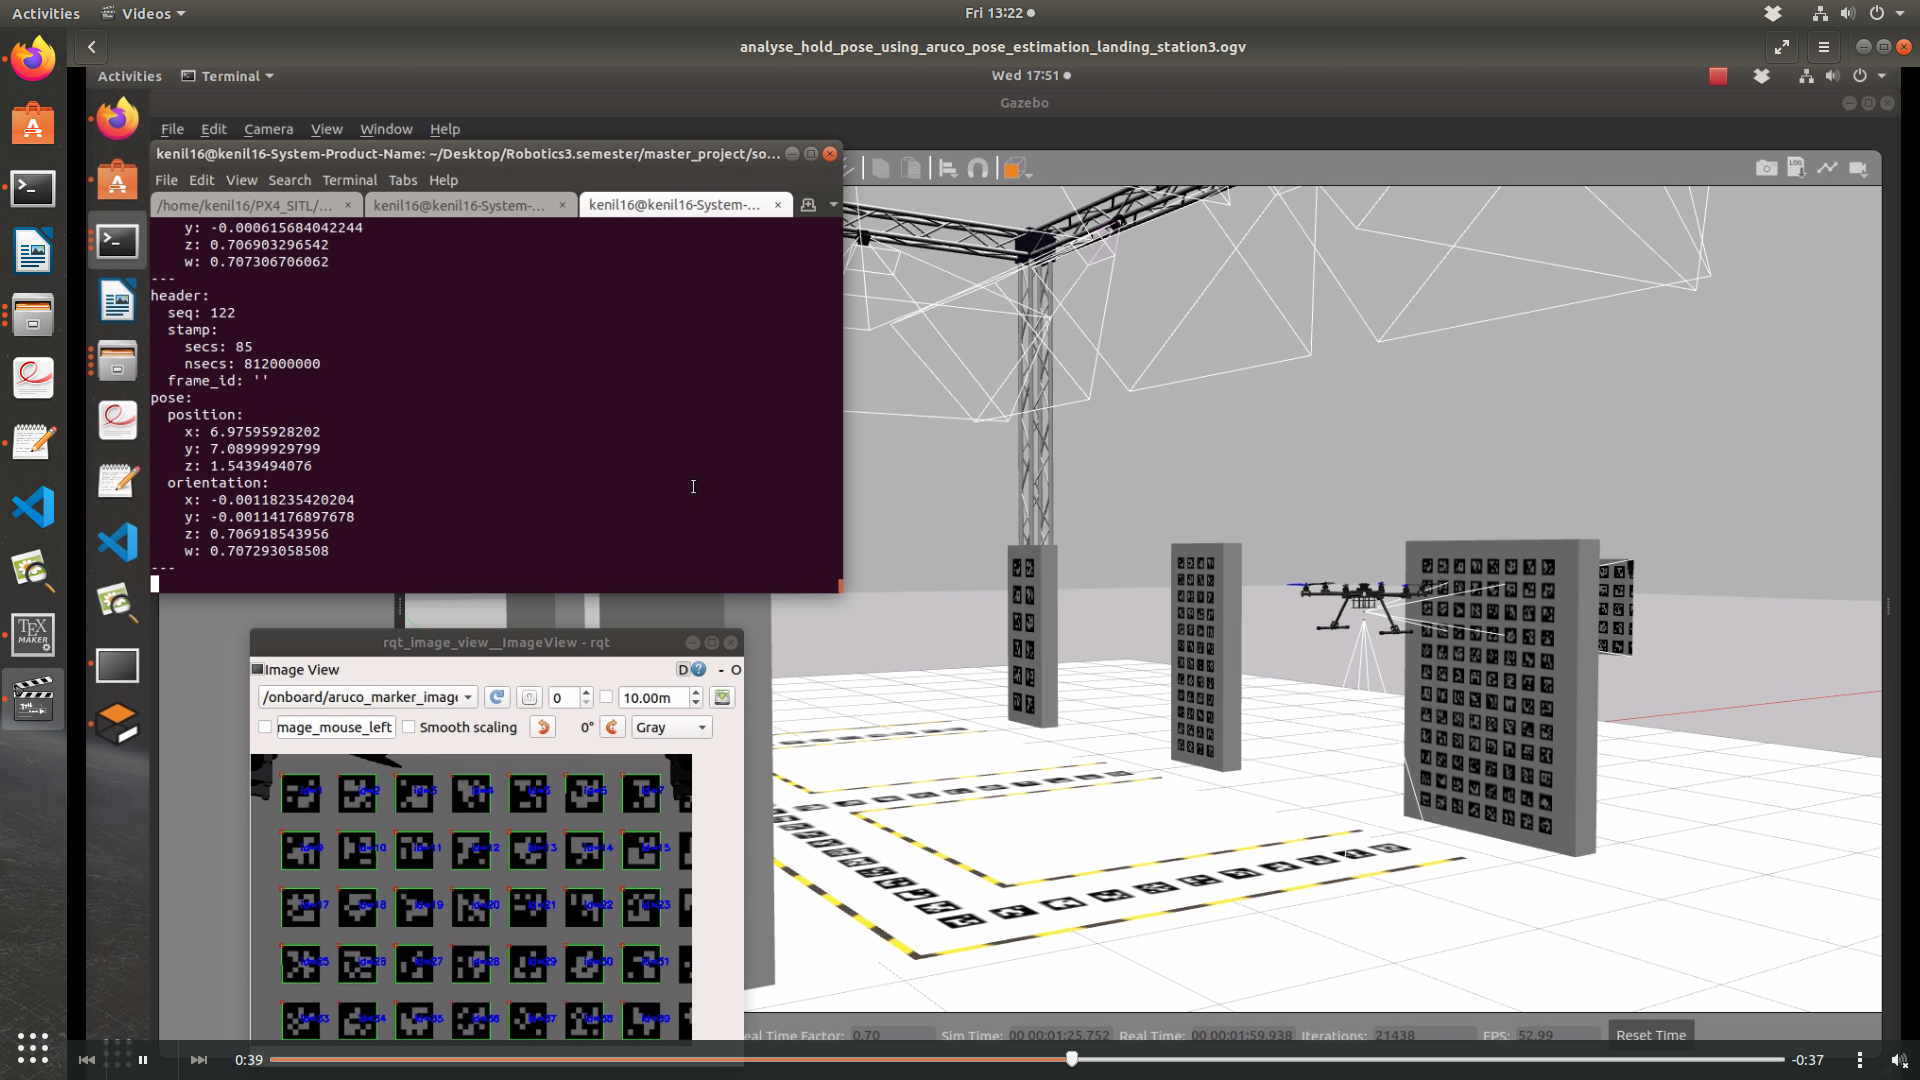
\includegraphics[width=\textwidth]{../Figures/hold_pose_using_aruco_pose_estimation/aruco_board_five.png}
        \caption{}
        \label{fig:hold_pose_aruco_board_five}
    \end{subfigure}
        \begin{subfigure}[t]{.30\textwidth}
        \centering
        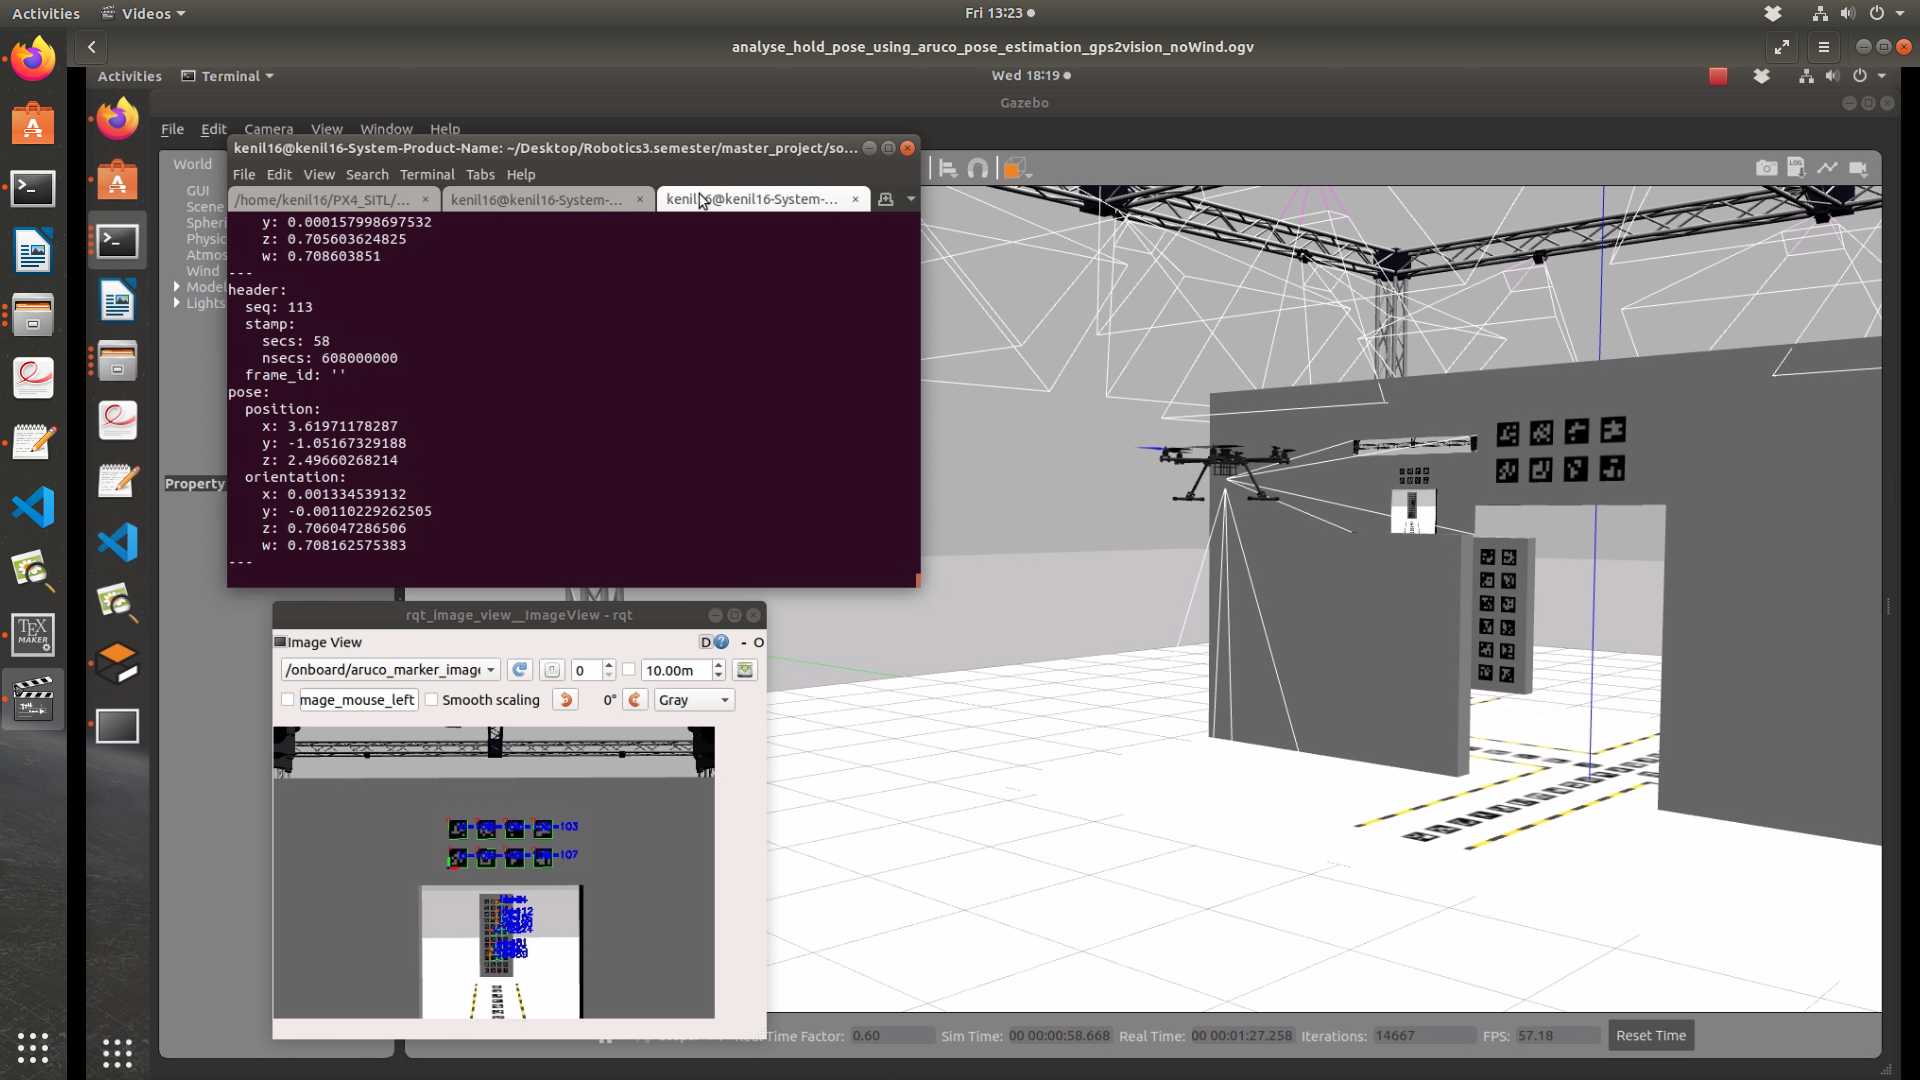
\includegraphics[width=\textwidth]{../Figures/hold_pose_using_aruco_pose_estimation/aruco_board_one_noWind.png}
        \caption{}
        \label{fig:hold_pose_aruco_board_one_noWind}
    \end{subfigure}
        \begin{subfigure}[t]{.30\textwidth}
        \centering
        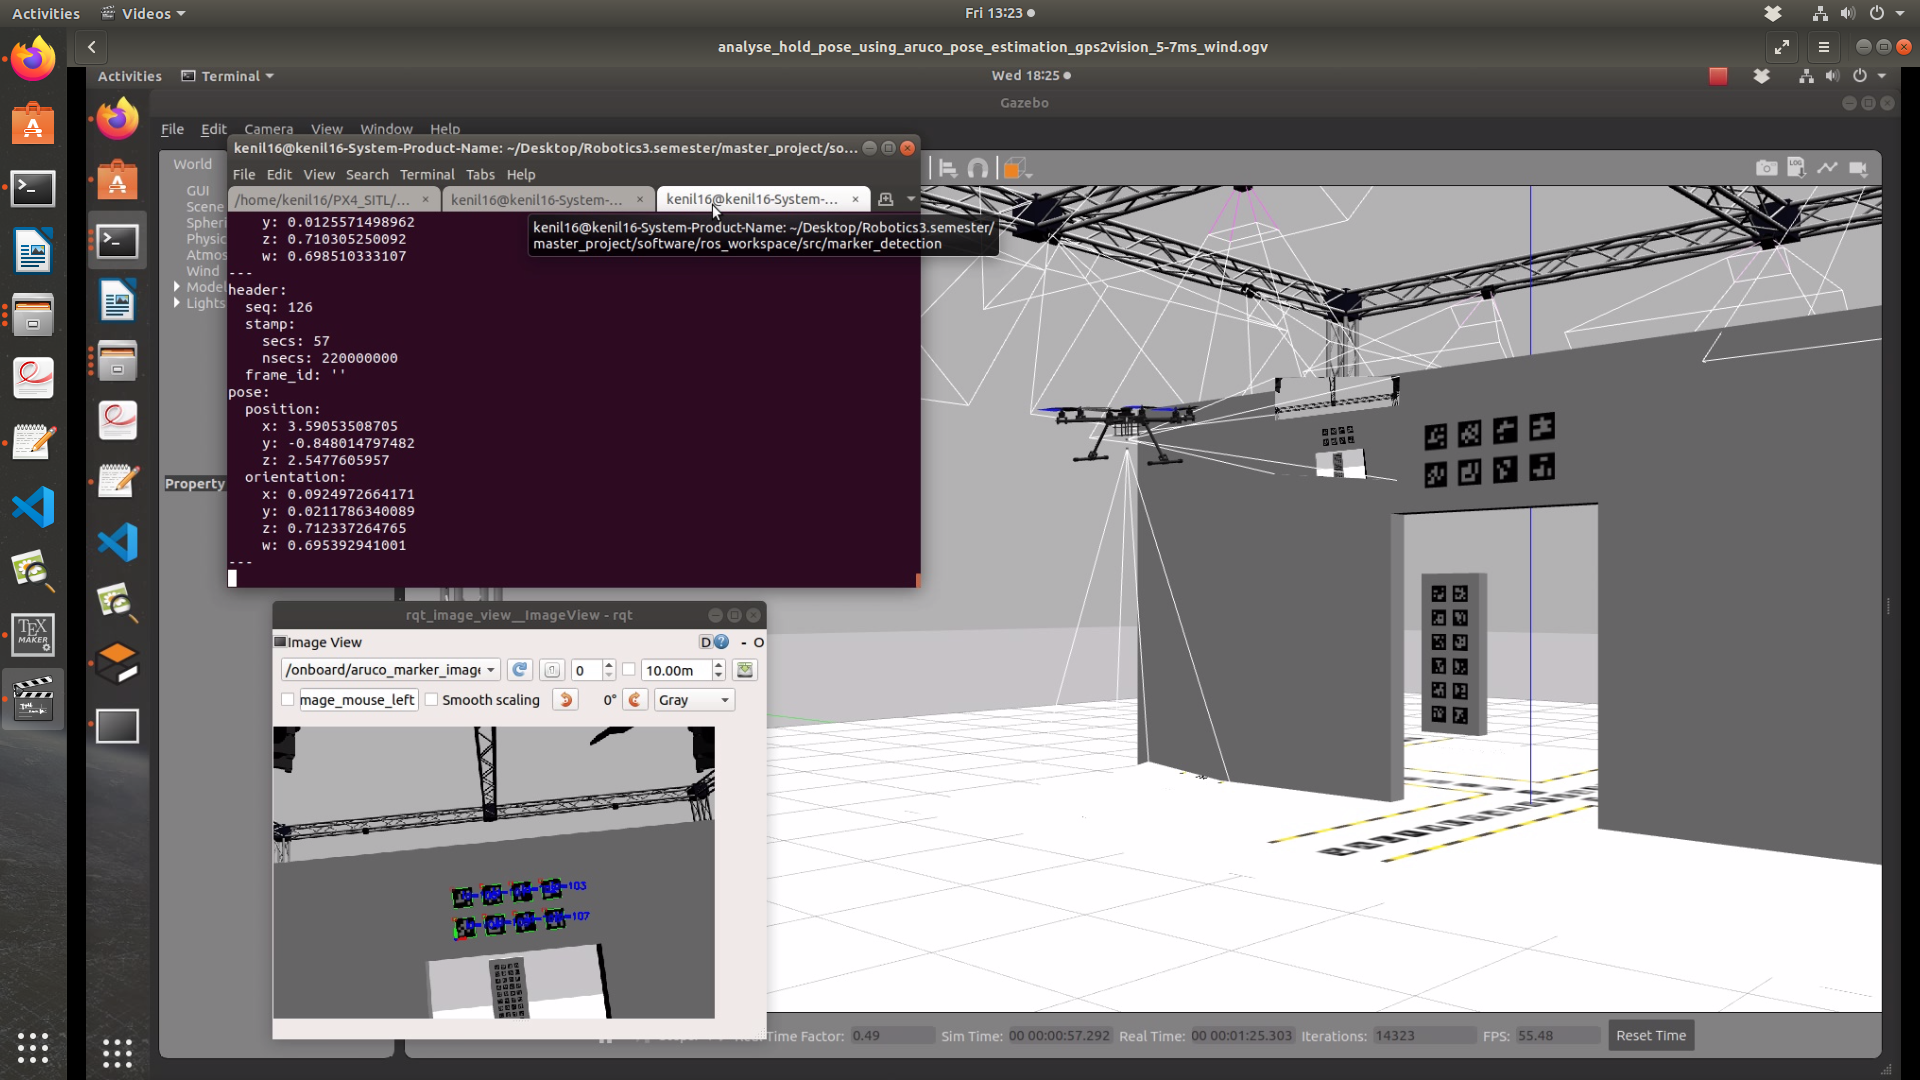
\includegraphics[width=\textwidth]{../Figures/hold_pose_using_aruco_pose_estimation/aruco_board_one_5-7ms_wind.png}
        \caption{}
        \label{fig:hold_pose_aruco_board_one_5-7ms_wind}
    \end{subfigure}
    \caption{}
    \label{fig:hold_pose_aruco_boards}
\end{figure}

\begin{table}[H]
    \centering
    \addtolength{\leftskip} {-2cm}
    \addtolength{\rightskip}{-2cm}
        \caption{Statistics of the results from landing tests }
        \pgfplotstabletypeset[normal,
                columns/eg/.style={
                column name={Runs},
                dec sep align
        }
        ]{ %
        Estimation error & eg & Wind & Mean position & STD position & Mean angle & STD angle\\
        \topmidheader{8}{\textbf{Test 1}}
ArUco pose         & 10      & No & $1.43cm$ & $1.10cm$ & $0.18^{\circ}$ & $0.13^{\circ}$\\
Setpoint         & 10      & No & $3.12cm $ & $2.58cm$ & $0.28^{\circ}$ & $0.22^{\circ}$\\
		\midheader{8}{\textbf{Test 2}}
ArUco pose         & 10      & Yes & $1.47cm $ & $0.95cm$ & $0.49^{\circ}$ & $0.31^{\circ}$\\
Setpoint         & 10      & Yes & $4.04cm $ & $3.35cm$ & $4.45^{\circ}$ & $1.49^{\circ}$\\
 }
\end{table}

\begin{table}[H]
    \centering
    \addtolength{\leftskip} {-2cm}
    \addtolength{\rightskip}{-2cm}
        \caption{Statistics of the results from landing tests }
        \pgfplotstabletypeset[normal,
                columns/eg/.style={
                column name={Runs},
                dec sep align
        }
        ]{ %
        Estimation error & eg & Wind & Mean position & STD position & Mean angle & STD angle\\
        \topmidheader{8}{\textbf{Test 3}}
ArUco pose         & 10      & No & $0.12cm $ & $0.23cm$ & $0.03^{\circ}$ & $0.05^{\circ}$\\
Setpoint         & 10      & No & $2.93cm$ & $2.90cm$ & $0.12^{\circ}$ & $0.12^{\circ}$\\
		\midheader{8}{\textbf{Test 4}}
ArUco pose         & 10      & No & $0.11cm $ & $0.21cm$ & $0.02^{\circ}$ & $0.01^{\circ}$\\
Setpoint         & 10      & No & $2.92cm$ & $2.89cm$ & $0.11^{\circ}$ & $0.09^{\circ}$\\
		\midheader{8}{\textbf{Test 5}}
ArUco pose         & 10      & No & $0.09cm $ & $0.20cm$ &
$0.02^{\circ}$ & $0.01^{\circ}$\\
Setpoint         & 10      & No & $2.89cm$ & $2.85cm$ & $0.11^{\circ}$ & $0.09^{\circ}$\\
 }
\end{table}


\begin{figure}[H]
    \centering
    \begin{subfigure}[t]{.30\textwidth}
        \centering
        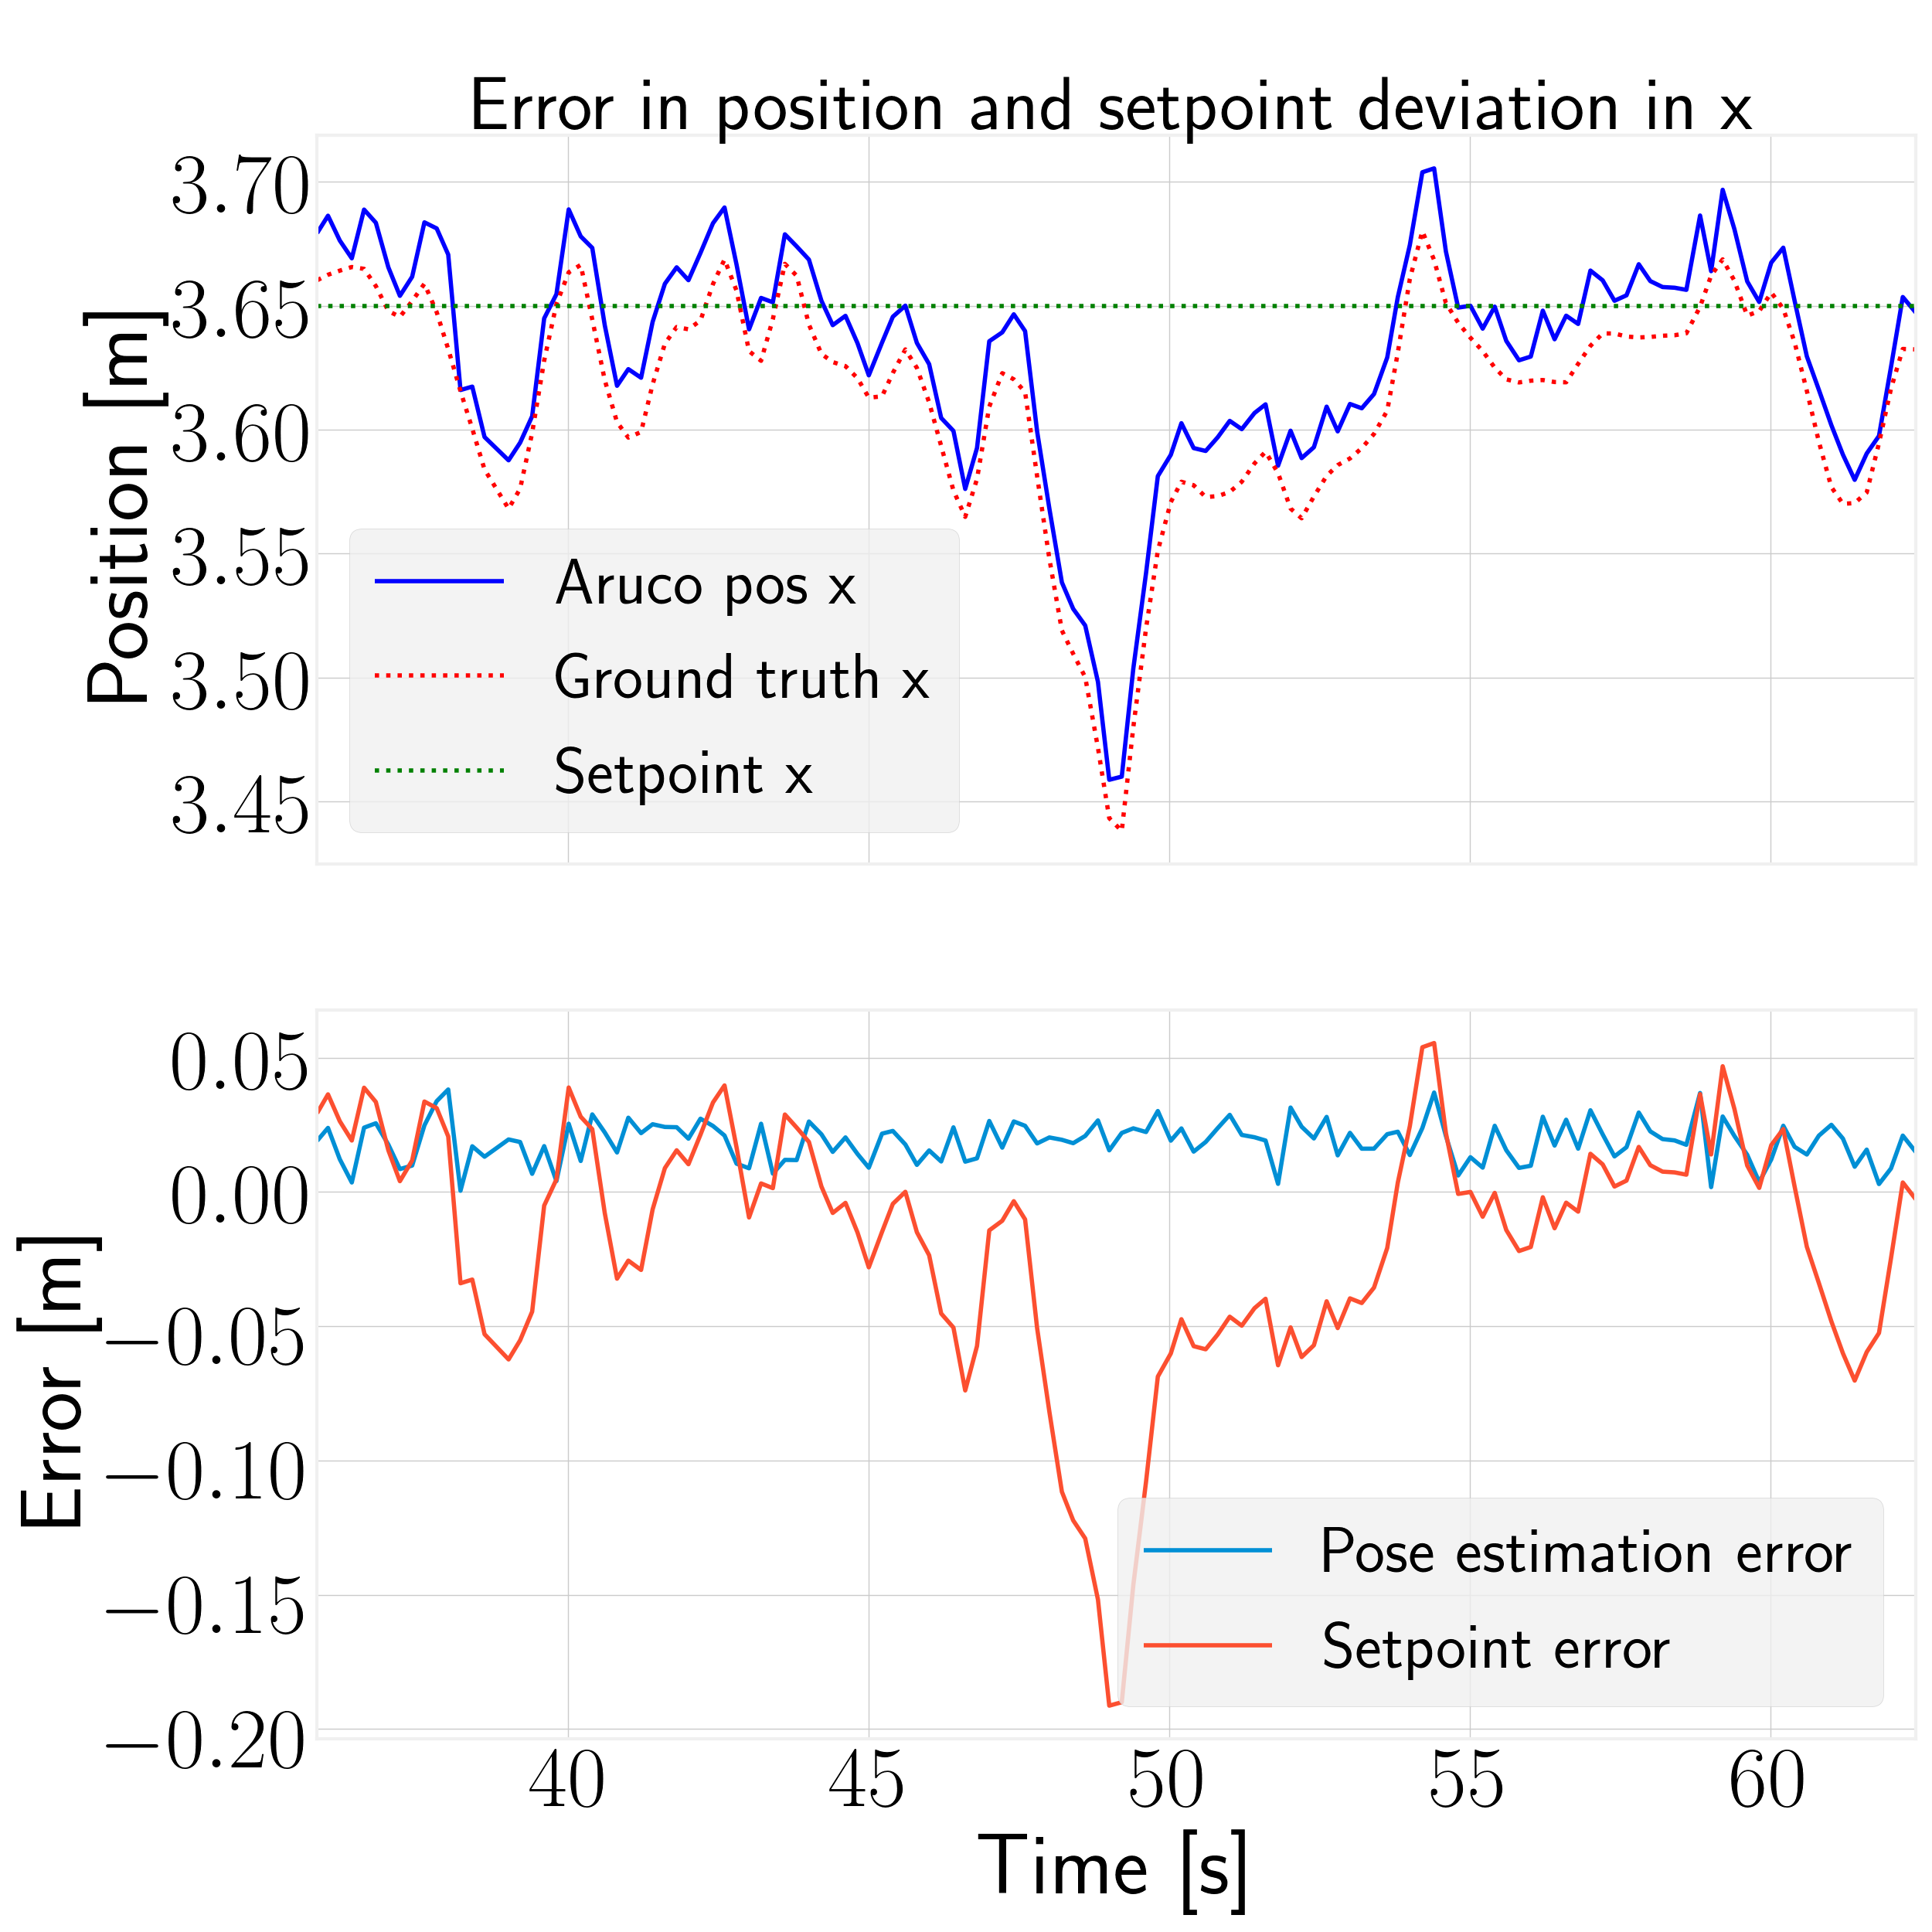
\includegraphics[width=\textwidth]{../Figures/hold_pose_using_aruco_pose_estimation/test2_gps2visionBoard_1.0Wind_-1.0y/error_x/pose_error_x_test1.png}
        \caption{}
        \label{fig:hold_pose_estimation_test2_x}
    \end{subfigure}
     \hspace{0.2em}
    \begin{subfigure}[t]{.30\textwidth}
        \centering
        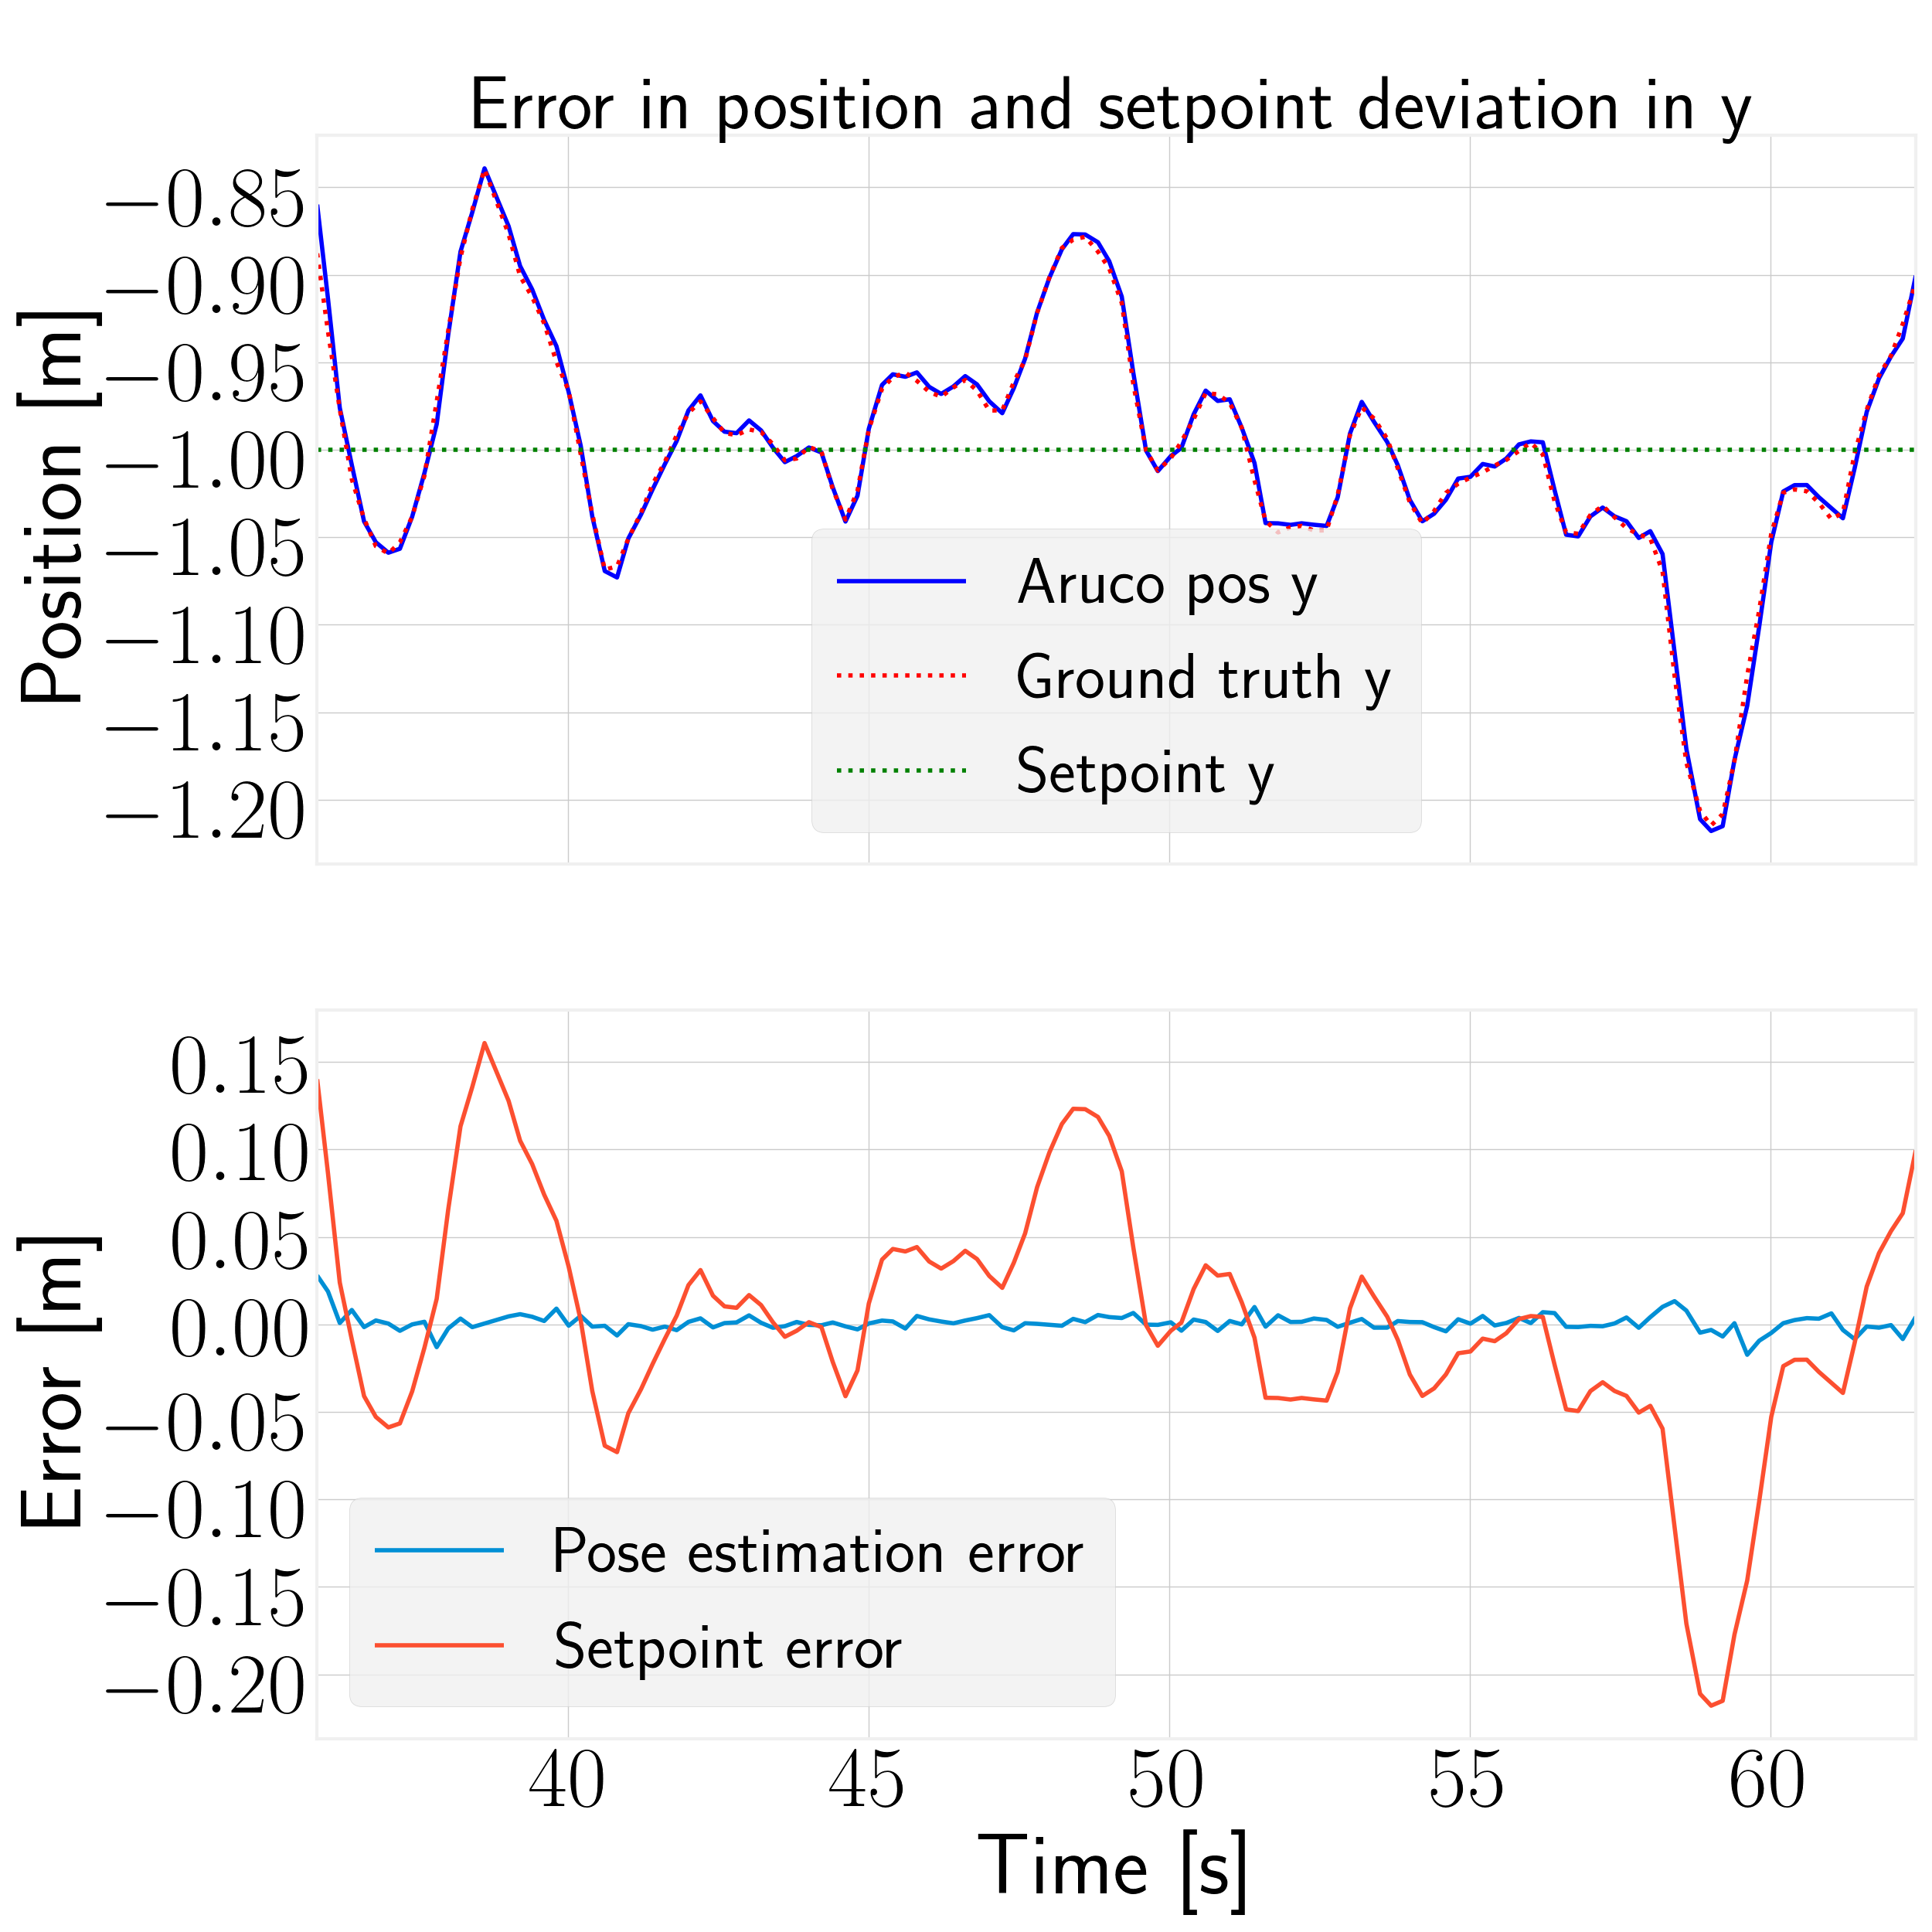
\includegraphics[width=\textwidth]{../Figures//hold_pose_using_aruco_pose_estimation/test2_gps2visionBoard_1.0Wind_-1.0y/error_y/pose_error_y_test1.png}
        \caption{}
        \label{fig:hold_pose_estimation_test2_y}
    \end{subfigure}
     \hspace{0.2em}
    \begin{subfigure}[t]{.30\textwidth}
        \centering
        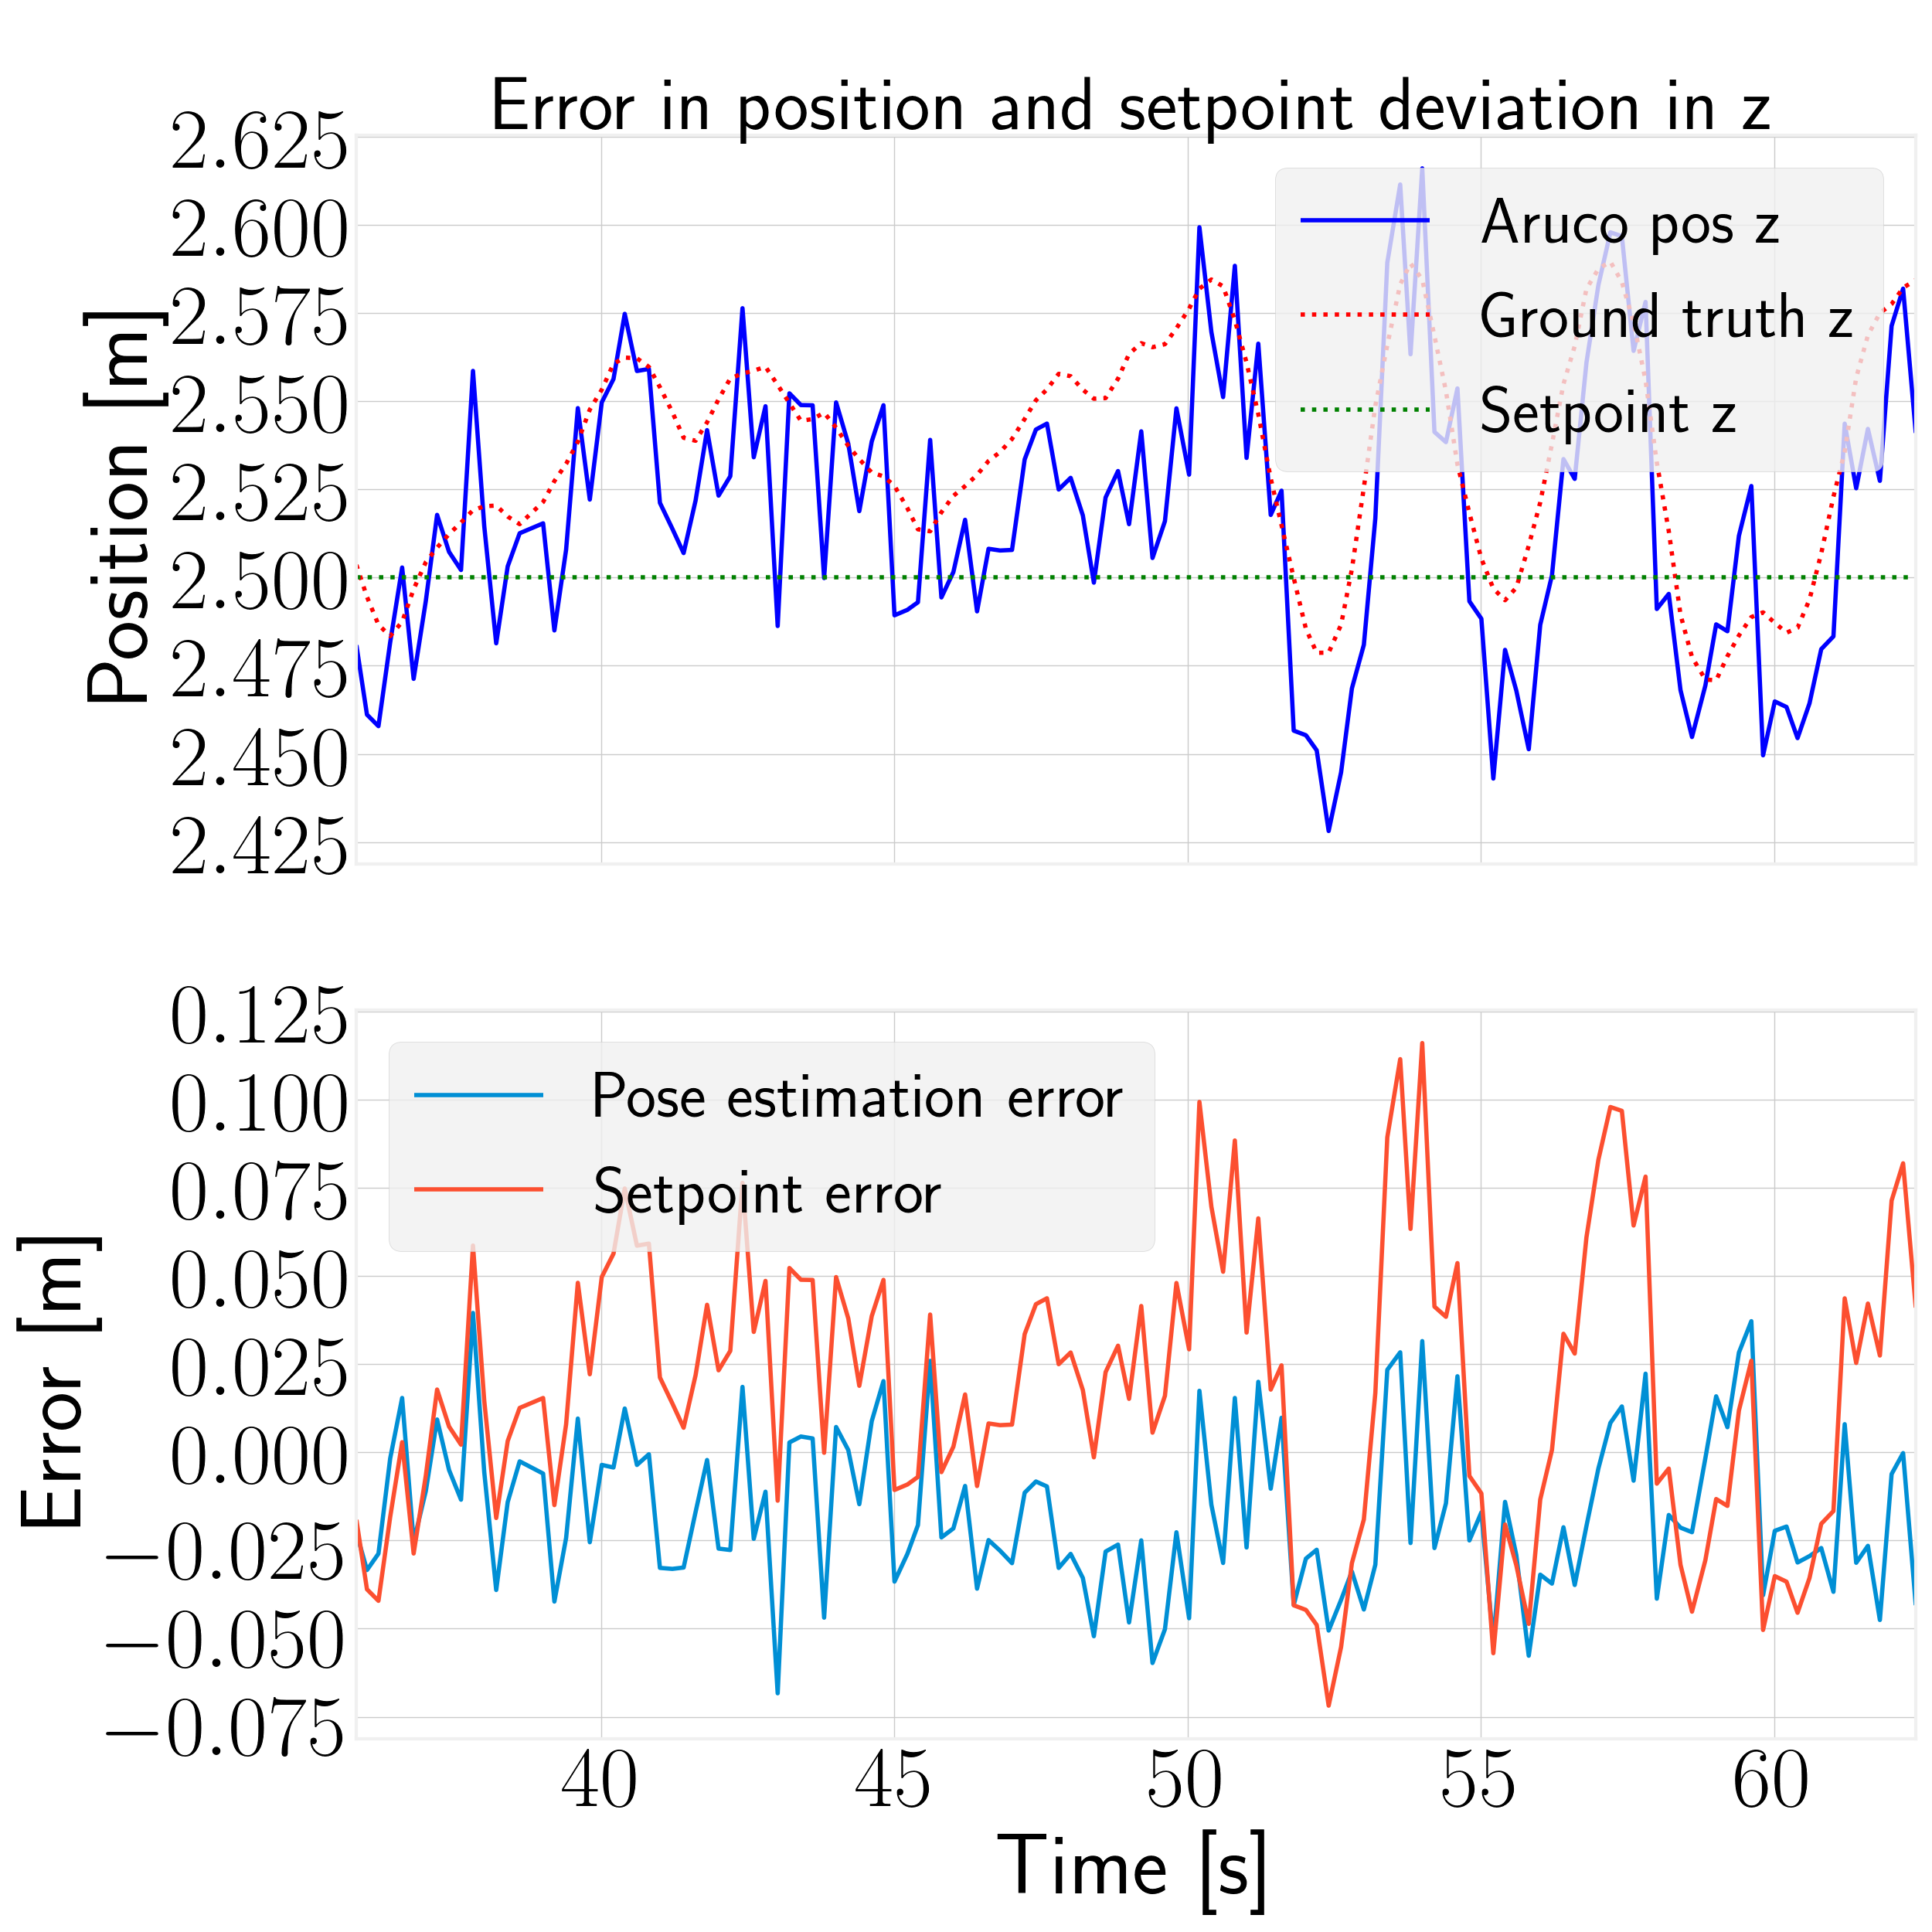
\includegraphics[width=\textwidth]{../Figures/hold_pose_using_aruco_pose_estimation/test2_gps2visionBoard_1.0Wind_-1.0y/error_z/pose_error_z_test1.png}
        \caption{}
        \label{fig:hold_pose_estimation_test2_z}
    \end{subfigure}
    \caption{}
    \label{fig:hold_pose_estimation_test2_error_pos}
\end{figure}

\begin{figure}[H]
    \centering
    \begin{subfigure}[t]{.30\textwidth}
        \centering
        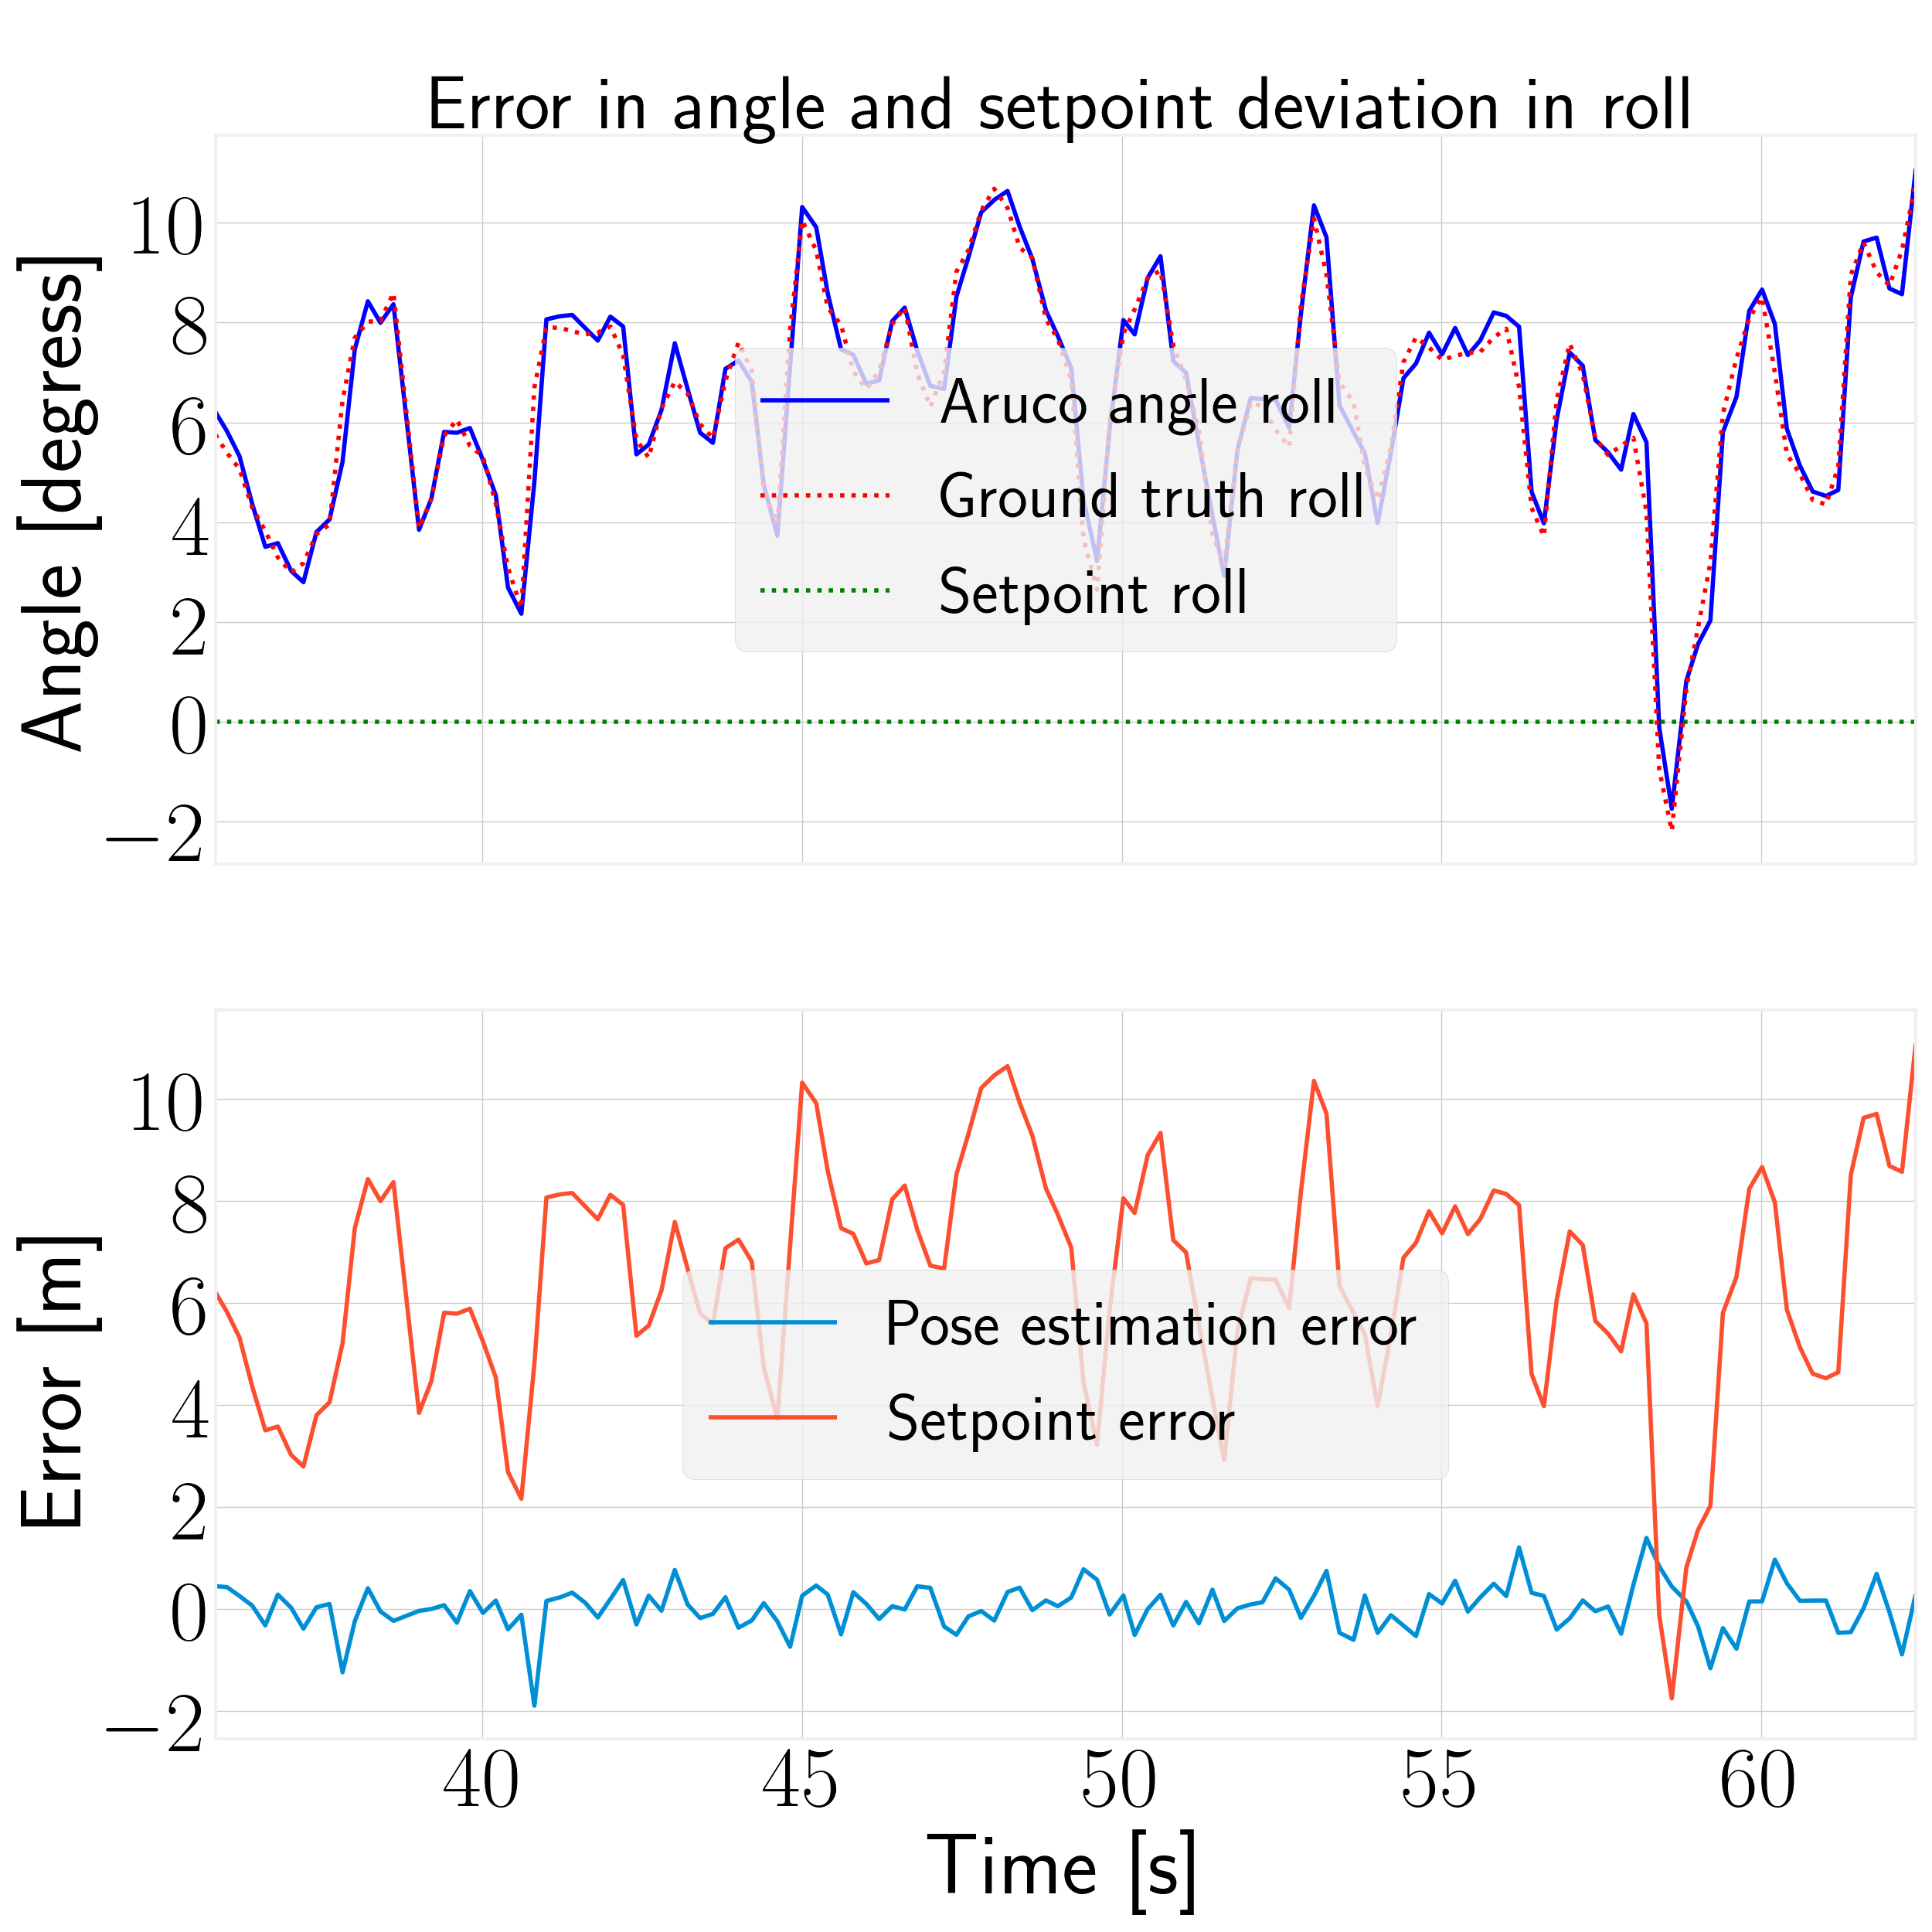
\includegraphics[width=\textwidth]{../Figures/hold_pose_using_aruco_pose_estimation/test2_gps2visionBoard_1.0Wind_-1.0y/error_roll/pose_error_roll_test1.png}
        \caption{}
        \label{fig:hold_pose_estimation_test2_roll}
    \end{subfigure}
     \hspace{0.2em}
    \begin{subfigure}[t]{.30\textwidth}
        \centering
        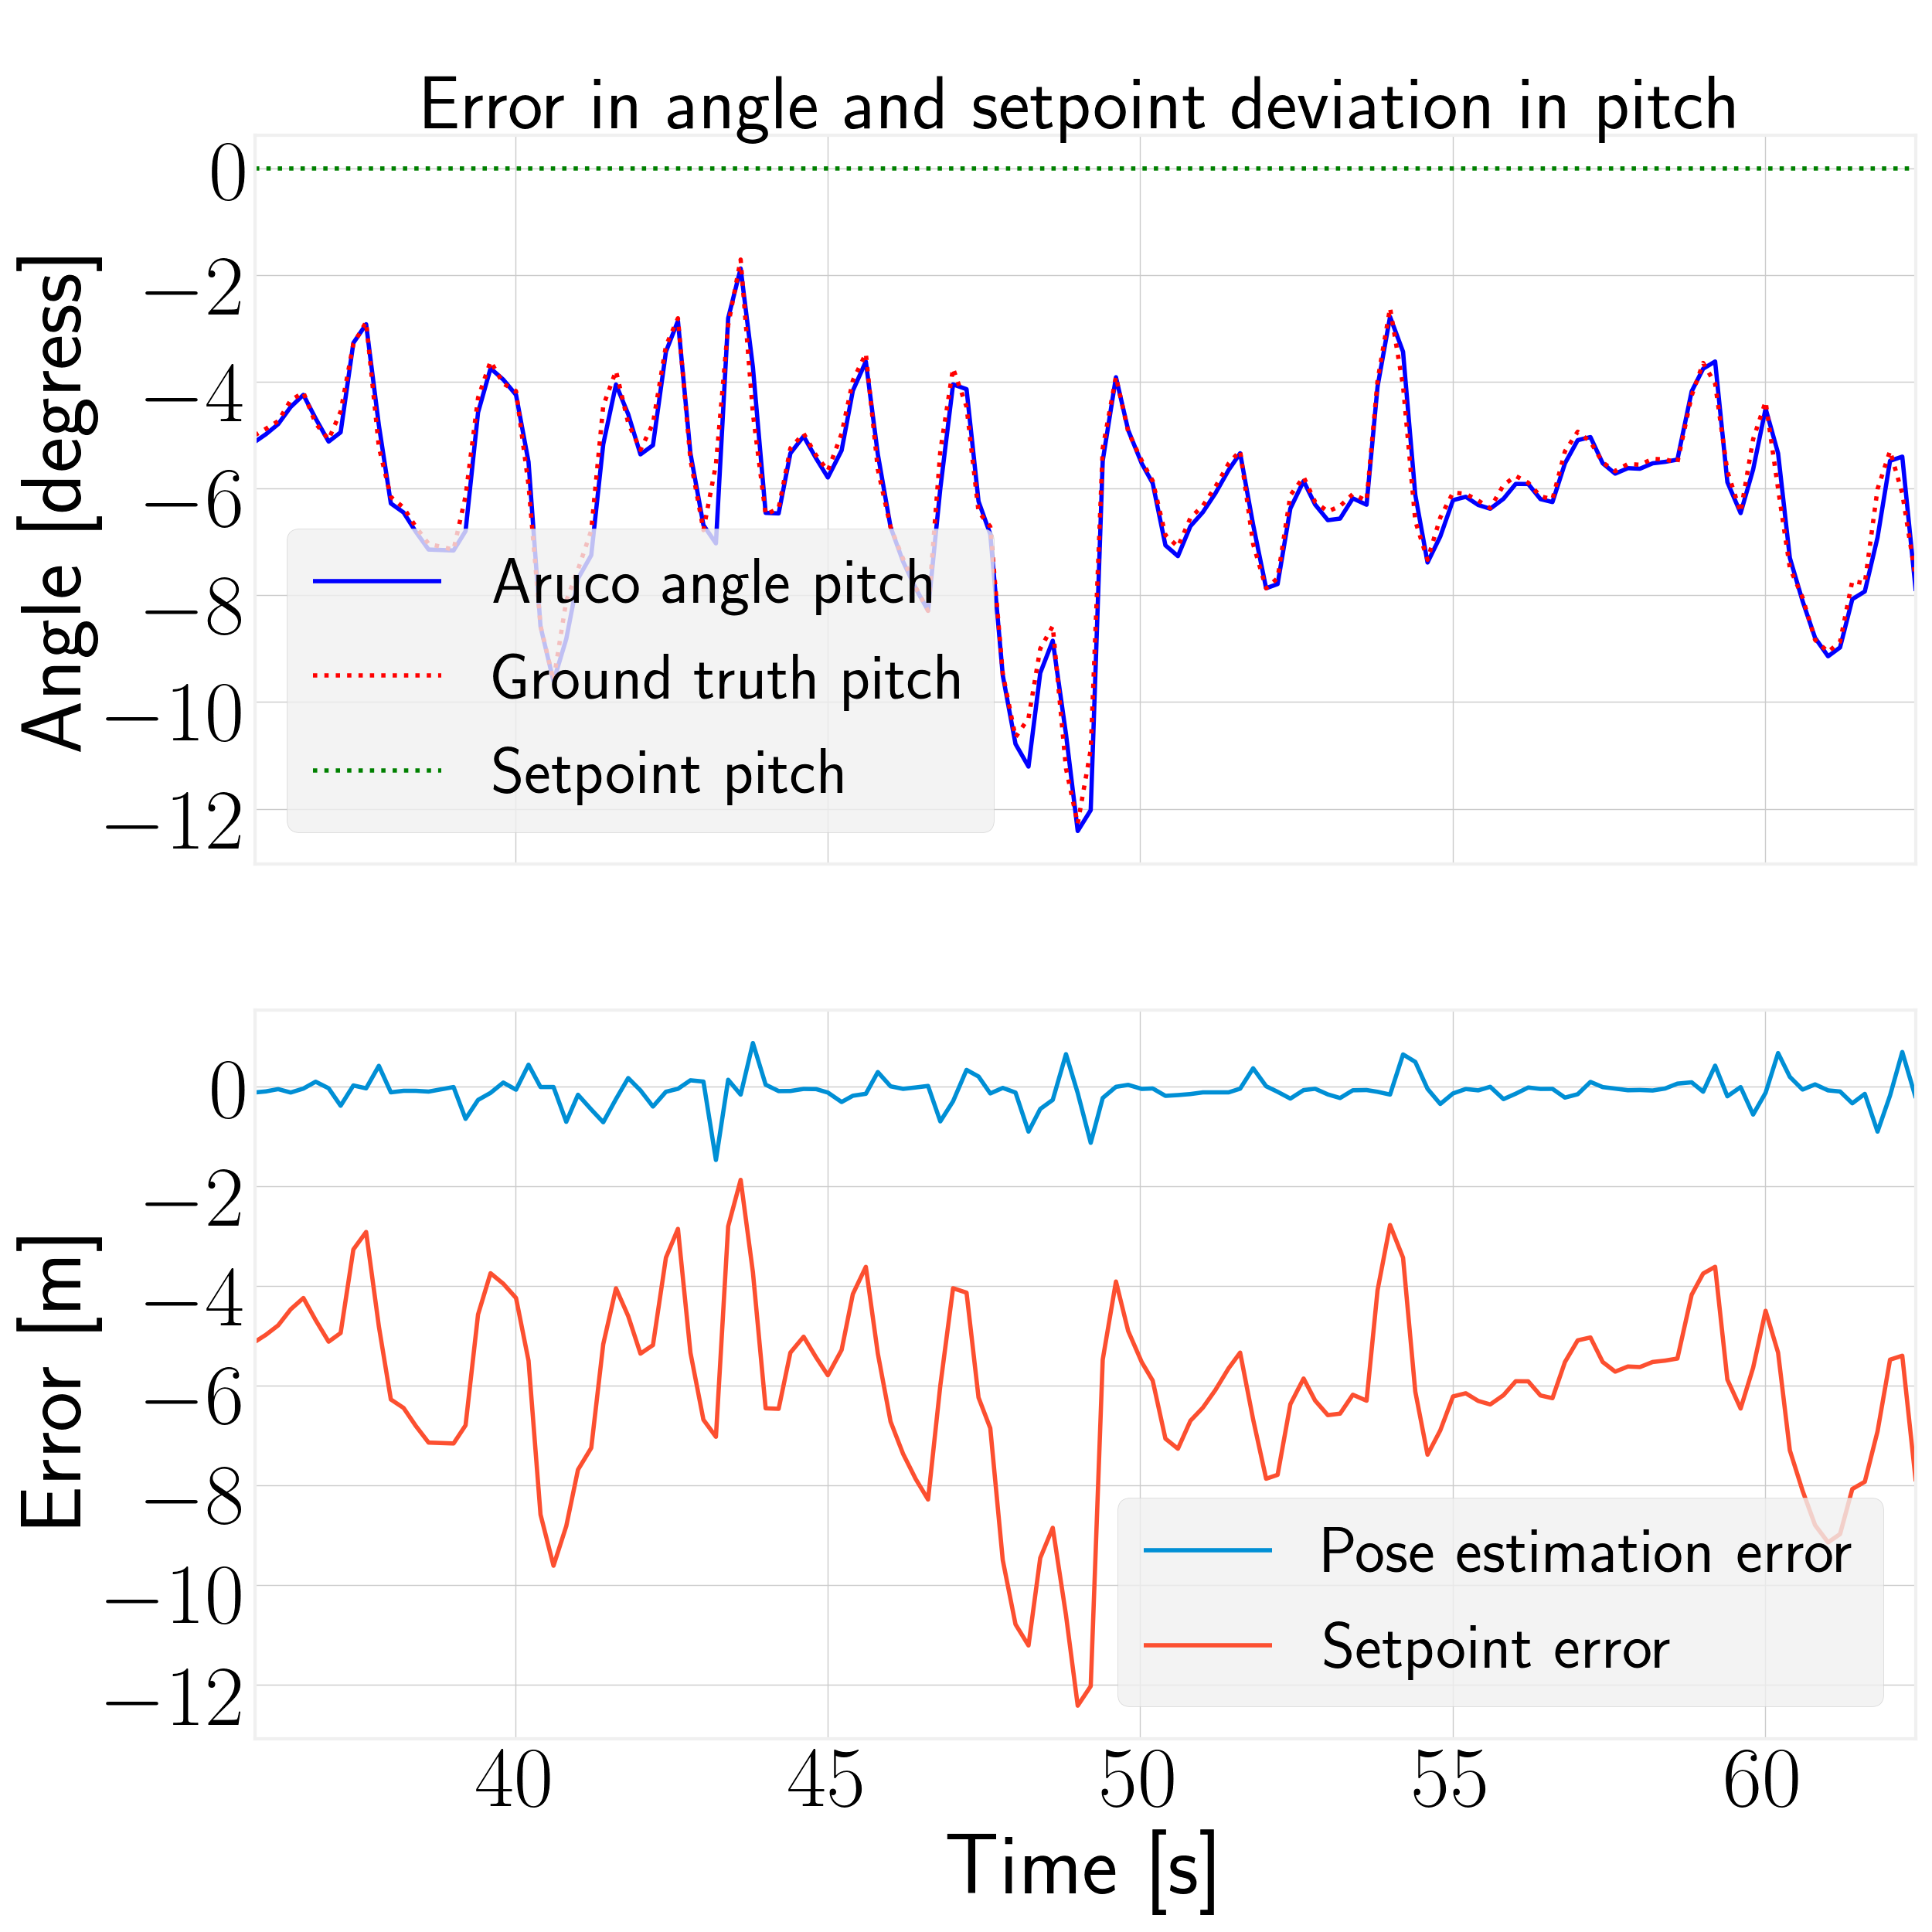
\includegraphics[width=\textwidth]{../Figures//hold_pose_using_aruco_pose_estimation/test2_gps2visionBoard_1.0Wind_-1.0y/error_pitch/pose_error_pitch_test1.png}
        \caption{}
        \label{fig:hold_pose_estimation_test2_pitch}
    \end{subfigure}
     \hspace{0.2em}
    \begin{subfigure}[t]{.30\textwidth}
        \centering
        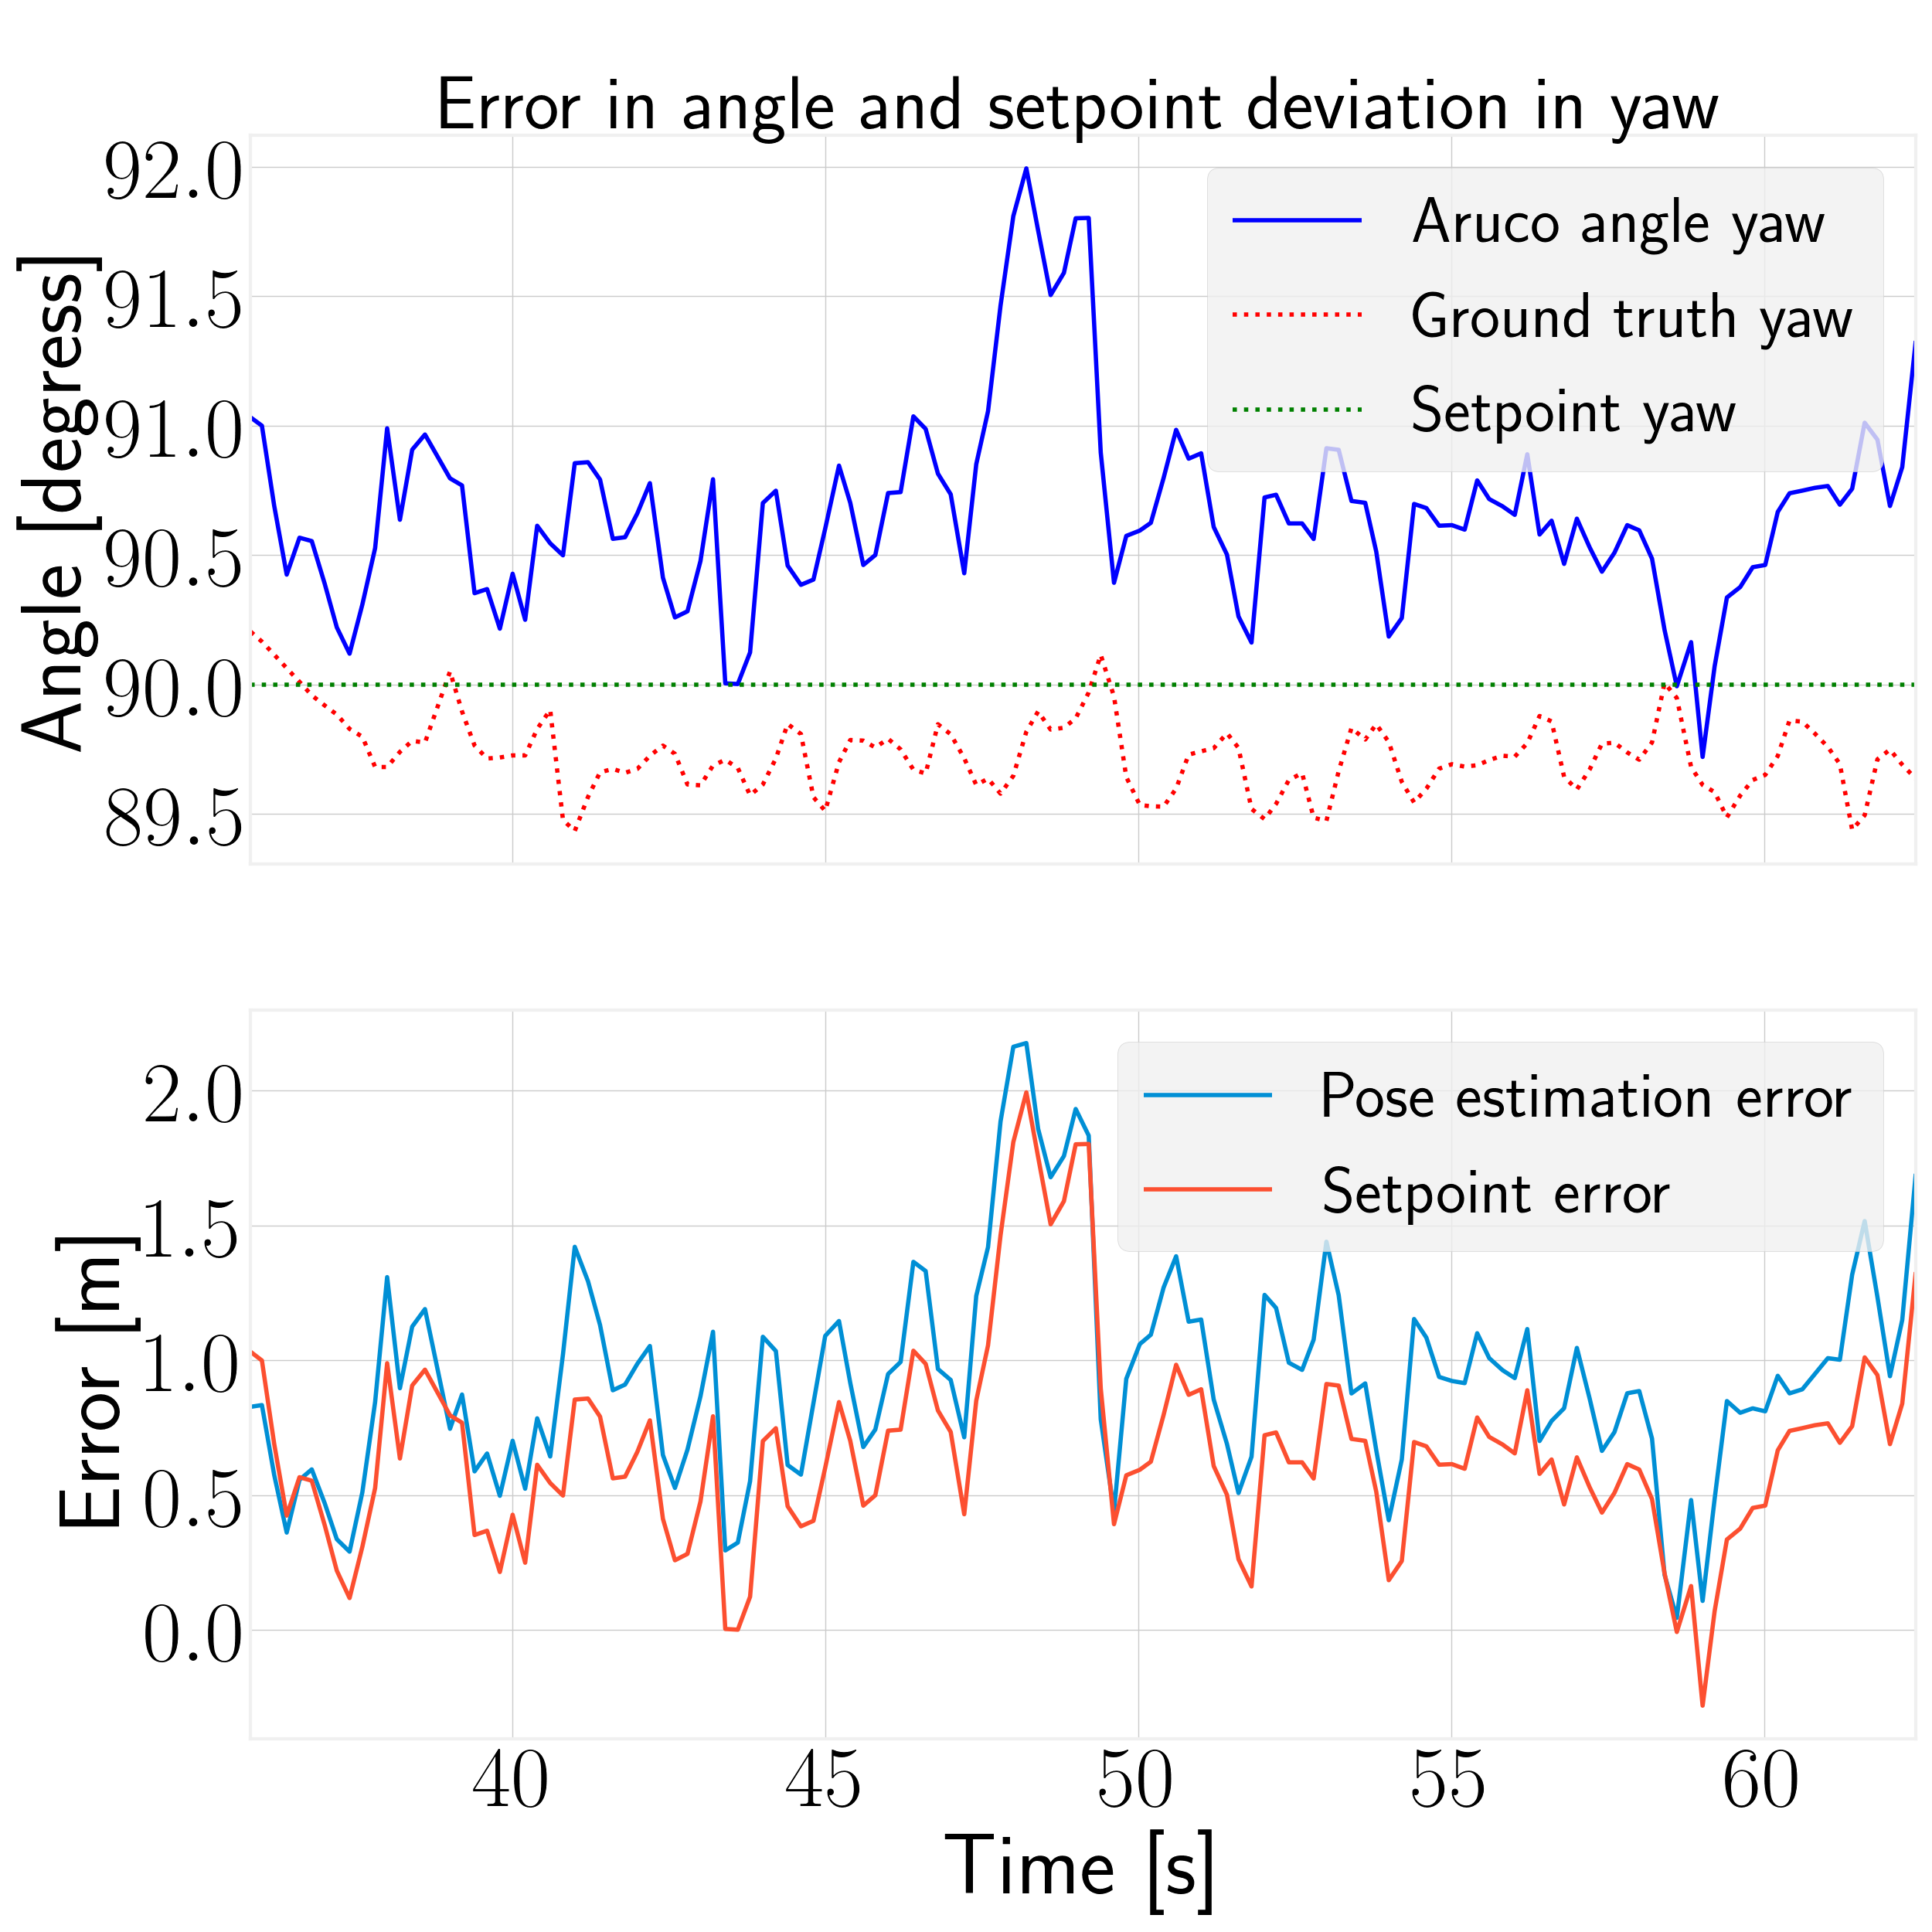
\includegraphics[width=\textwidth]{../Figures/hold_pose_using_aruco_pose_estimation/test2_gps2visionBoard_1.0Wind_-1.0y/error_yaw/pose_error_yaw_test1.png}
        \caption{}
        \label{fig:hold_pose_estimation_test2_yaw}
    \end{subfigure}
    \caption{}
    \label{fig:hold_pose_estimation_test2_error_angle}
\end{figure}

\begin{figure}[H]
    \centering
    \begin{subfigure}[t]{.30\textwidth}
        \centering
        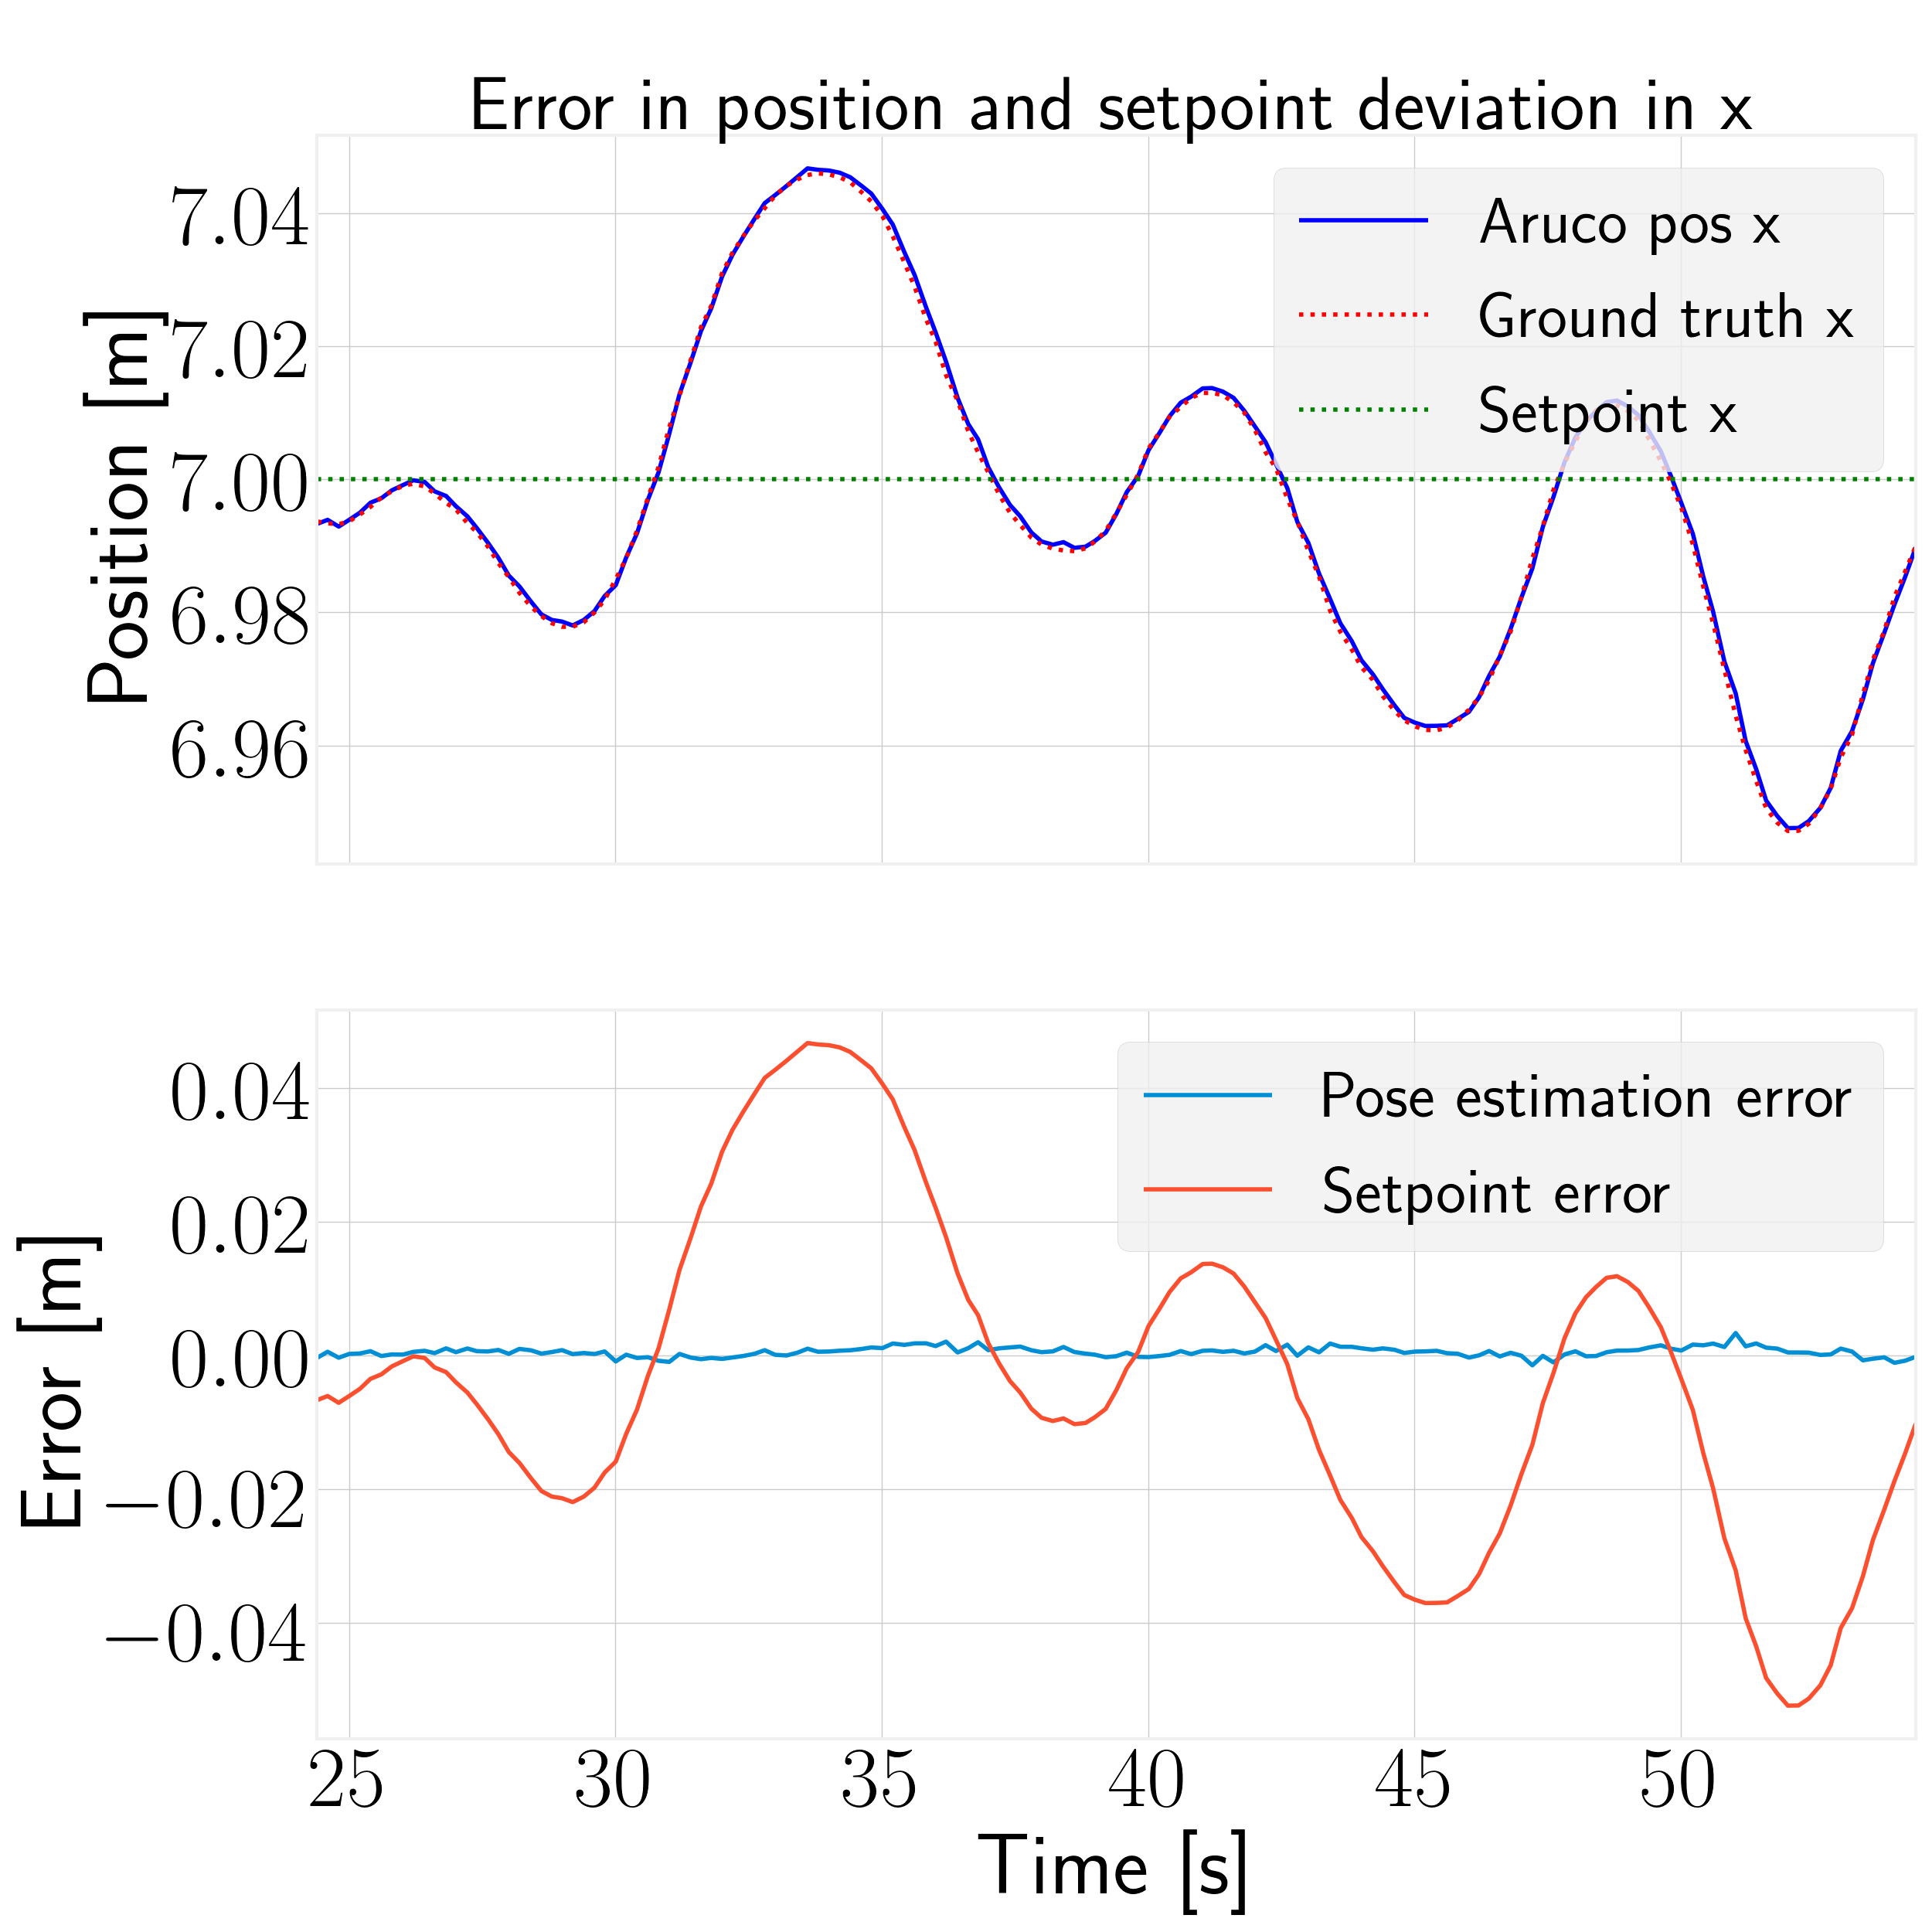
\includegraphics[width=\textwidth]{../Figures/hold_pose_using_aruco_pose_estimation/test5_landingBoard3_noWind/error_x/pose_error_x_test1.png}
        \caption{}
        \label{fig:hold_pose_estimation_test5_x}
    \end{subfigure}
     \hspace{0.2em}
    \begin{subfigure}[t]{.30\textwidth}
        \centering
        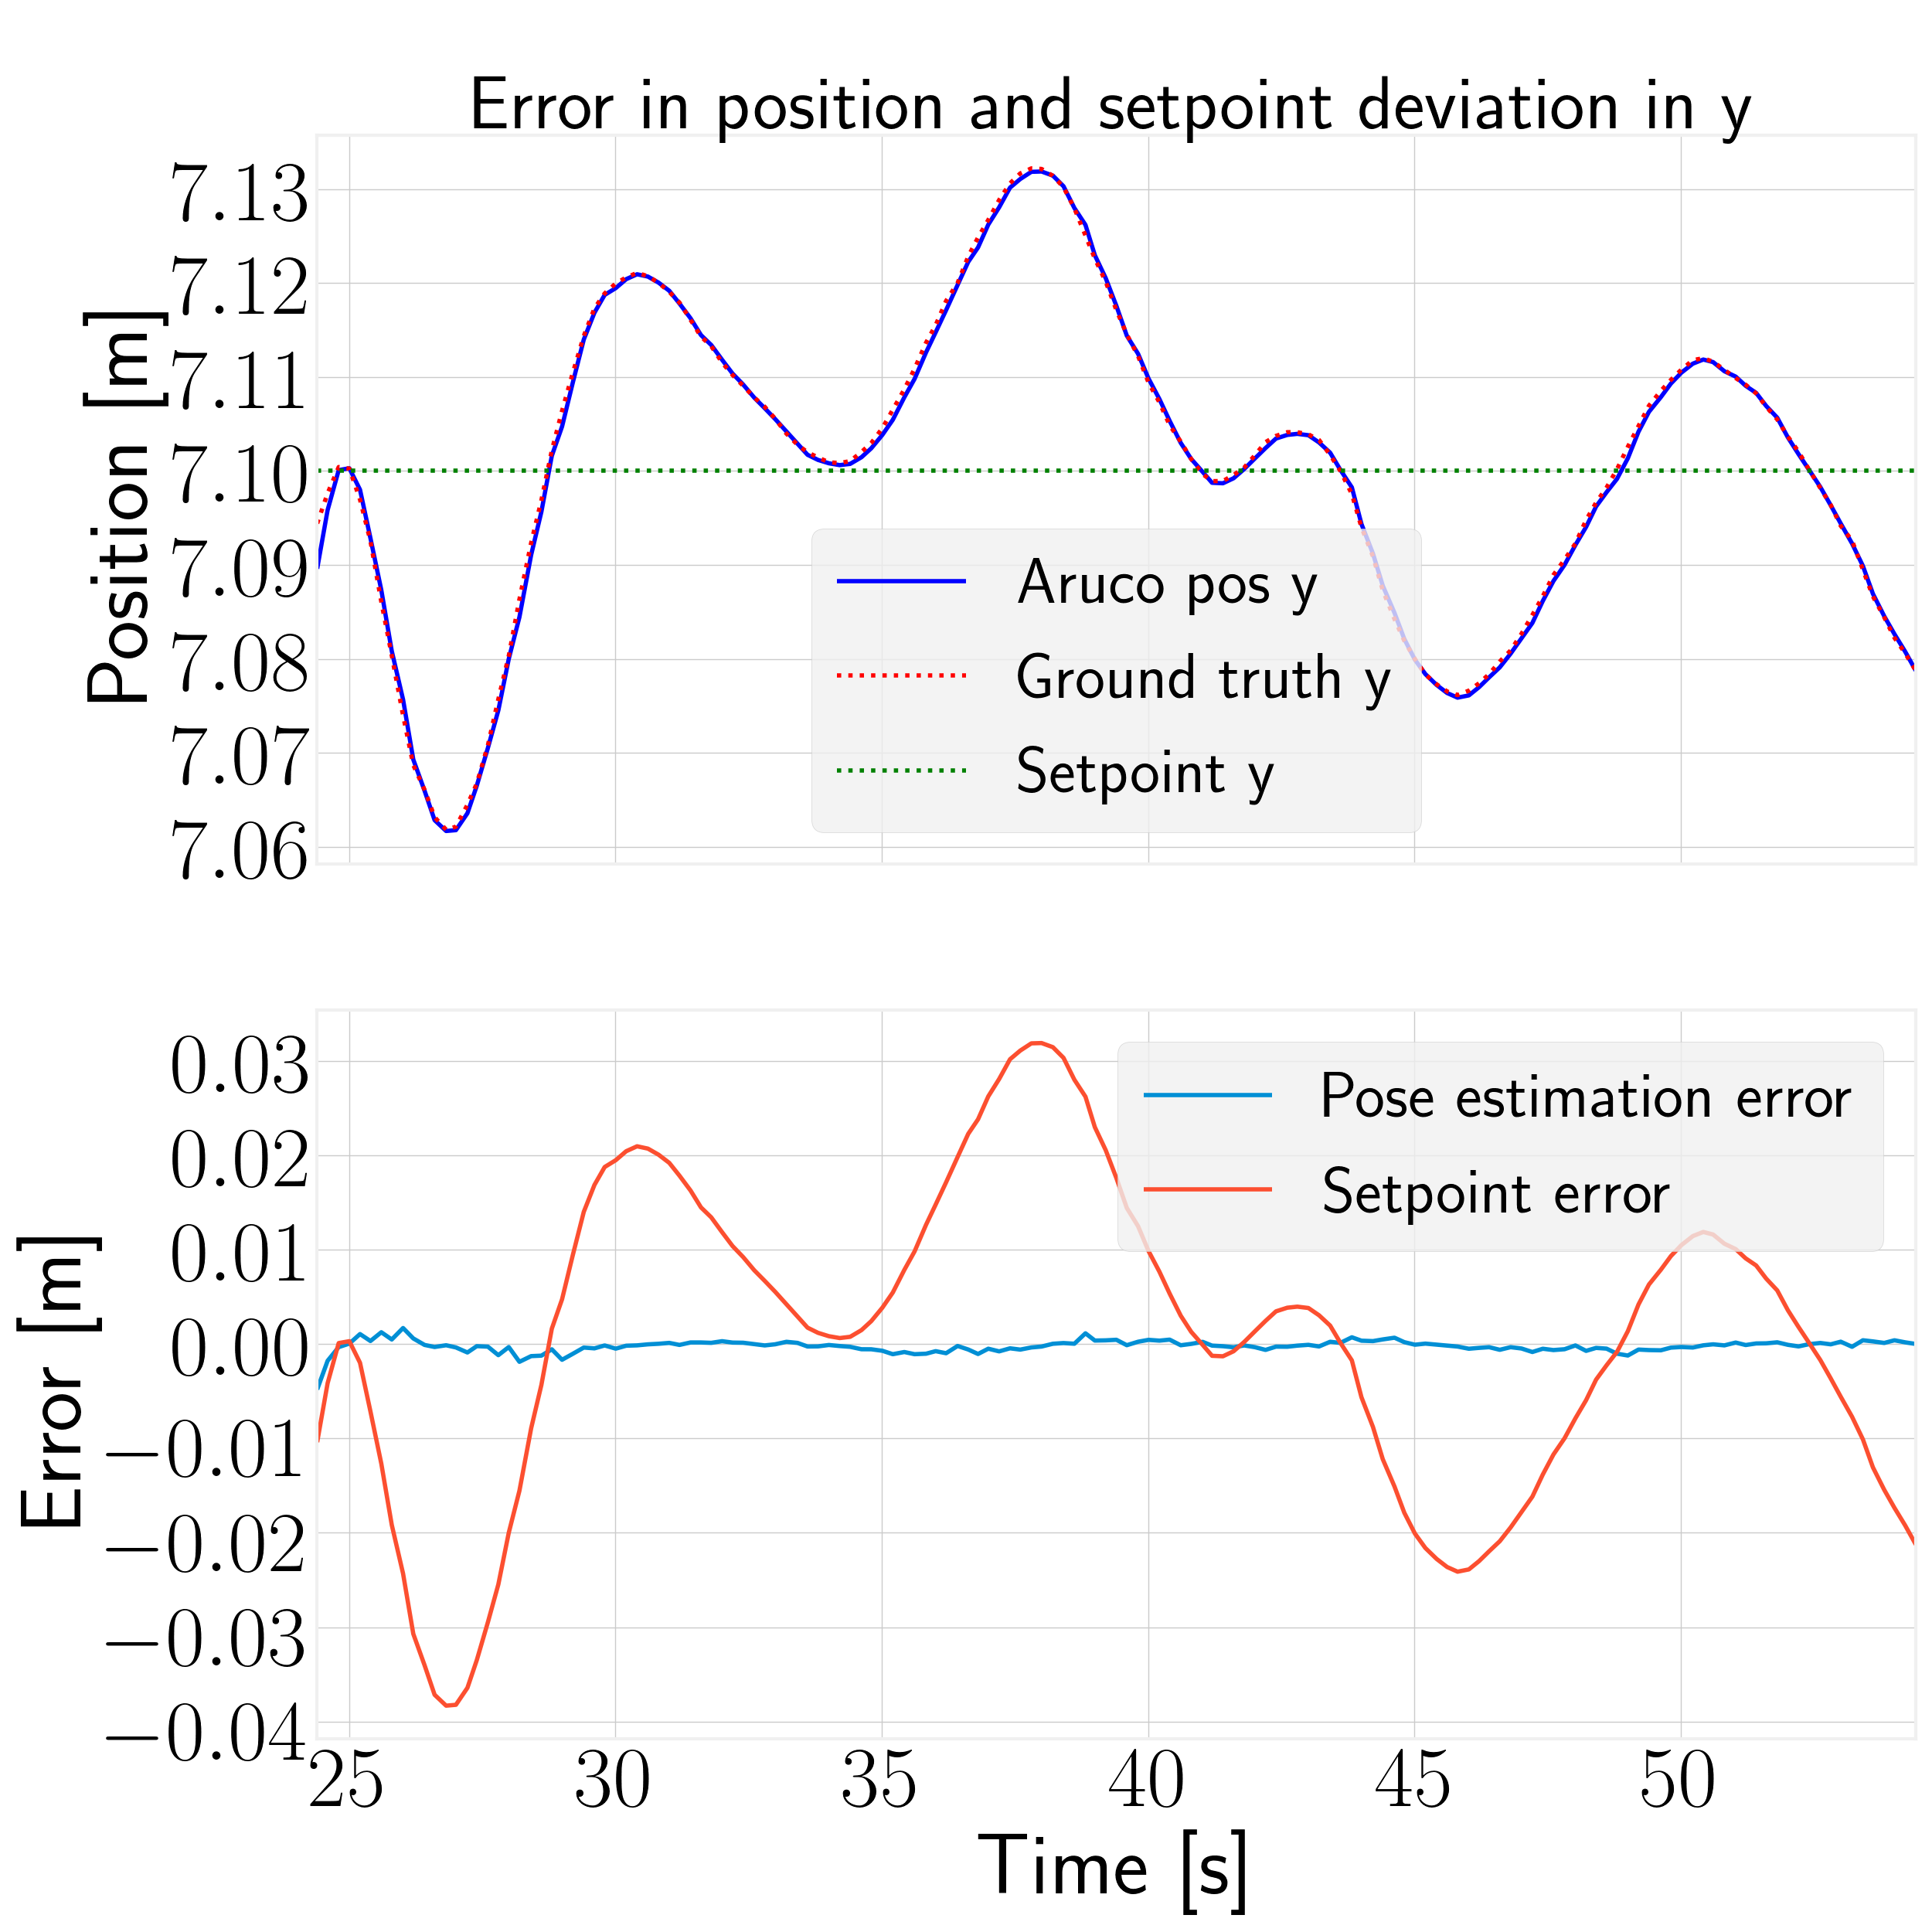
\includegraphics[width=\textwidth]{../Figures//hold_pose_using_aruco_pose_estimation/test5_landingBoard3_noWind/error_y/pose_error_y_test1.png}
        \caption{}
        \label{fig:hold_pose_estimation_test5_y}
    \end{subfigure}
     \hspace{0.2em}
    \begin{subfigure}[t]{.30\textwidth}
        \centering
        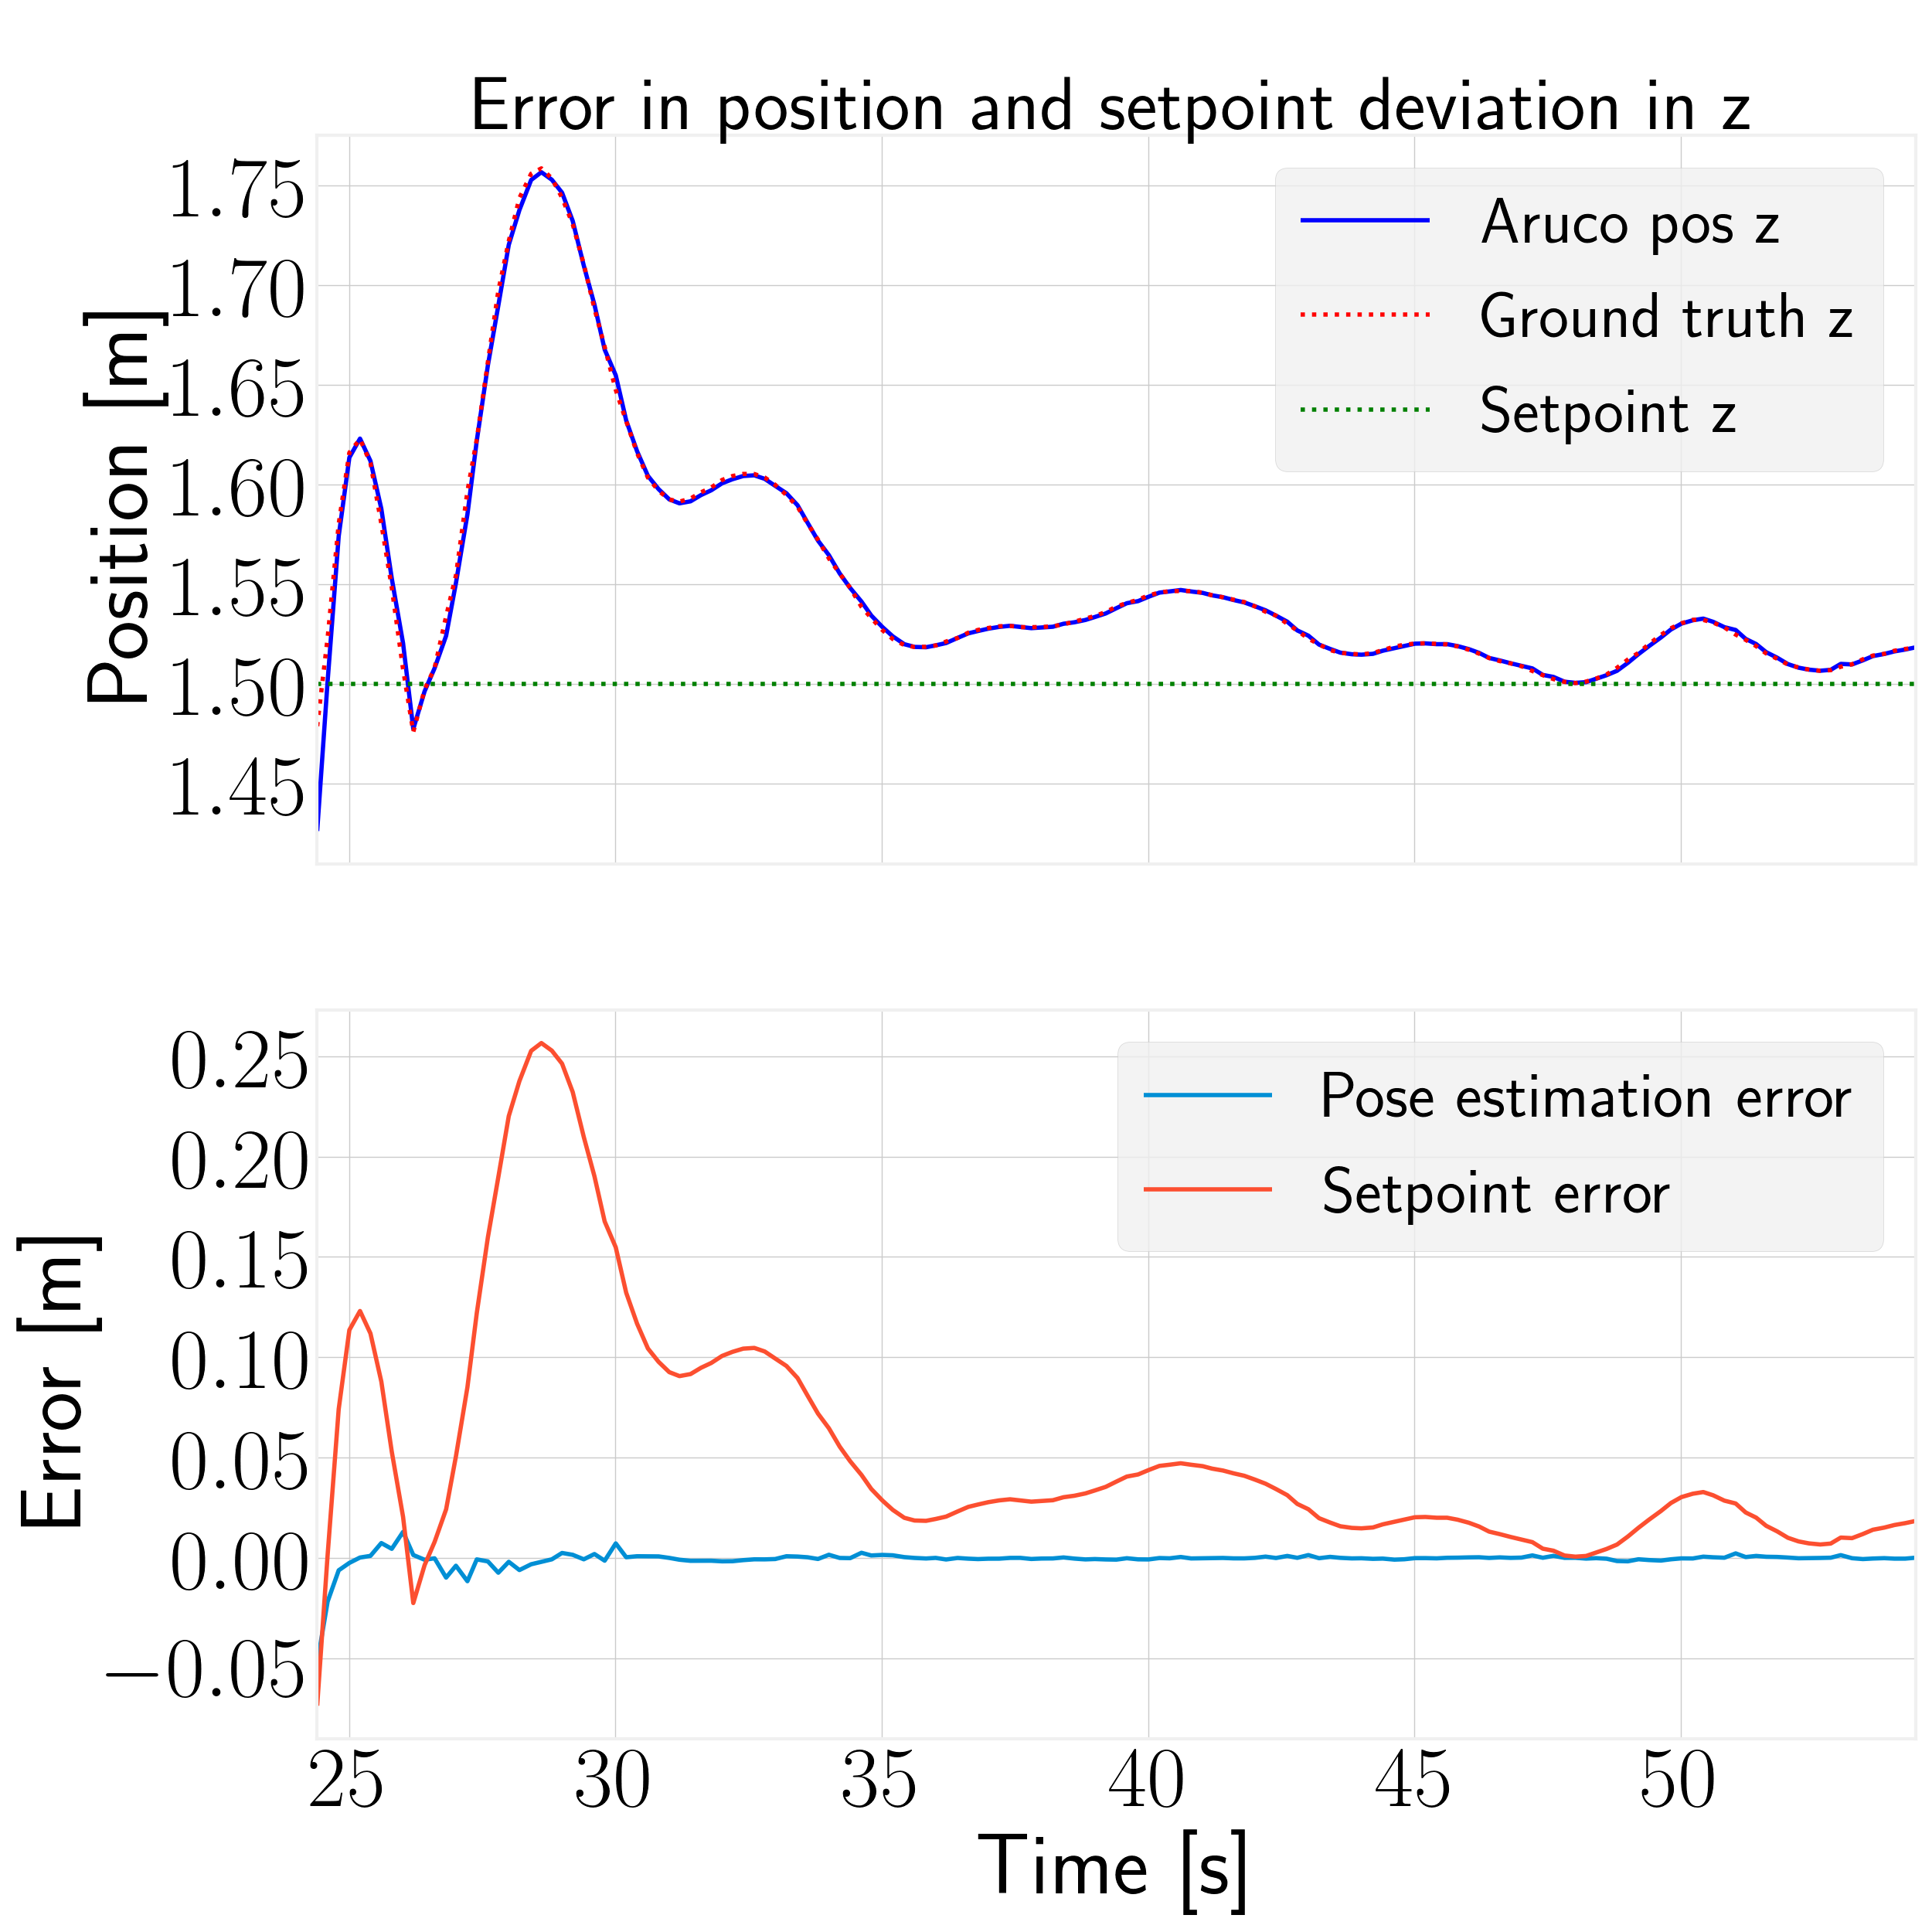
\includegraphics[width=\textwidth]{../Figures/hold_pose_using_aruco_pose_estimation/test5_landingBoard3_noWind/error_z/pose_error_z_test1.png}
        \caption{}
        \label{fig:hold_pose_estimation_test5_z}
    \end{subfigure}
    \caption{}
    \label{fig:hold_pose_estimation_test5_error_pos}
\end{figure}

\begin{figure}[H]
    \centering
    \begin{subfigure}[t]{.30\textwidth}
        \centering
        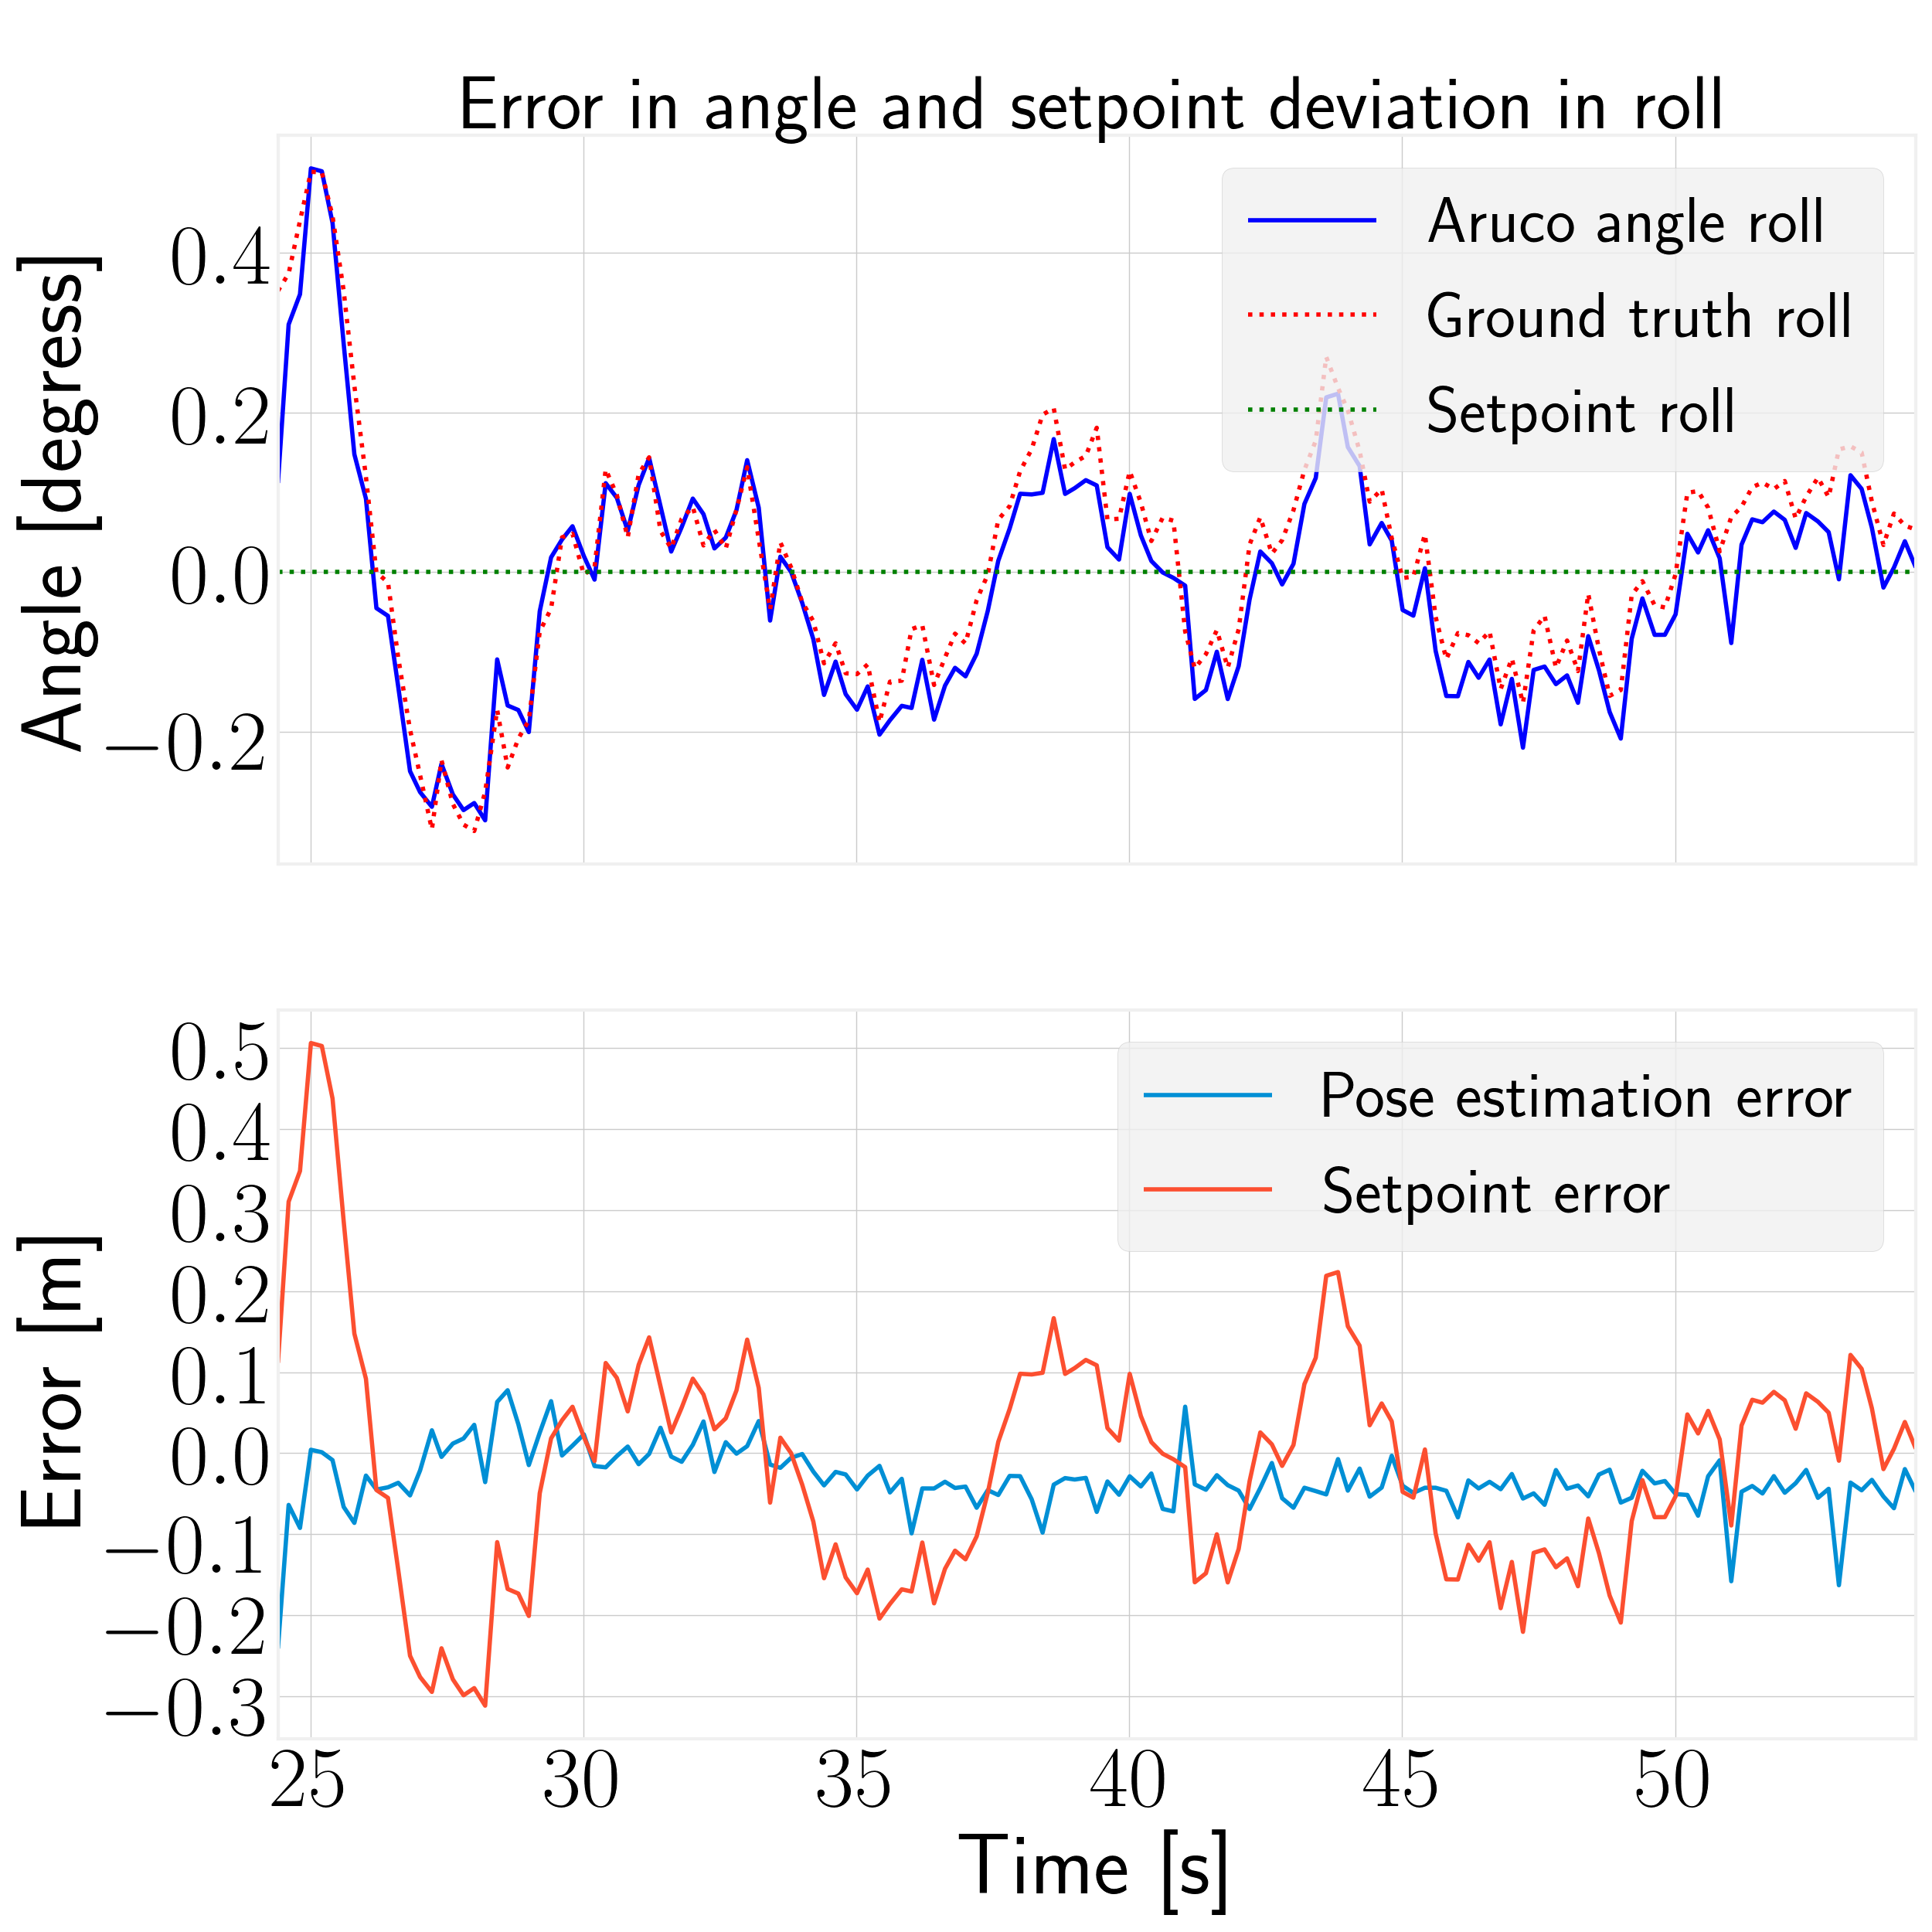
\includegraphics[width=\textwidth]{../Figures/hold_pose_using_aruco_pose_estimation/test5_landingBoard3_noWind/error_roll/pose_error_roll_test1.png}
        \caption{}
        \label{fig:hold_pose_estimation_test5_roll}
    \end{subfigure}
     \hspace{0.2em}
    \begin{subfigure}[t]{.30\textwidth}
        \centering
        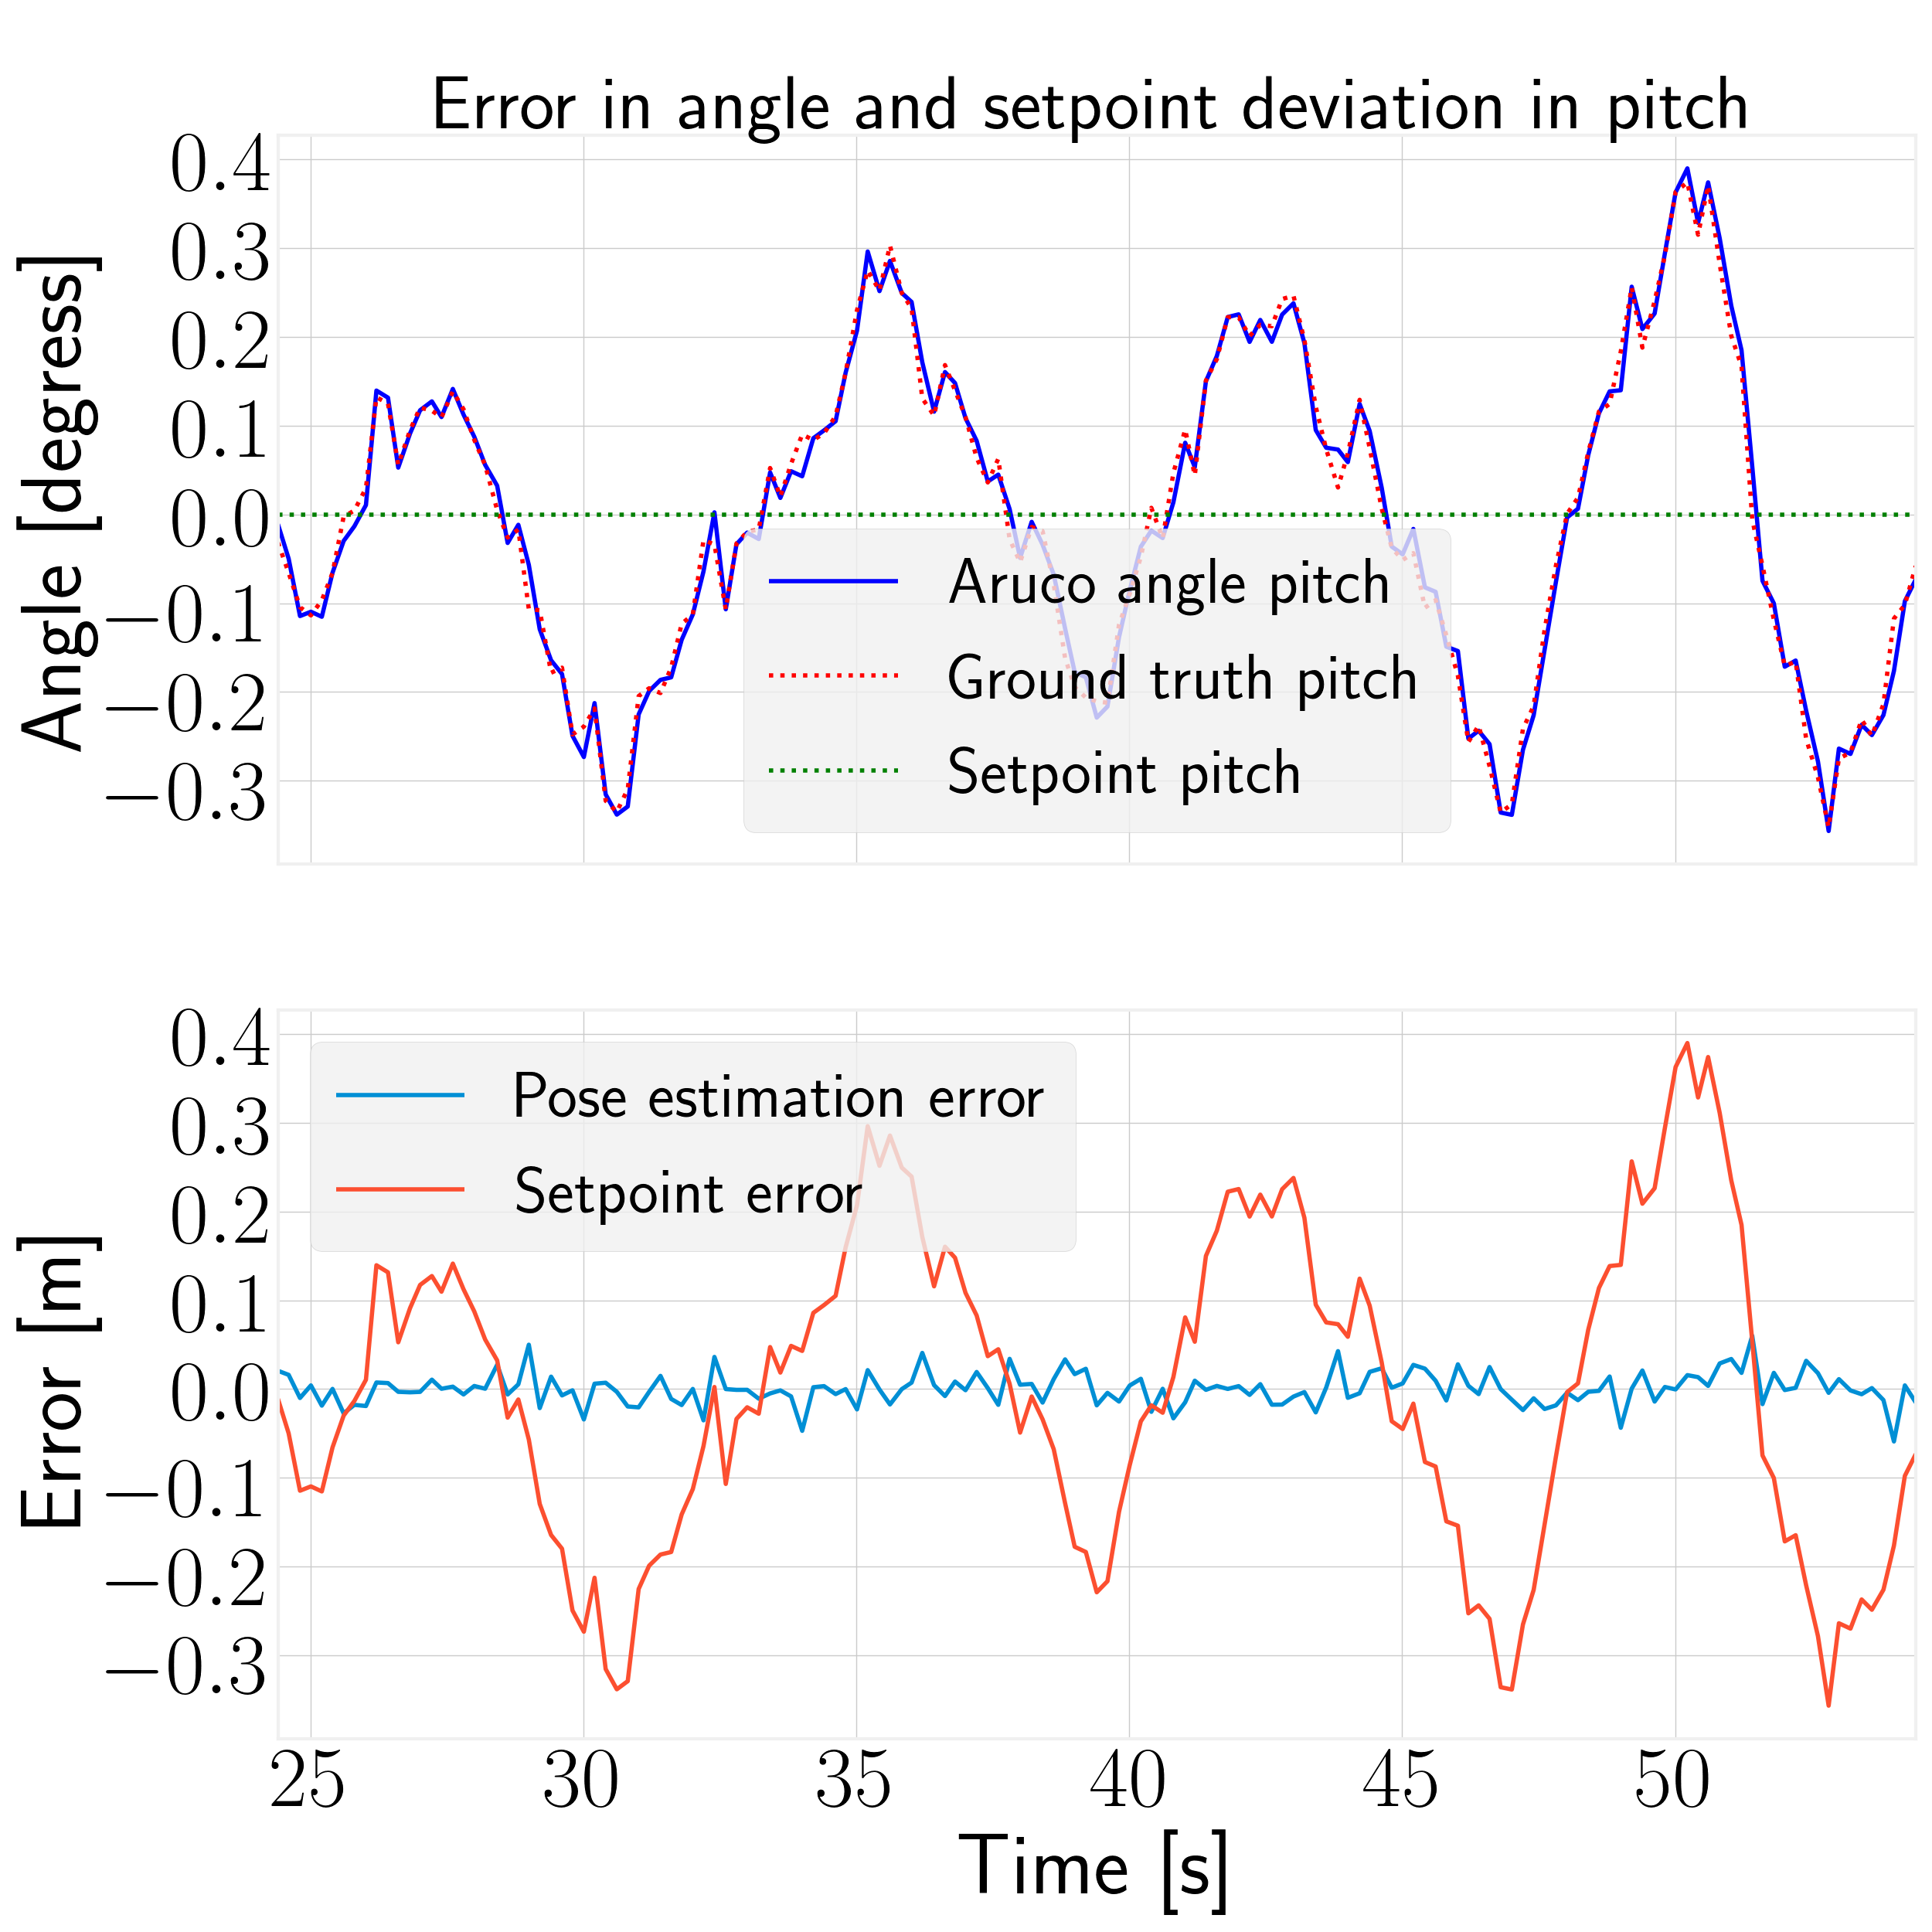
\includegraphics[width=\textwidth]{../Figures//hold_pose_using_aruco_pose_estimation/test5_landingBoard3_noWind/error_pitch/pose_error_pitch_test1.png}
        \caption{}
        \label{fig:hold_pose_estimation_test5_pitch}
    \end{subfigure}
     \hspace{0.2em}
    \begin{subfigure}[t]{.30\textwidth}
        \centering
        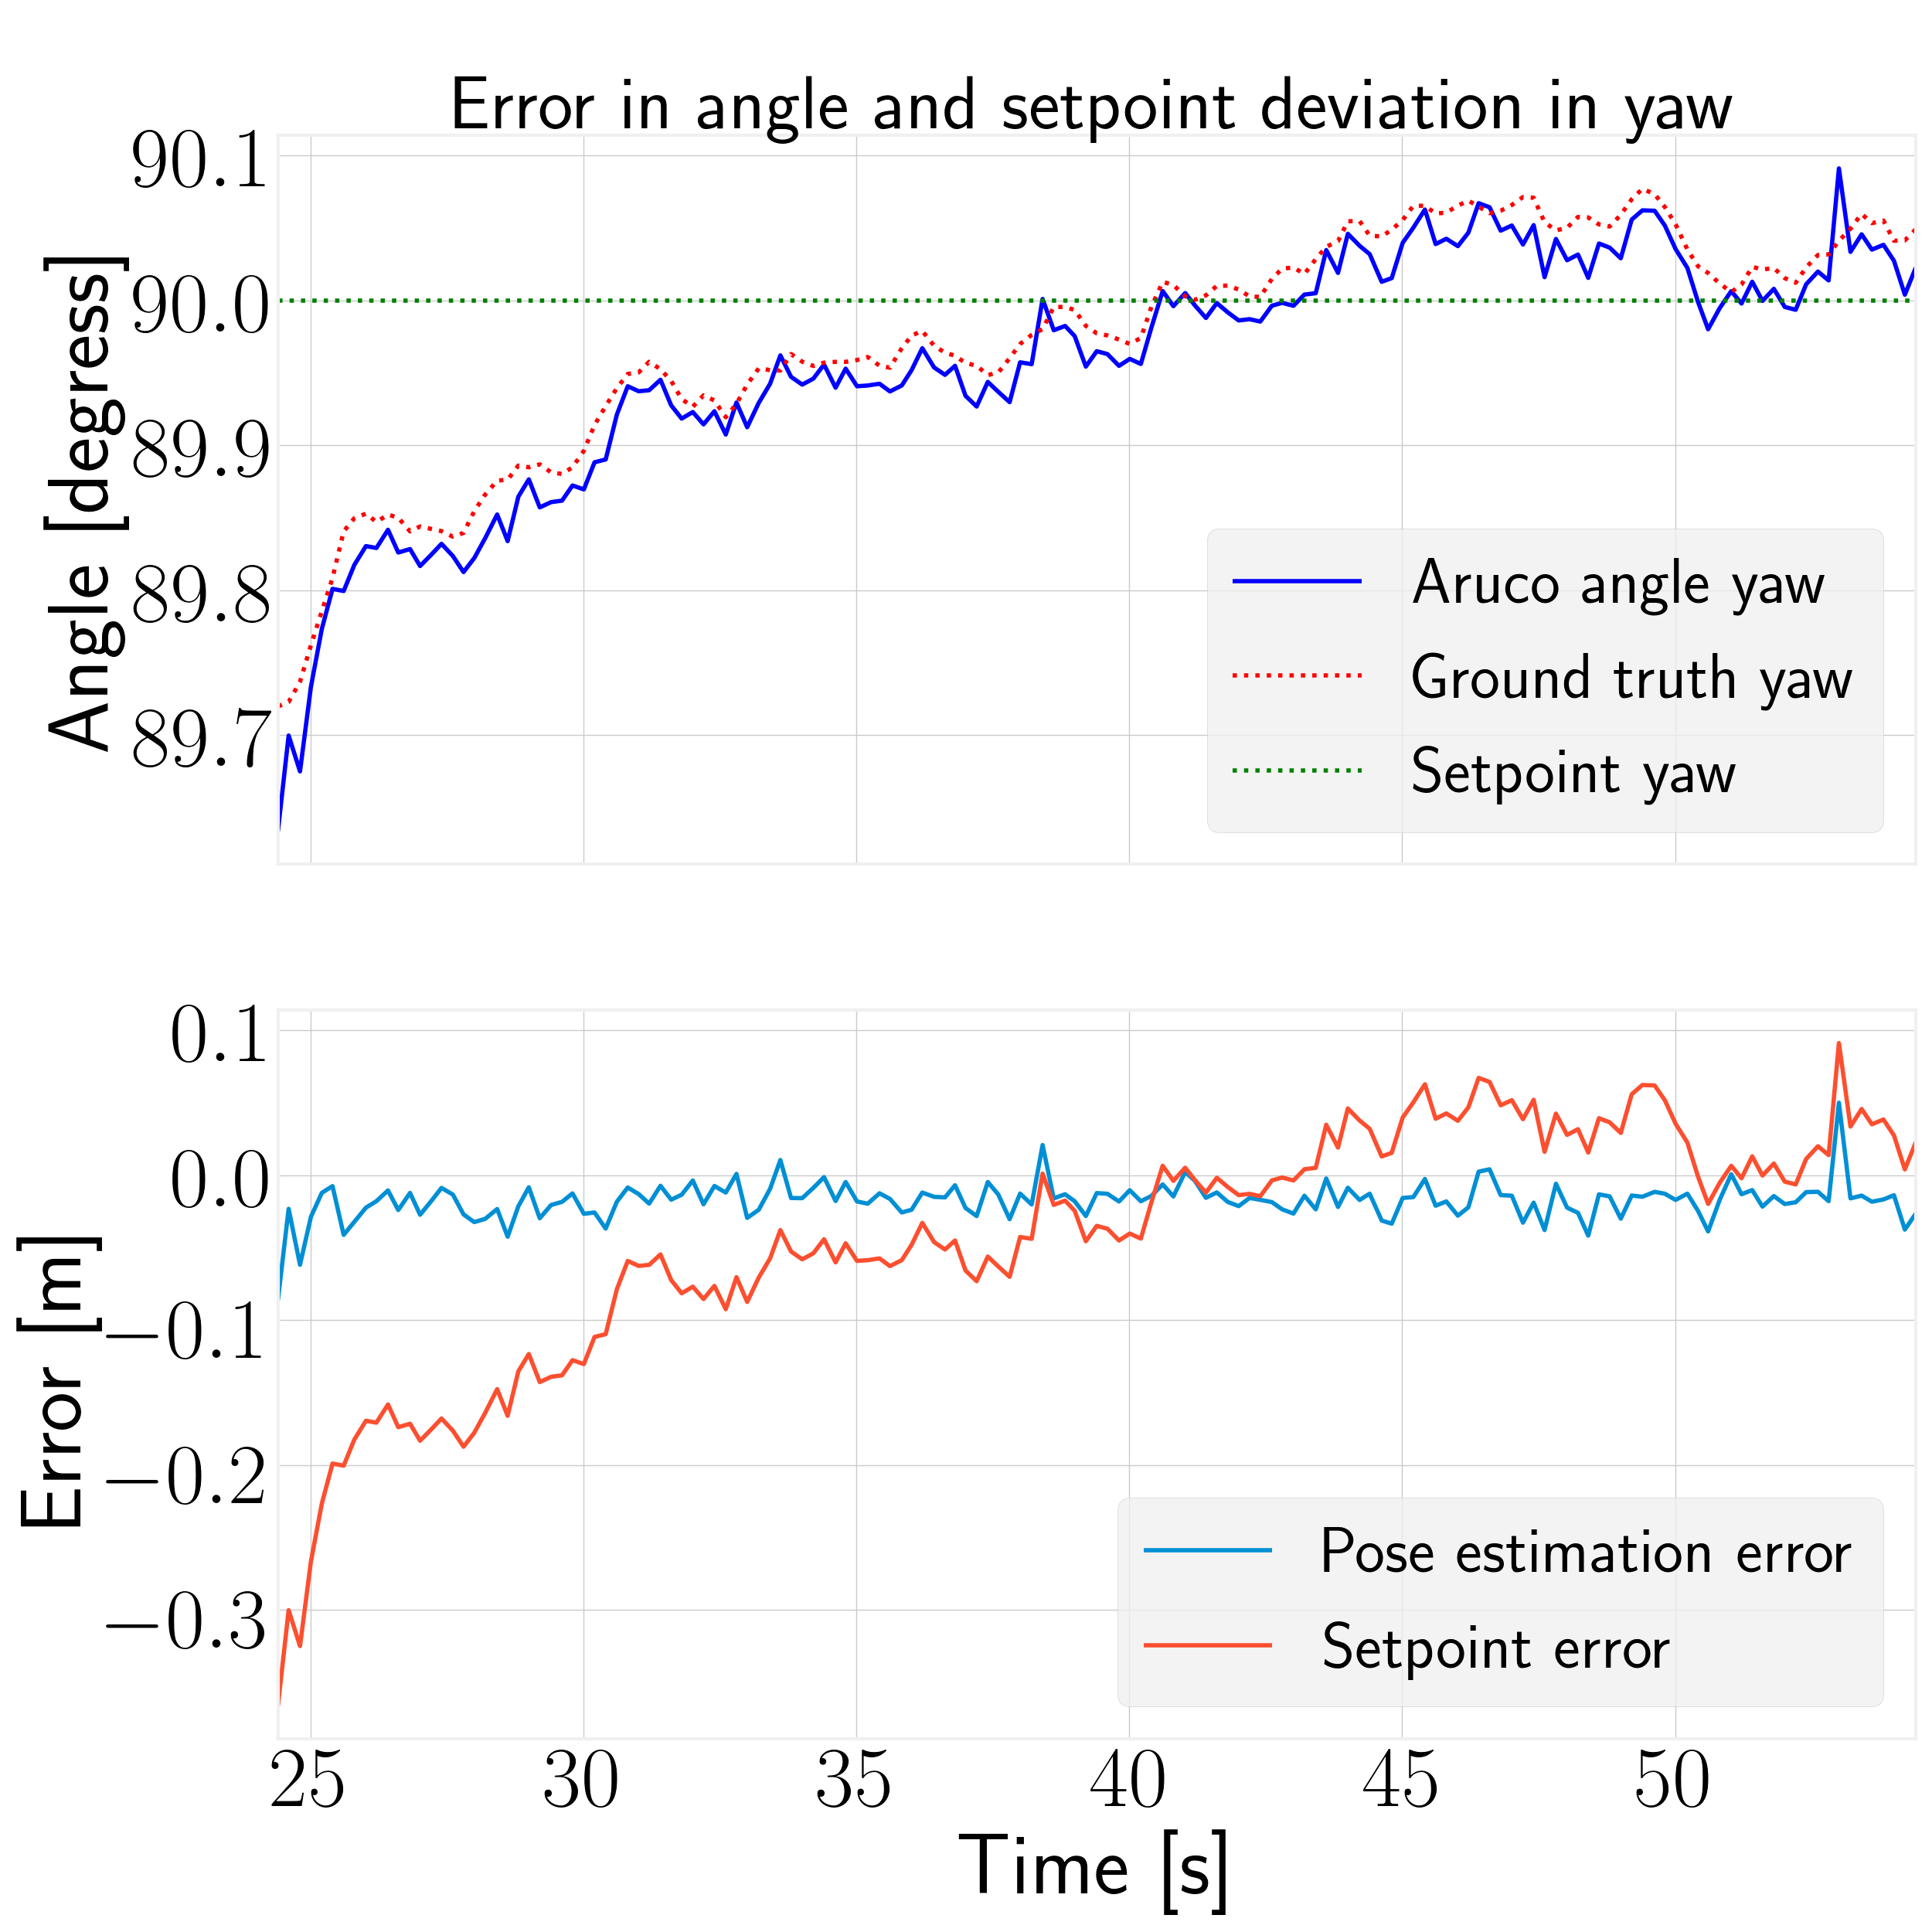
\includegraphics[width=\textwidth]{../Figures/hold_pose_using_aruco_pose_estimation/test5_landingBoard3_noWind/error_yaw/pose_error_yaw_test1.png}
        \caption{}
        \label{fig:hold_pose_estimation_test5_yaw}
    \end{subfigure}
    \caption{}
    \label{fig:hold_pose_estimation_test5_error_angle}
\end{figure}

\subsubsection{GPS to vision navigation}

\begin{figure}[H]
    \centering
    \begin{subfigure}[t]{.30\textwidth}
        \centering
        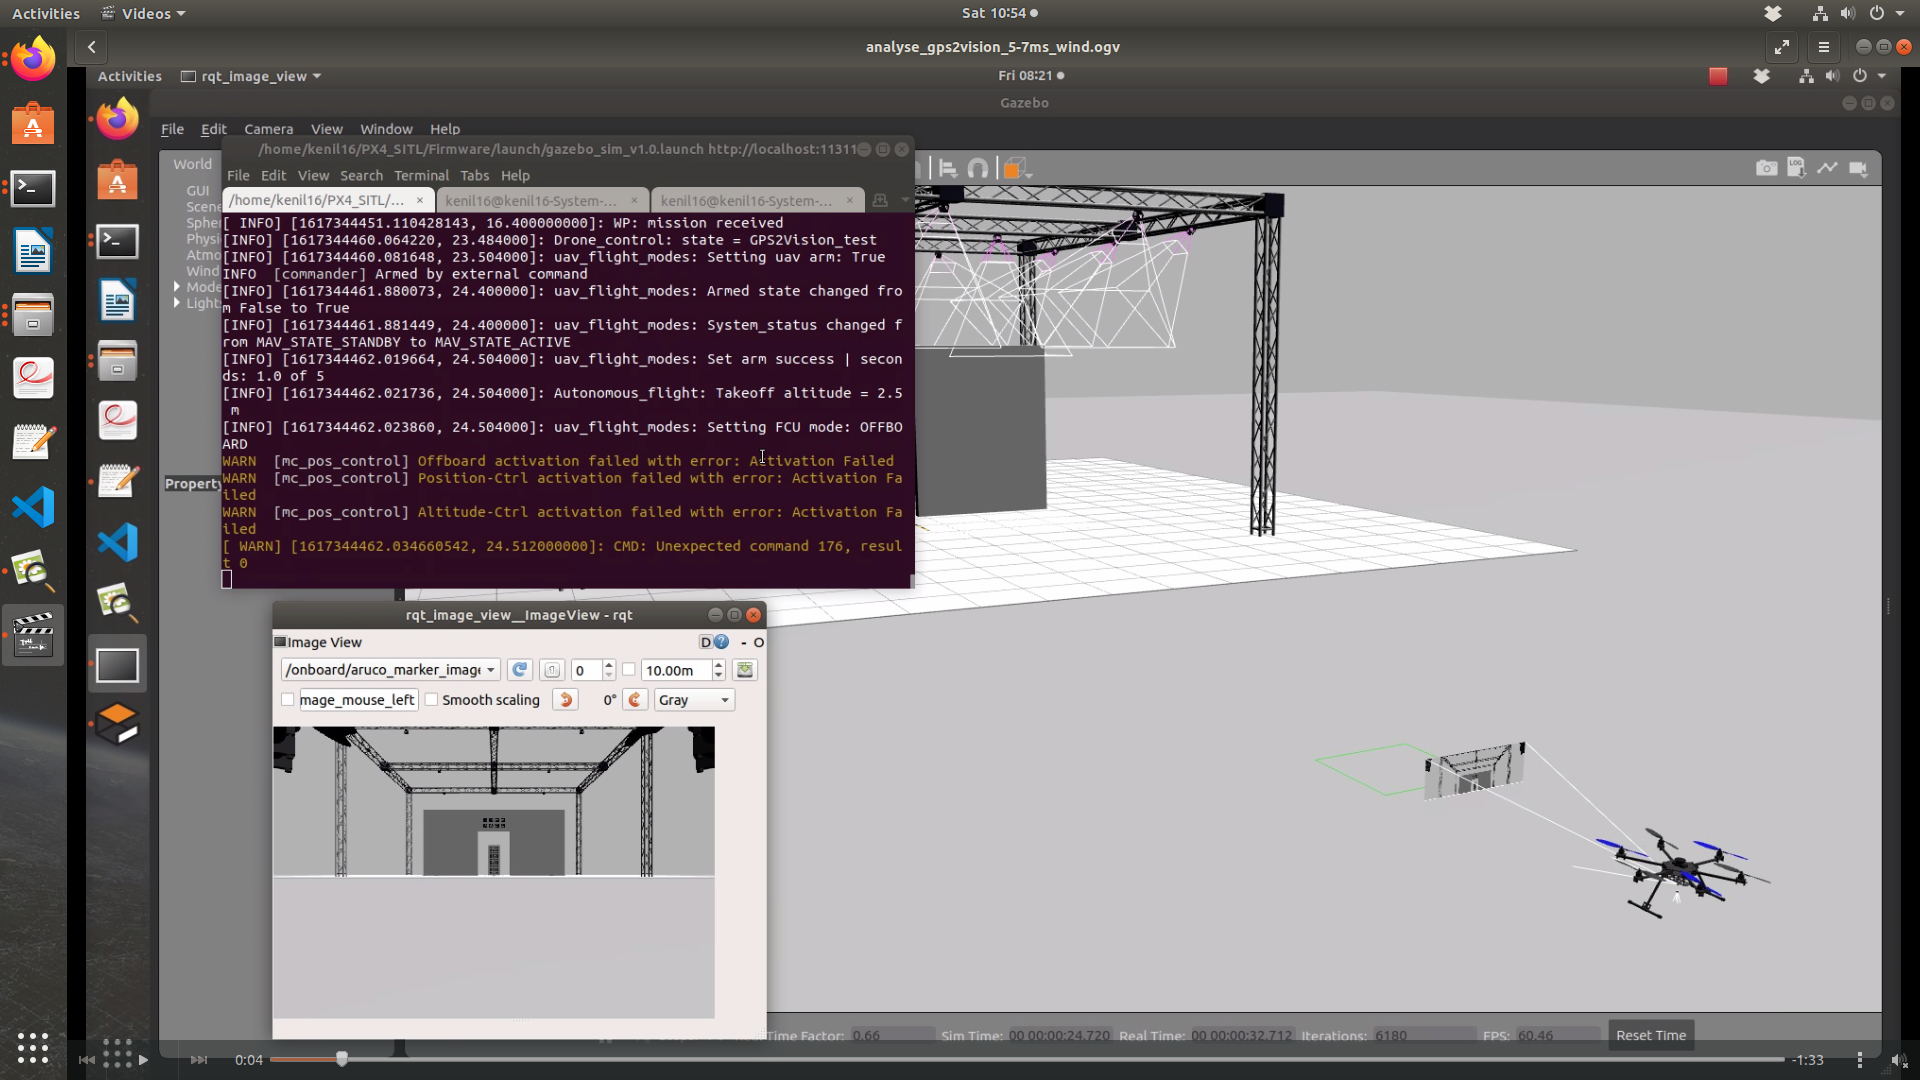
\includegraphics[width=\textwidth]{../Figures/GPS2Vision/drone_start_pose_gps.png}
        \caption{}
        \label{fig:gps2vision_gps}
    \end{subfigure}
     \hspace{0.2em}
    \begin{subfigure}[t]{.30\textwidth}
        \centering
        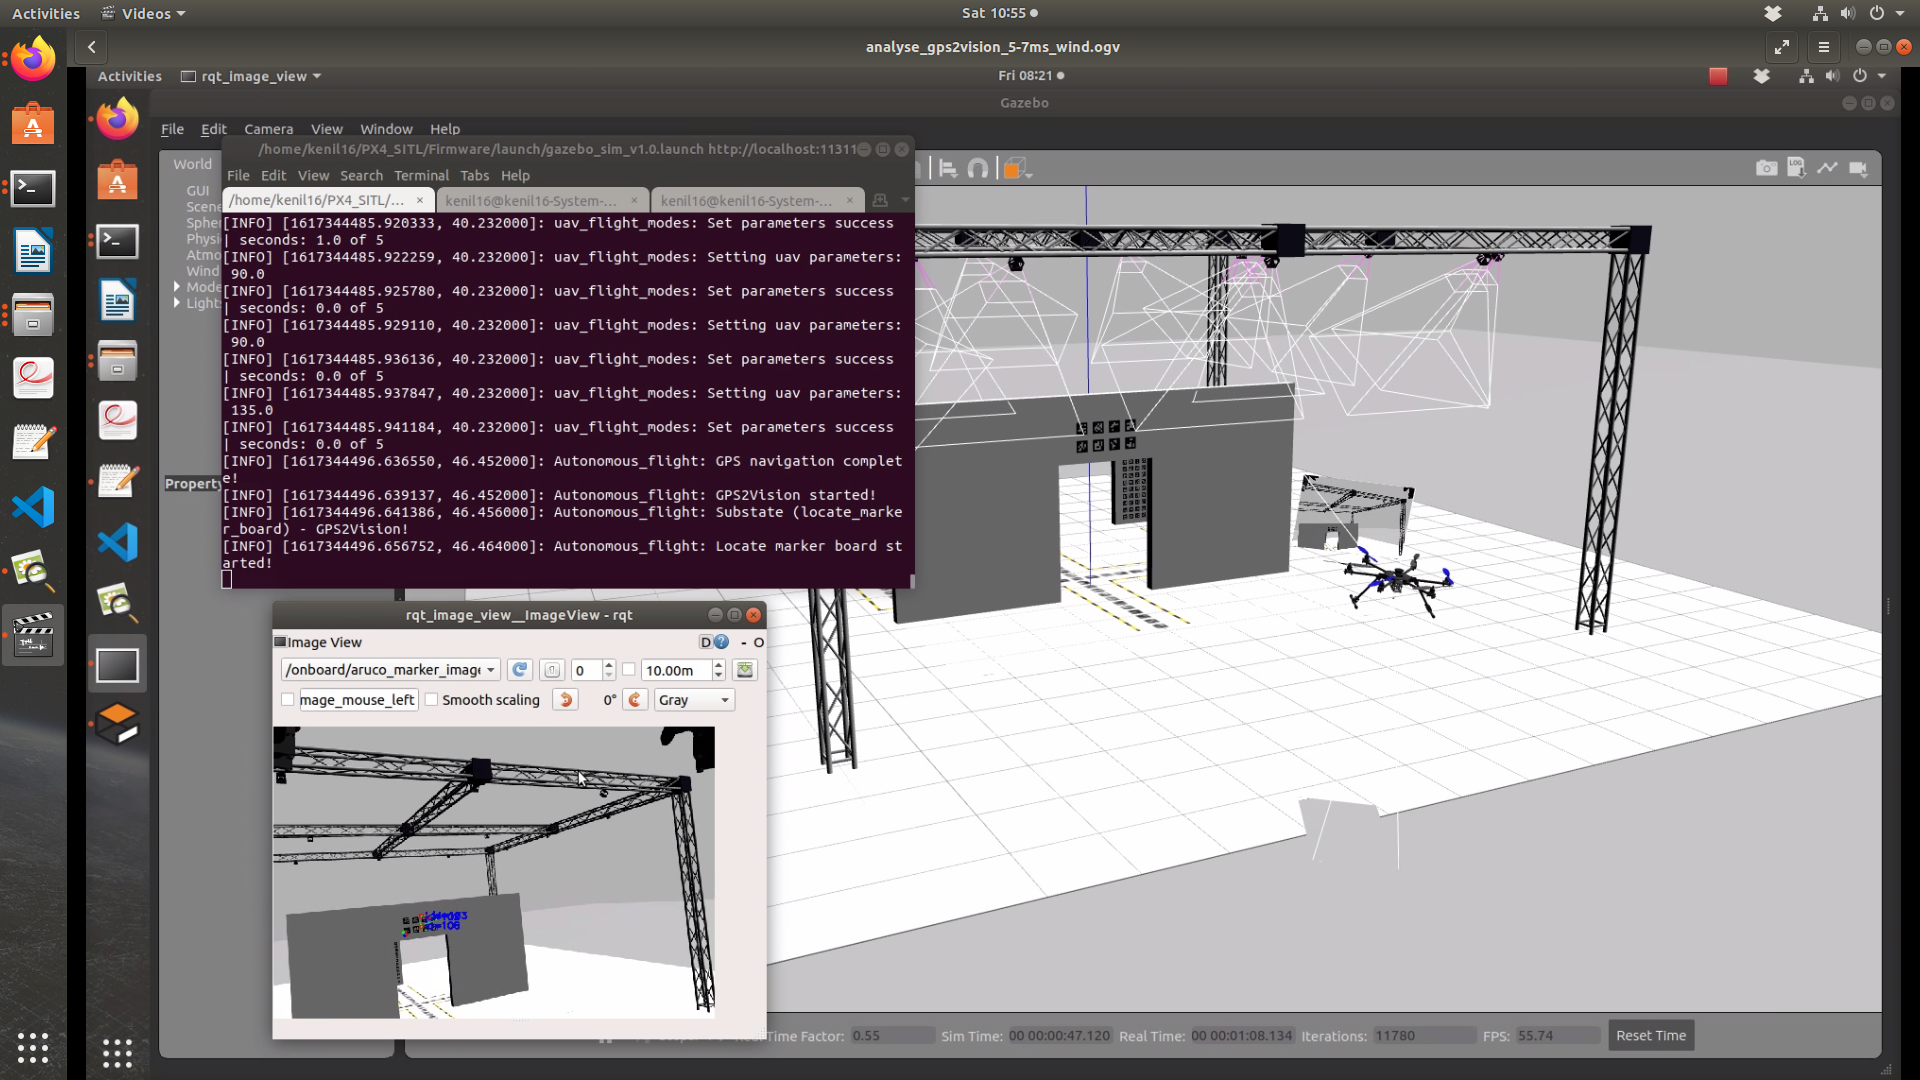
\includegraphics[width=\textwidth]{../Figures/GPS2Vision/drone_locate_board.png}
        \caption{}
        \label{fig:gps2vision_locate_board}
    \end{subfigure}
         \hspace{0.2em}
    \begin{subfigure}[t]{.30\textwidth}
        \centering
        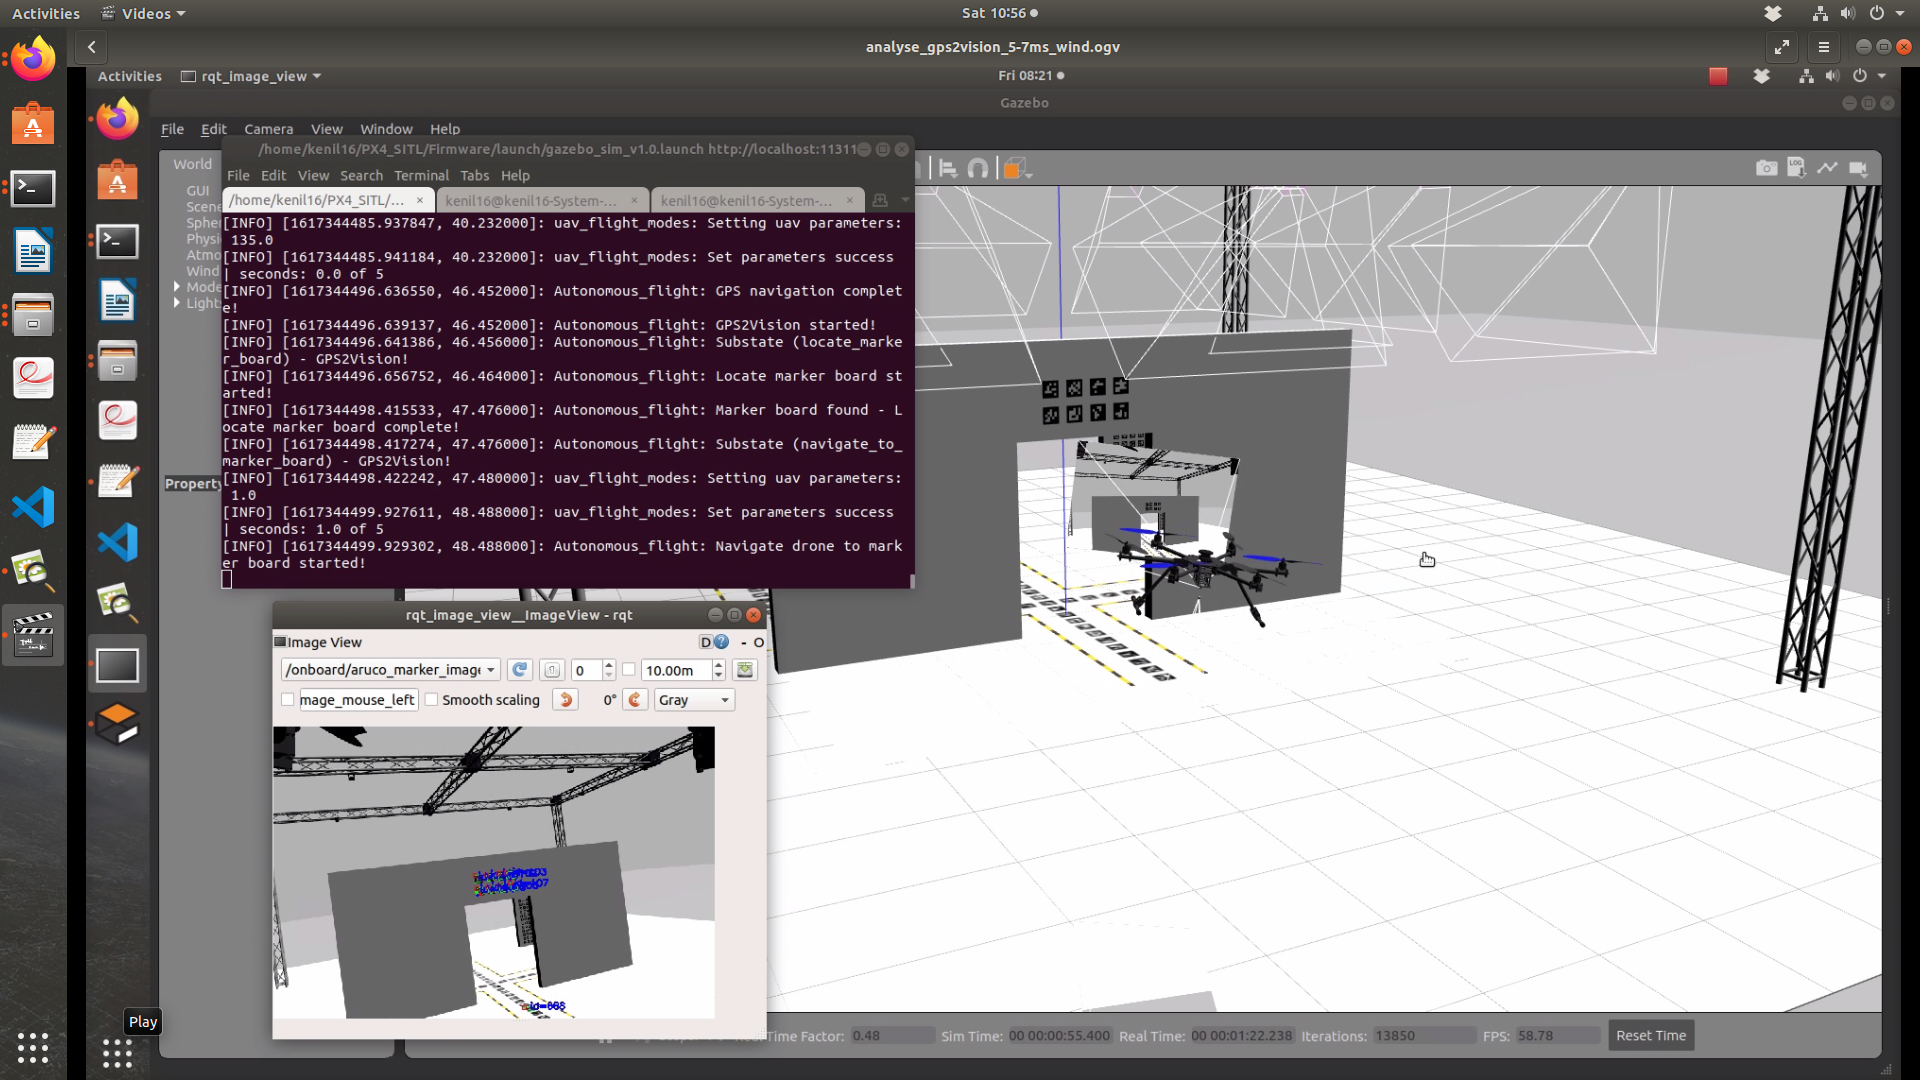
\includegraphics[width=\textwidth]{../Figures/GPS2Vision/drone_navigate_to_board.png}
        \caption{}
        \label{fig:gps2vision_navigate_to_board}
    \end{subfigure}
         \hspace{0.2em}
    \begin{subfigure}[t]{.30\textwidth}
        \centering
        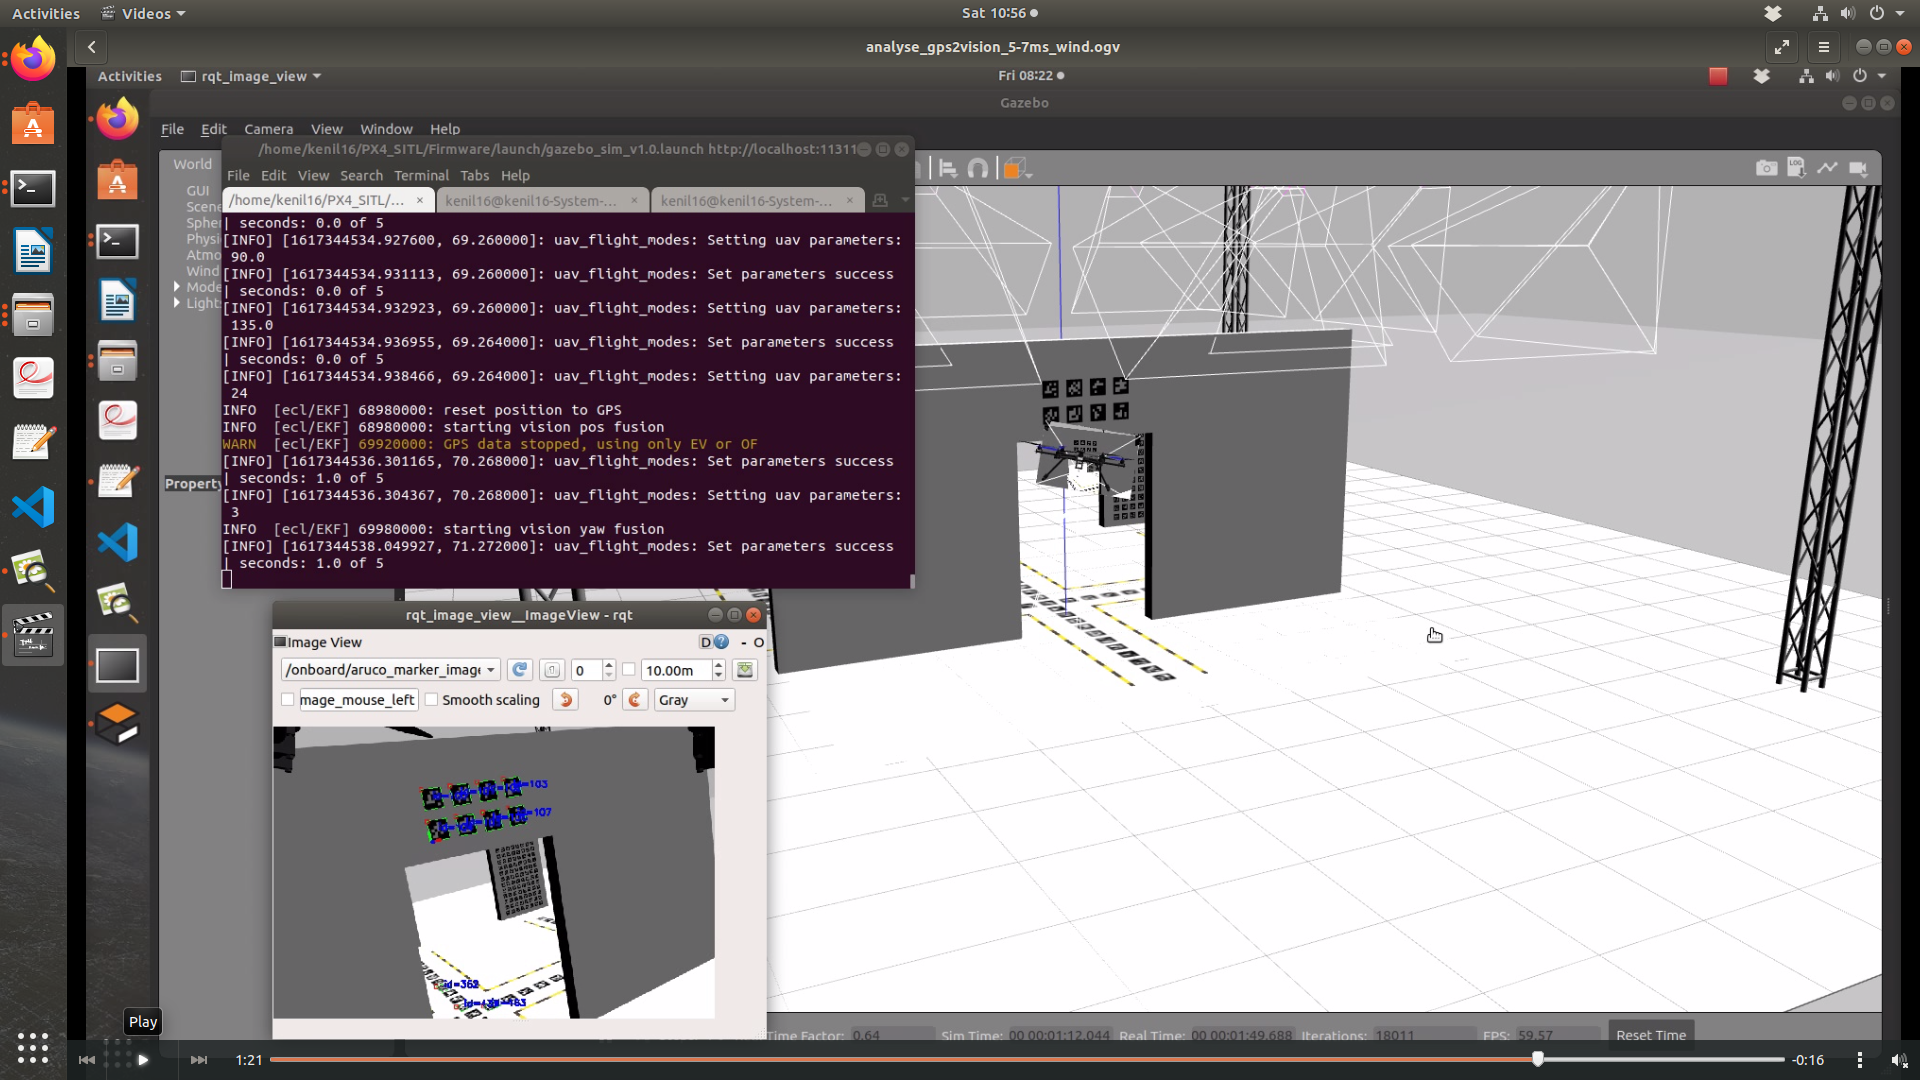
\includegraphics[width=\textwidth]{../Figures/GPS2Vision/drone_gps2vision_transition.png}
        \caption{}
        \label{fig:gps2vision_gps2vision_transition}
    \end{subfigure}
         \hspace{0.2em}
    \begin{subfigure}[t]{.30\textwidth}
        \centering
        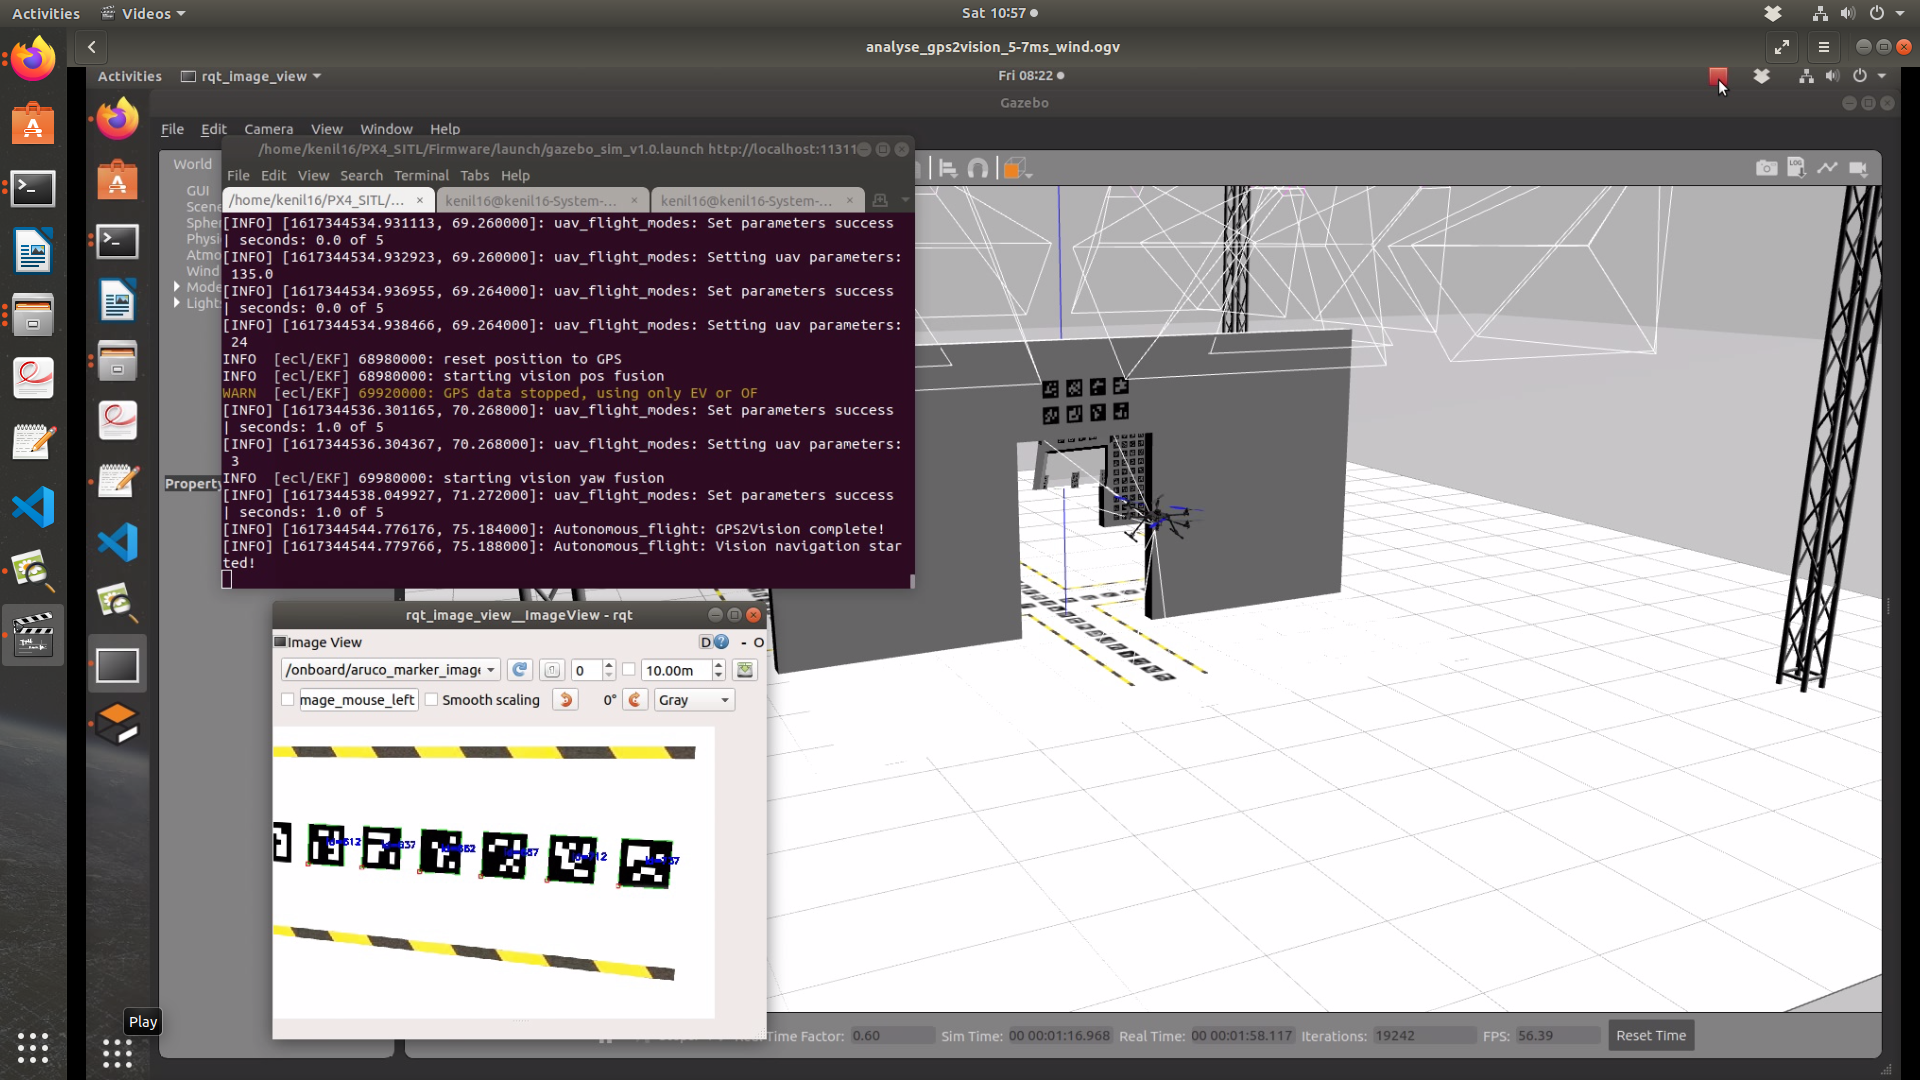
\includegraphics[width=\textwidth]{../Figures/GPS2Vision/drone_vision_navigation.png}
        \caption{}
        \label{fig:gps2vision_vision_navigation}
    \end{subfigure}
    \caption{}
    \label{fig:gps2vision_states}
\end{figure}

\begin{table}[H]
    \centering
    \addtolength{\leftskip} {-2cm}
    \addtolength{\rightskip}{-2cm}
        \caption{Statistics of the results from landing tests }
        \pgfplotstabletypeset[normal,
                columns/eg/.style={
                column name={Runs},
                dec sep align
        }
        ]{ %
       Wind & eg & Completed & Vel (GPS) & GPS & Locate board & Navigate to board & Vel (vision) & GPS2Vision\\
        \topmidheader{10}{\textbf{Test 1}}
          0 $\frac{m}{s}$ & 20 & 20 & $2\frac{m}{s}$ & $7.45s$ & $0.50s$ & $14.64s$ & $1\frac{m}{s}$ & $5.28s$\\
          \midheader{10}{\textbf{Test 2}}
               5-7 $\frac{m}{s}$ & 20 & 20 & $2 \frac{m}{s}$ & $6.66s$ & $1.76s$ & $16.05s$ & 1$\frac{m}{s}$ & $5.32s$\\
                  \midheader{10}{\textbf{Test 3}}
               7-10 $\frac{m}{s}$ & 20 & 17 & $2\frac{m}{s}$ & $7.04s$ & $3.71s$ & $16.24s$ & $1\frac{m}{s}$& $20.39s$\\
}
\end{table}


\begin{figure}[H]
    \centering
    \begin{subfigure}[t]{.45\textwidth}
        \centering
        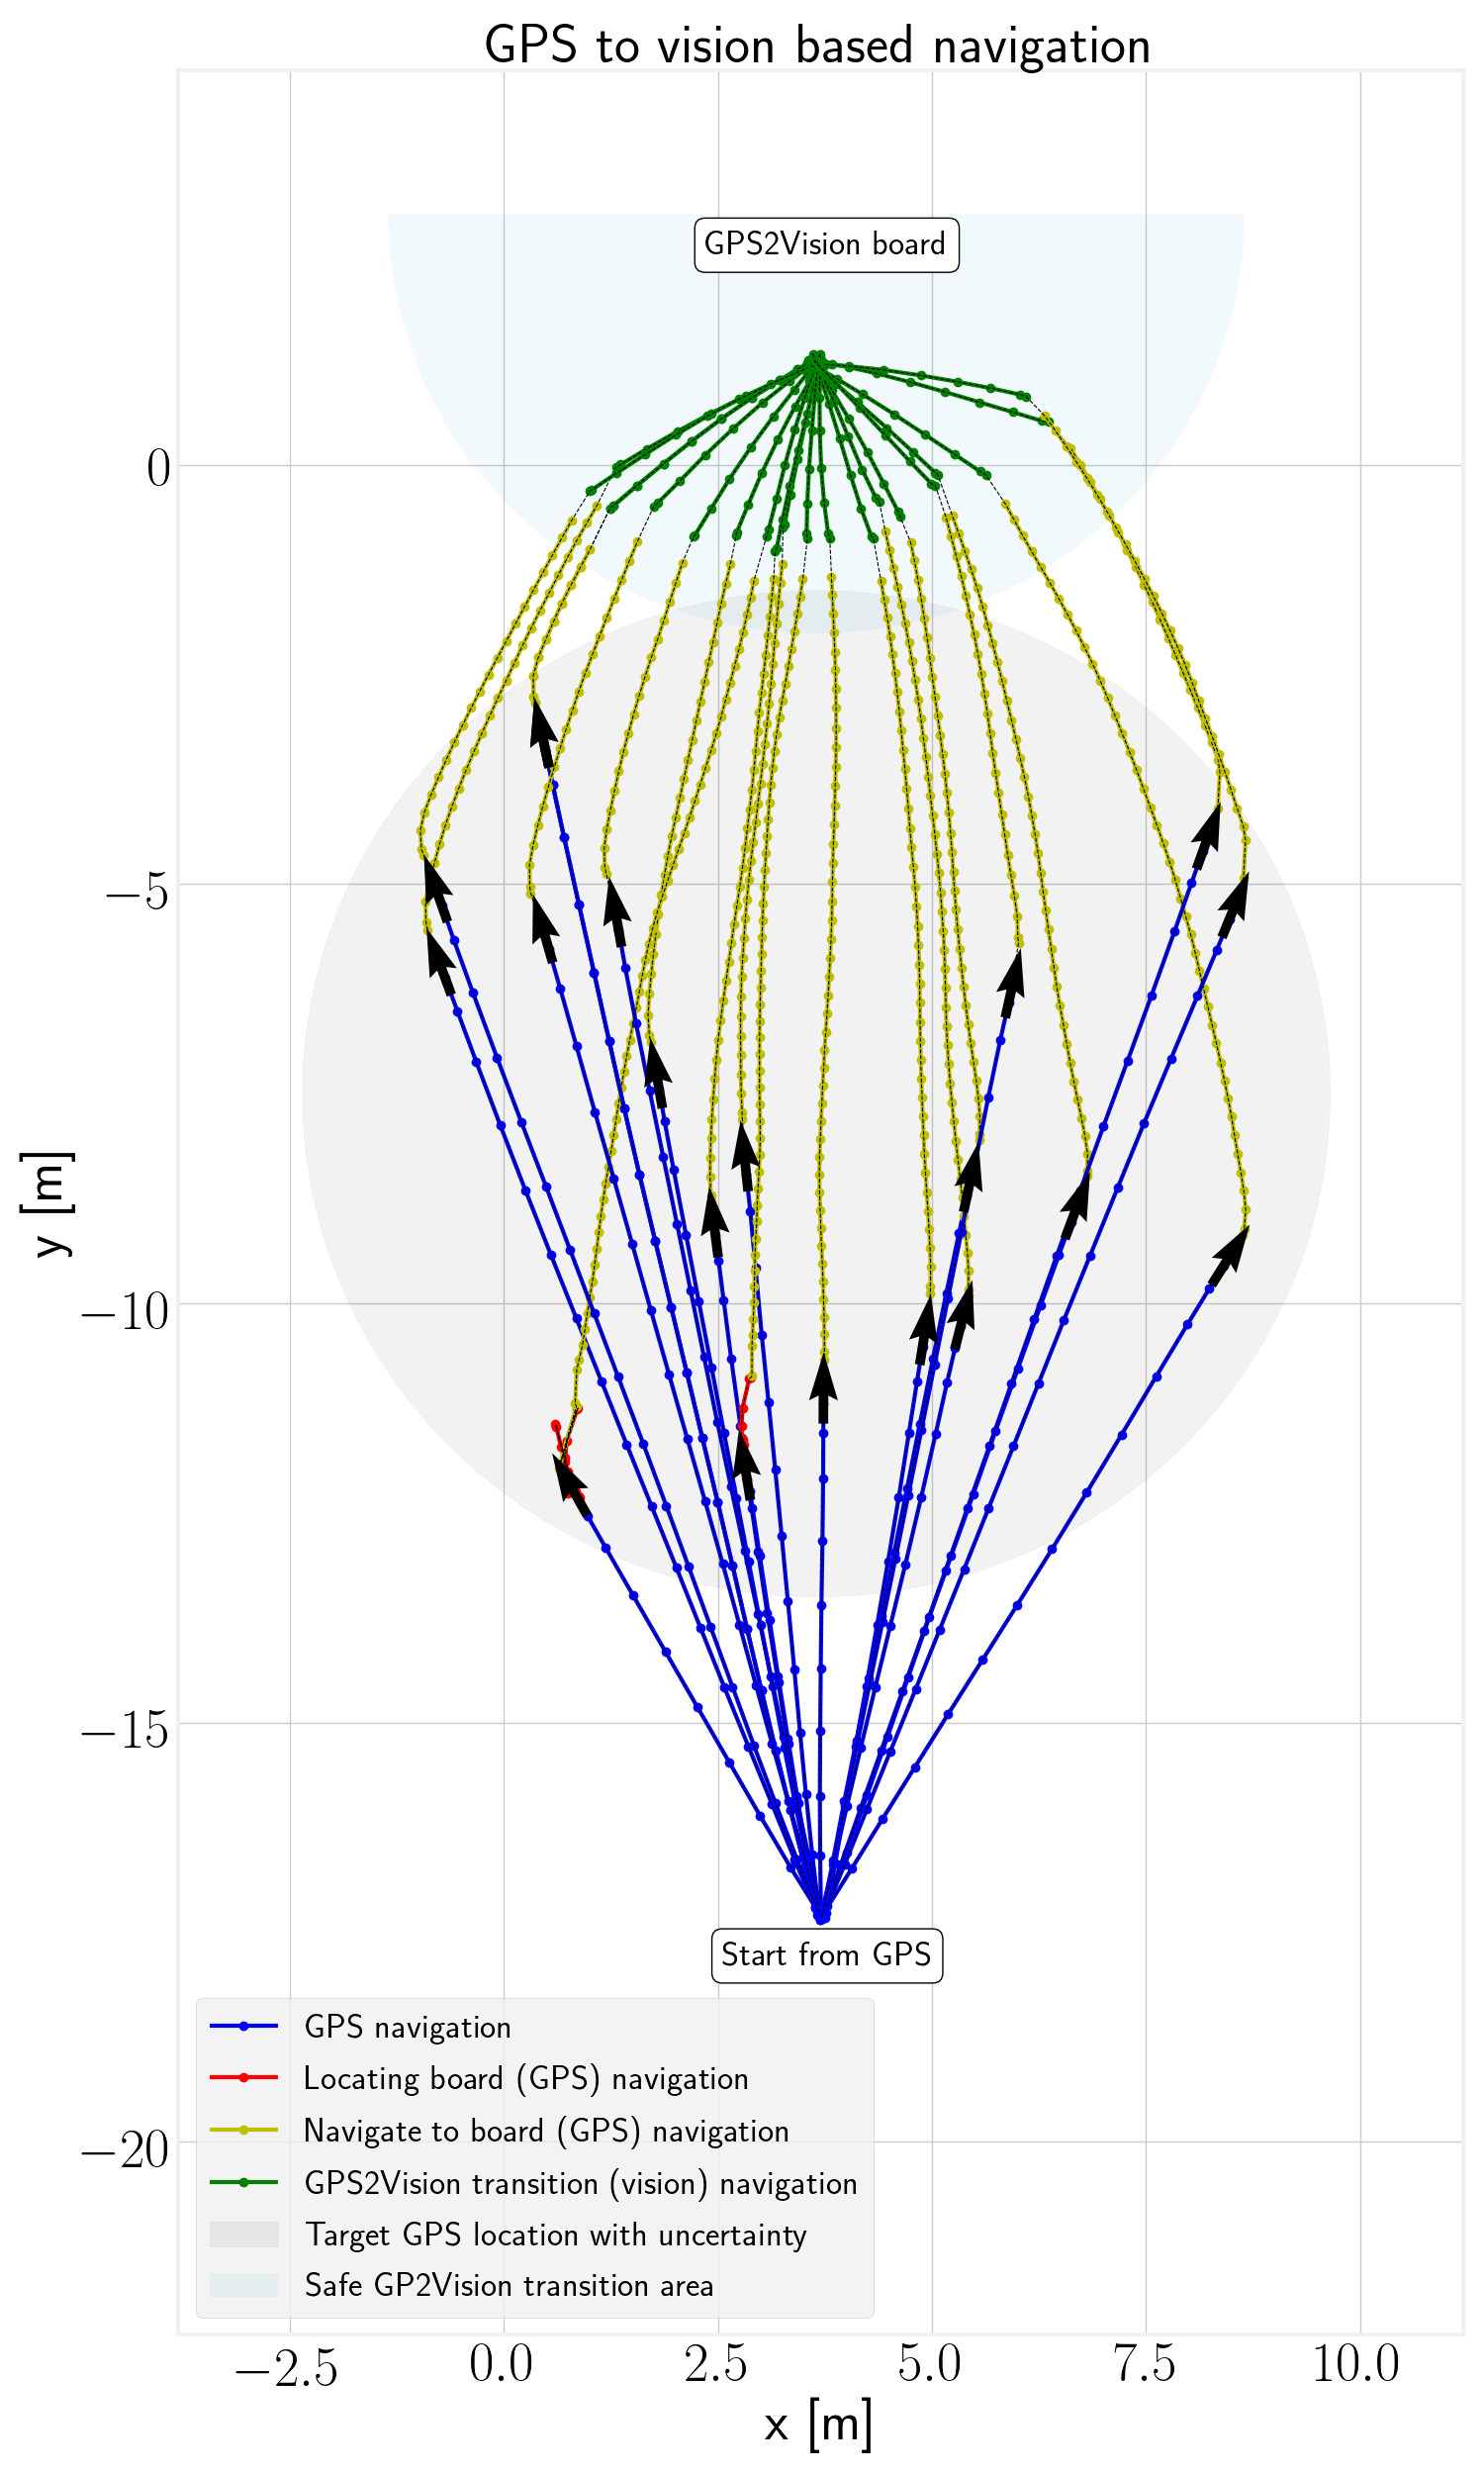
\includegraphics[width=\textwidth]{../Figures/GPS2Vision/test1_noWind_20_runs/gps2vision.png}
        \caption{}
        \label{fig:GPS2Vision_test1}
    \end{subfigure}
     \hspace{0.2em}
    \begin{subfigure}[t]{.45\textwidth}
        \centering
        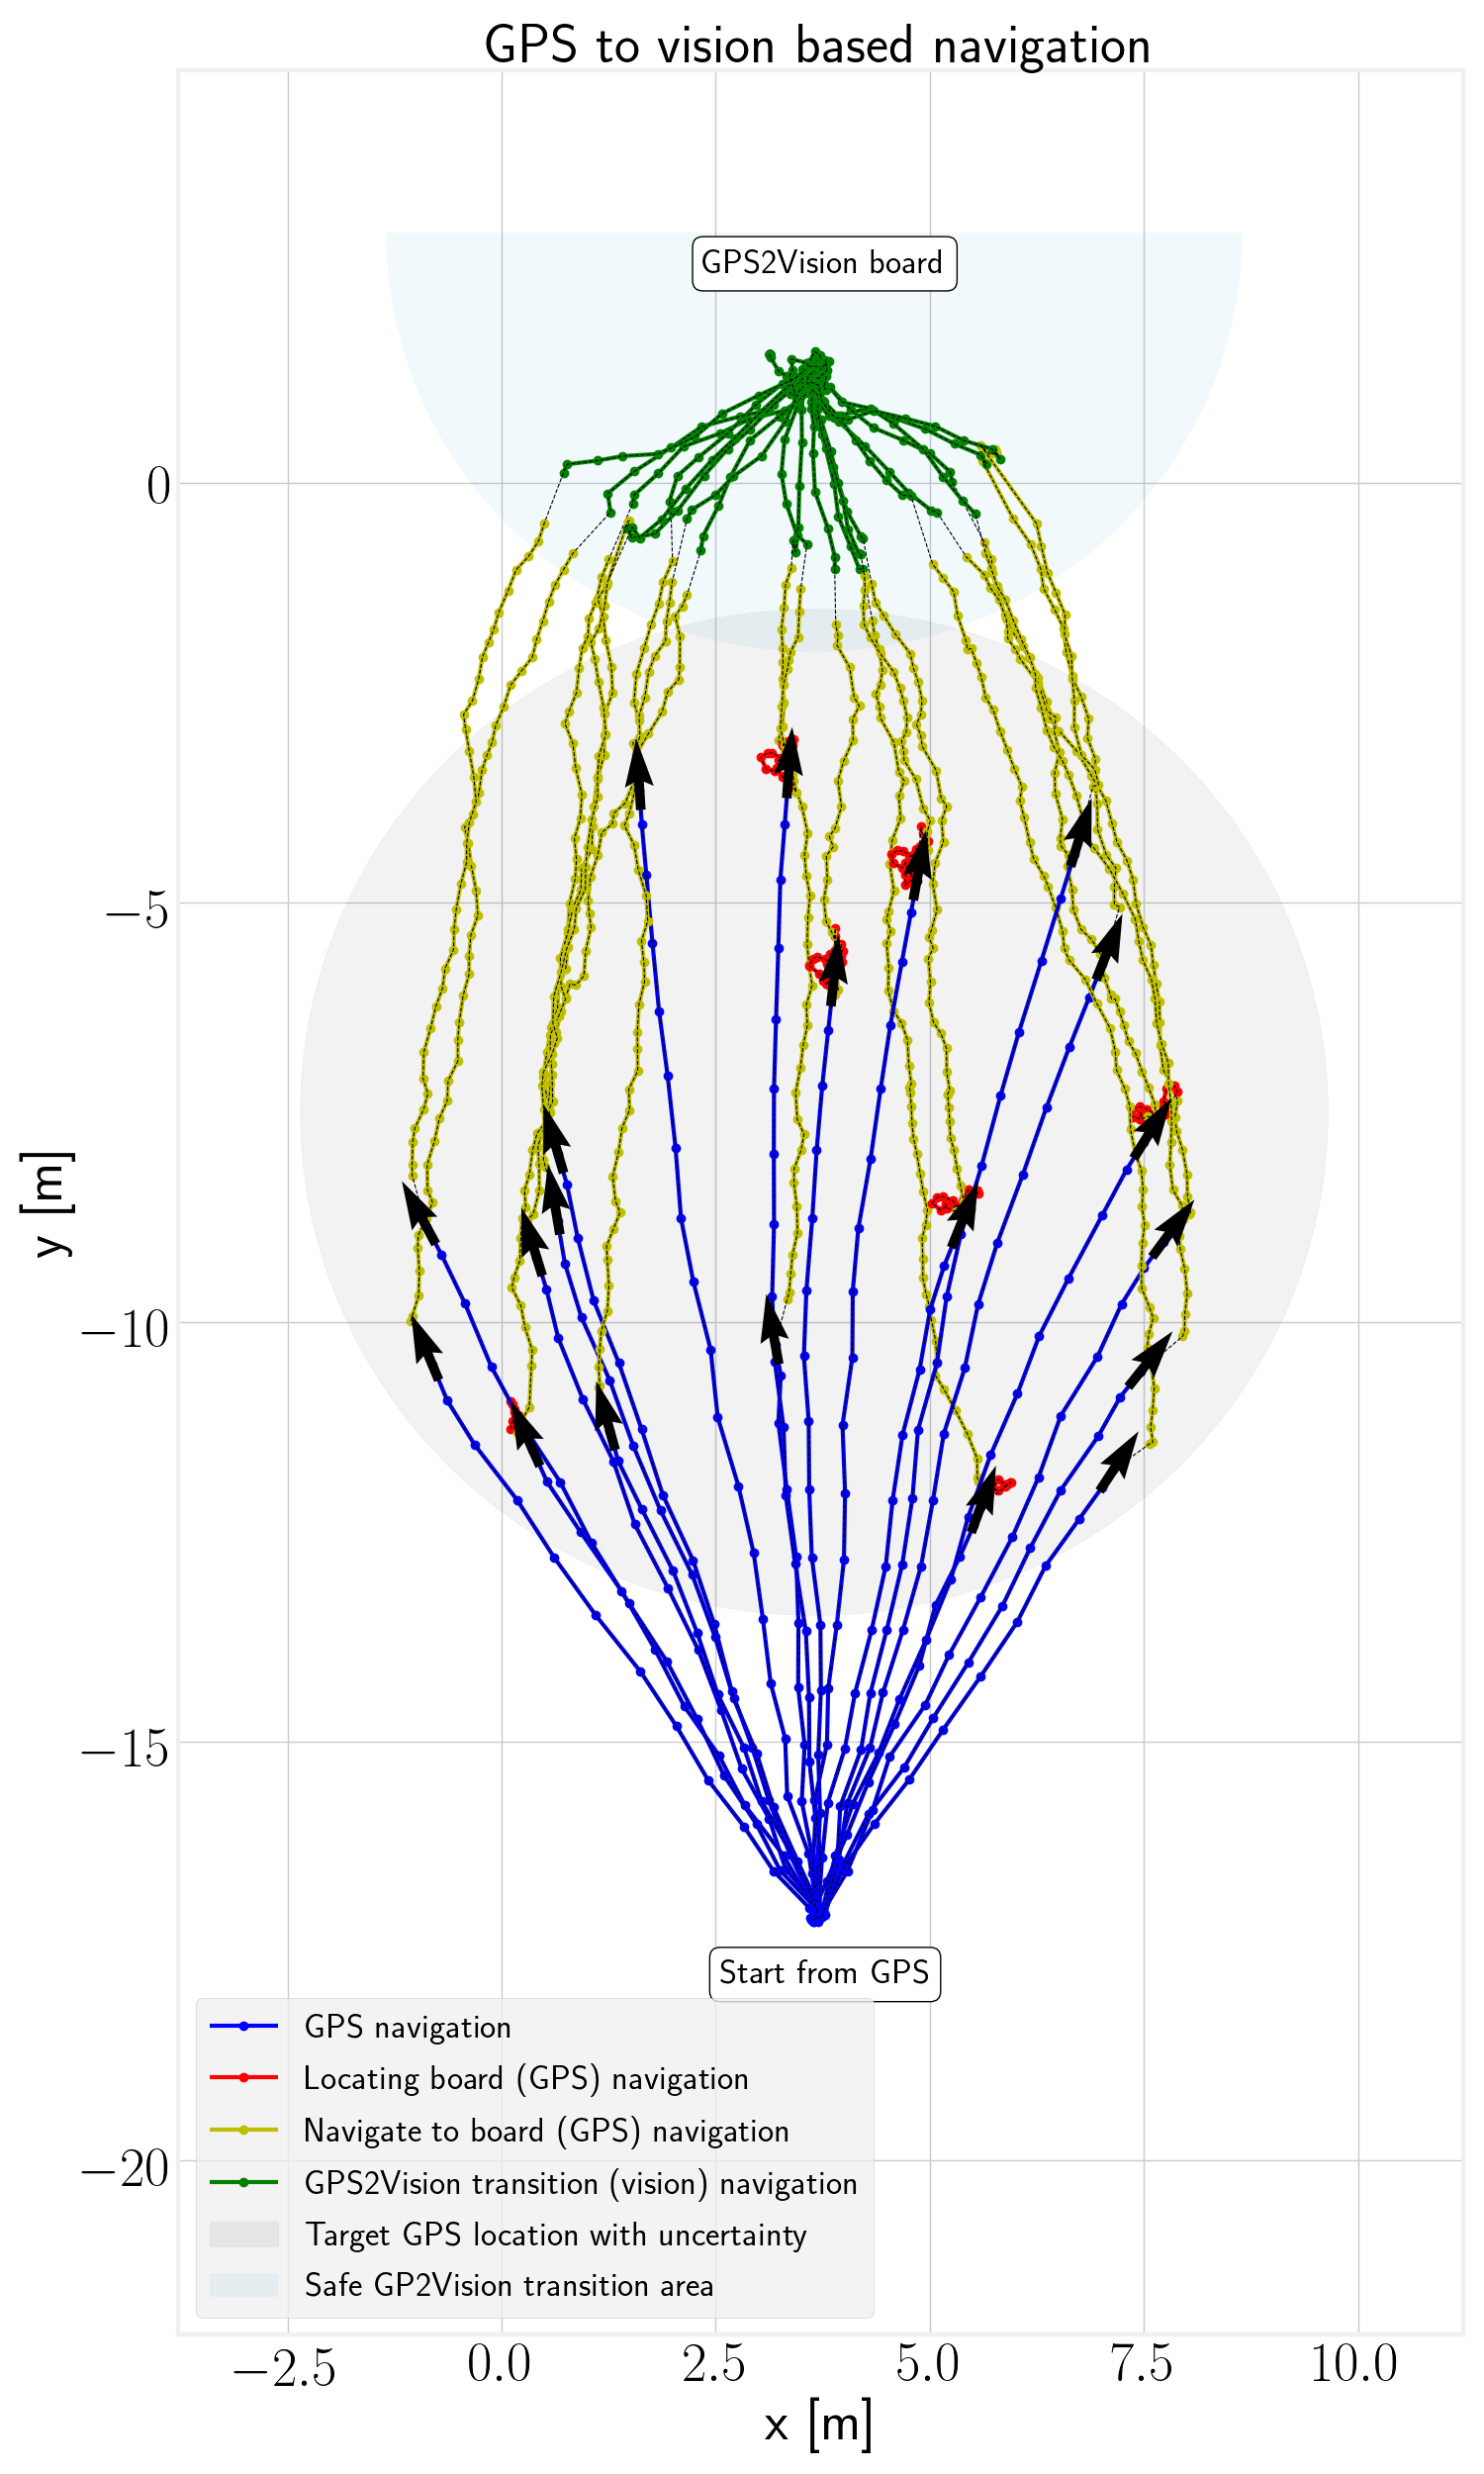
\includegraphics[width=\textwidth]{../Figures/GPS2Vision/test3_7-10ms_wind_20_runs/gps2vision.png}
        \caption{}
        \label{fig:GPS2Vision_test3}
    \end{subfigure}
    \caption{}
    \label{fig:GPS2Vision_test1_test3}
\end{figure}

\subsubsection{Vision based navigation}

\begin{figure}[H]
    \centering
    \begin{subfigure}[t]{.30\textwidth}
        \centering
        \includegraphics[width=\textwidth]{../Figures/vision_navigation/gps2vision.png}
        \caption{}
        \label{fig:vision_navigation_gps2vision}
    \end{subfigure}
     \hspace{0.2em}
    \begin{subfigure}[t]{.30\textwidth}
        \centering
        \includegraphics[width=\textwidth]{../Figures/vision_navigation/vision_navigation_one.png}
        \caption{}
        \label{fig:vision_navigation_vision_navigation_one}
    \end{subfigure}
     \hspace{0.2em}
    \begin{subfigure}[t]{.30\textwidth}
        \centering
        \includegraphics[width=\textwidth]{../Figures/vision_navigation/vision_navigation_two.png}
        \caption{}
        \label{fig:vision_navigation_vision_navigation_two}
    \end{subfigure}
    \caption{}
    \label{fig:vision_navigation}
\end{figure}

\begin{figure}[H]
    \centering
    \begin{subfigure}[t]{.20\textwidth}
        \centering
        \includegraphics[width=\textwidth]{../Figures/vision_navigation/grid_board_new_200_full.png}
        \caption{}
        \label{fig:vision_navigation_full_pattern_board}
    \end{subfigure}
     \hspace{0.2em}
    \begin{subfigure}[t]{.20\textwidth}
        \centering
        \includegraphics[width=\textwidth]{../Figures/vision_navigation/grid_board_new_200_big_onepattern.png}
        \caption{}
        \label{fig:vision_navigation_one_pattern_board}
    \end{subfigure}
     \hspace{0.2em}
    \begin{subfigure}[t]{.20\textwidth}
        \centering
        \includegraphics[width=\textwidth]{../Figures/vision_navigation/grid_board_new_200_big_onepattern_missing_markers1.png}
        \caption{}
        \label{fig:vision_navigation_one_pattern_board_missing_markers}
    \end{subfigure}
         \hspace{0.2em}
    \begin{subfigure}[t]{.20\textwidth}
        \centering
        \includegraphics[width=\textwidth]{../Figures/vision_navigation/grid_board_new_200_big_onepattern_missing_markers_wear.png}
        \caption{}
        \label{fig:vision_navigation_one_pattern_board_missing_markers_wear}
    \end{subfigure}
    \caption{}
    \label{fig:vision_navigation_boards}
\end{figure}

\begin{table}[H]
    \centering
    \addtolength{\leftskip} {-2cm}
    \addtolength{\rightskip}{-2cm}
        \caption{Statistics of the results from landing tests }
        \pgfplotstabletypeset[normal,
                columns/eg/.style={
                column name={Runs},
                dec sep align
        }
        ]{ %
        Estimation error & eg & Waypoint error & Vel (Horizontal) & Mean position & STD position & Mean angle & STD angle\\
        \topmidheader{8}{\textbf{Test 1}}
        ArUco pose & 20 & $0.1 m$ & $1\frac{m}{s}$ & $2.44cm$ & $2.51cm$ & $1.59 ^{\circ}$ & $9.68^{\circ}$\\
        \midheader{8}{\textbf{Test 2}}
        ArUco pose & 20 & $0.1 m$ & $1\frac{m}{s}$ &$2.44cm$ & $2.29cm$ & $1.30 ^{\circ}$ & $7.44^{\circ}$\\
        \midheader{8}{\textbf{Test 3}}
        ArUco pose & 20 & $0.1 m$ & $1\frac{m}{s}$ & $3.19cm$ & $3.28cm$ & $1.99 ^{\circ}$ & $10.88^{\circ}$\\
        \midheader{8}{\textbf{Test 4}}
        ArUco pose & 20 & $0.1 m$ & $1\frac{m}{s}$ & $4.21cm$ & $3.96cm$ & $3.09 ^{\circ}$ & $11.99^{\circ}$\\
        \midheader{8}{\textbf{Test 5}}
        ArUco pose & 20 & $0.1 m$ & $5\frac{m}{s}$ & $5.66cm$ & $5.79cm$ & $6.89 ^{\circ}$ & $22.29^{\circ}$\\}
\end{table}

\begin{figure}[H]
    \centering
    \begin{subfigure}[t]{.30\textwidth}
        \centering
        \includegraphics[width=\textwidth]{../Figures/vision_navigation/test1_full_pattern_board/2d_path.png}
        \caption{}
        \label{fig:vision_navigation_2d_path_full_board}
    \end{subfigure}
     \hspace{0.2em}
    \begin{subfigure}[t]{.30\textwidth}
        \centering
        \includegraphics[width=\textwidth]{../Figures/vision_navigation/test4_one_pattern_missing_markers_wear_board/2d_path.png}
        \caption{}
        \label{fig:vision_navigation_2d_path_missing_markers_wear_vel_1.0}
    \end{subfigure}
     \hspace{0.2em}
    \begin{subfigure}[t]{.30\textwidth}
        \centering
        \includegraphics[width=\textwidth]{../Figures/vision_navigation/test5_one_pattern_missing_markers_wear_board/2d_path.png}
        \caption{}
        \label{fig:vision_navigation_2d_path_missing_markers_wear_vel_5.0}
    \end{subfigure}
    \caption{}
    \label{fig:vision_navigation_2d_path}
\end{figure}

\begin{figure}[H]
    \centering
    \begin{subfigure}[t]{.30\textwidth}
        \centering
        \includegraphics[width=\textwidth]{../Figures/vision_navigation/test1_full_pattern_board/error_x/pose_error_x_test1.png}
        \caption{}
        \label{fig:vision_navigation_error_x}
    \end{subfigure}
     \hspace{0.2em}
    \begin{subfigure}[t]{.30\textwidth}
        \centering
        \includegraphics[width=\textwidth]{../Figures/vision_navigation/test1_full_pattern_board/error_y/pose_error_y_test1.png}
        \caption{}
        \label{fig:vision_navigation_error_y}
    \end{subfigure}
     \hspace{0.2em}
    \begin{subfigure}[t]{.30\textwidth}
        \centering
        \includegraphics[width=\textwidth]{../Figures/vision_navigation/test1_full_pattern_board/error_z/pose_error_z_test1.png}
        \caption{}
        \label{fig:vision_navigation_error_z}
    \end{subfigure}
    \caption{}
    \label{fig:vision_navigation_error_pos}
\end{figure}

\begin{figure}[H]
    \centering
    \begin{subfigure}[t]{.30\textwidth}
        \centering
        \includegraphics[width=\textwidth]{../Figures/vision_navigation/test1_full_pattern_board/error_roll/pose_error_roll_test1.png}
        \caption{}
        \label{fig:vision_navigation_error_roll}
    \end{subfigure}
     \hspace{0.2em}
    \begin{subfigure}[t]{.30\textwidth}
        \centering
        \includegraphics[width=\textwidth]{../Figures/vision_navigation/test1_full_pattern_board/error_pitch/pose_error_pitch_test1.png}
        \caption{}
        \label{fig:vision_navigation_error_pitch}
    \end{subfigure}
     \hspace{0.2em}
    \begin{subfigure}[t]{.30\textwidth}
        \centering
        \includegraphics[width=\textwidth]{../Figures/vision_navigation/test1_full_pattern_board/error_yaw/pose_error_yaw_test1.png}
        \caption{}
        \label{fig:vision_navigation_error_yaw}
    \end{subfigure}
    \caption{}
    \label{fig:vision_navigation_error_angle}
\end{figure}

\subsubsection{Vision based landing}

\begin{figure}[H]
    \centering
    \begin{subfigure}[t]{.30\textwidth}
        \centering
        \includegraphics[width=\textwidth]{../Figures/landing_test/landing_station_one.png}
        \caption{}
        \label{fig:vision_based_landing_landing_station_one}
    \end{subfigure}
     \hspace{0.2em}
    \begin{subfigure}[t]{.30\textwidth}
        \centering
        \includegraphics[width=\textwidth]{../Figures/landing_test/landing_station_two.png}
        \caption{}
        \label{fig:vision_based_landing_landing_station_two}
    \end{subfigure}
     \hspace{0.2em}
    \begin{subfigure}[t]{.30\textwidth}
        \centering
        \includegraphics[width=\textwidth]{../Figures/landing_test/landing_station_three.png}
        \caption{}
        \label{fig:vision_based_landing_landing_station_three}
    \end{subfigure}
    \caption{}
    \label{fig:vision_based_landing_landing_stations}
\end{figure}

\begin{table}[H]
    \centering
    \addtolength{\leftskip} {-2cm}
    \addtolength{\rightskip}{-2cm}
        \caption{Statistics of the results from landing tests }
        \pgfplotstabletypeset[normal,
                columns/eg/.style={
                column name={Runs},
                dec sep align
        }
        ]{ %
        Station & eg & Waypoint error & Velocity & Min & Max & Mean & STD & Stabilize time & Landing time\\
        \topmidheader{11}{\textbf{Test 1}}
        One         & 35      & $0.1 m$ & $0.1 \frac{m}{s}$ & $1.60cm$ & $12.46cm$ & $5.81cm$ & $3.02cm$ & $3.60s$ &$11.51s$\\
        two         & 30     & $0.1 m$ & $0.1 \frac{m}{s}$ & $0.70cm$ & $11.83 cm$& $5.79cm$ & $2.54cm$& $0.70s$ &$11.76s$\\     
        Three       & 35     & $0.1 m$ & $0.1 \frac{m}{s}$ & $0.62cm$ & $10.75cm$ & $5.86cm$ & $2.50cm$& $3.22s$ &$11.82s$\\    
        \midheader{11}{\textbf{Test 2}}
        One         & 33      & $0.1 m$ & $0.5 \frac{m}{s}$ & $2.20cm$ & $15.04cm$ & $8.00cm$ & $2.67cm$ & $2.63s$ &$3.00s$\\
        two         & 29     & $0.1 m$ & $0.5 \frac{m}{s}$ & $3.18cm$ & $11.60 cm$& $7.62cm$ & $2.19cm$& $0.20s$ &$3.00s$\\     
        Three       & 38     & $0.1 m$ & $0.5 \frac{m}{s}$ & $1.11cm$ & $14.63cm$ & $7.87cm$ & $3.25cm$& $2.18s$ &$3.02s$\\    
        \midheader{11}{\textbf{Test 3}}
        One         & 32      & $0.1 m$ & $0.9 \frac{m}{s}$ & $4.63cm$ & $14.01cm$ & $9.25cm$ & $2.27cm$ & $1.68s$ &$2.15s$\\
        two         & 36    & $0.1 m$ & $0.9 \frac{m}{s}$ & $4.79cm$ & $14.00 cm$& $9.54cm$ & $1.92cm$& $0.19s$ &$2.13s$\\     
        Three       & 32     & $0.1 m$ & $0.9 \frac{m}{s}$ & $3.35cm$ & $18.45cm$ & $9.45cm$ & $2.88cm$& $2.09s$ &$2.18s$\\}
\end{table}

\begin{table}[H]
    \centering
    \addtolength{\leftskip} {-2cm}
    \addtolength{\rightskip}{-2cm}
        \caption{Statistics of the results from landing tests }
        \pgfplotstabletypeset[normal,
                columns/eg/.style={
                column name={Runs},
                dec sep align
        }
        ]{ %
        Station & eg & Waypoint error & Velocity & Min & Max & Mean & STD & Stabilize time & Landing time\\
        \topmidheader{11}{\textbf{Test 4}}
One         & 33      & $0.05 m$ & $0.1 \frac{m}{s}$ & $0.08cm$ & $9.46cm$ & $4.81cm$ & $2.15cm$ & $9.93s$ &$11.45s$\\
        two         & 33    & $0.05 m$ & $0.1 \frac{m}{s}$ & $0.97cm$ & $11.18 cm$& $4.74cm$ & $2.56cm$& $6.96s$ &$11.69s$\\     
        Three       & 34     & $0.05 m$ & $0.1 \frac{m}{s}$ & $0.19cm$ & $11.84cm$ & $4.54cm$ & $2.41cm$& $9.11s$ &$11.58s$\\        		\midheader{11}{\textbf{Test 5}}
        One         & 32     & $0.05 m$ & $0.5 \frac{m}{s}$ & $1.63cm$ & $9.84cm$ & $5.25cm$ & $2.36cm$ & $8.43s$ &$3.00s$\\
        two         & 32    & $0.05 m$ & $0.5 \frac{m}{s}$ & $1.31cm$ & $13.07 cm$& $5.98cm$ & $2.90cm$& $6.34s$ &$3.00s$\\     
        Three       & 36     & $0.05 m$ & $0.5 \frac{m}{s}$ & $0.45cm$ & $12.22cm$ & $4.98cm$ & $2.88cm$& $9.33s$ &$3.00s$\\				\midheader{11}{\textbf{Test 6}}
        One         & 32     & $0.05 m$ & $0.9 \frac{m}{s}$ & $0.20cm$ & $11.89cm$ & $4.96cm$ & $2.77cm$ & $9.18s$ &$2.28s$\\
        two         & 35    & $0.05 m$ & $0.9 \frac{m}{s}$ & $0.65cm$ & $14.13 cm$& $5.90cm$ & $3.32cm$& $5.91s$ &$2.34s$\\     
        Three       & 33     & $0.05 m$ & $0.9 \frac{m}{s}$ & $1.06cm$ & $13.54cm$ & $5.35cm$ & $2.70cm$& $8.54s$ &$2.36s$\\}
\end{table}


\begin{figure}[H]
    \centering
    \begin{subfigure}[t]{.30\textwidth}
        \centering
        \includegraphics[width=\textwidth]{../Figures/landing_test/test3_speed_0.9_error_0.1/landing_for_station_one.png}
        \caption{}
        \label{fig:vision_based_landing_landing_station_one_test3}
    \end{subfigure}
     \hspace{0.2em}
    \begin{subfigure}[t]{.30\textwidth}
        \centering
        \includegraphics[width=\textwidth]{../Figures/landing_test/test3_speed_0.9_error_0.1/landing_for_station_two.png}
        \caption{}
        \label{fig:vision_based_landing_landing_station_two_test3}
    \end{subfigure}
     \hspace{0.2em}
    \begin{subfigure}[t]{.30\textwidth}
        \centering
        \includegraphics[width=\textwidth]{../Figures/landing_test/test3_speed_0.9_error_0.1/landing_for_station_three.png}
        \caption{}
        \label{fig:vision_based_landing_landing_station_three_test3}
    \end{subfigure}
    \caption{}
    \label{fig:vision_based_landing_test3}
\end{figure}

\begin{figure}[H]
    \centering
    \begin{subfigure}[t]{.30\textwidth}
        \centering
        \includegraphics[width=\textwidth]{../Figures/landing_test/test4_speed_0.1_error_0.05/landing_for_station_one.png}
        \caption{}
        \label{fig:vision_based_landing_landing_station_one_test4}
    \end{subfigure}
     \hspace{0.2em}
    \begin{subfigure}[t]{.30\textwidth}
        \centering
        \includegraphics[width=\textwidth]{../Figures/landing_test/test4_speed_0.1_error_0.05/landing_for_station_two.png}
        \caption{}
        \label{fig:vision_based_landing_landing_station_two_test4}
    \end{subfigure}
     \hspace{0.2em}
    \begin{subfigure}[t]{.30\textwidth}
        \centering
        \includegraphics[width=\textwidth]{../Figures/landing_test/test4_speed_0.1_error_0.05/landing_for_station_three.png}
        \caption{}
        \label{fig:vision_based_landing_landing_station_three_test4}
    \end{subfigure}
    \caption{}
    \label{fig:vision_based_landing_test4}
\end{figure}

\end{document}